\documentclass[12pt,a4paper,oneside,openright]{book}

%***********Main packages****************
%======================================================================
% 	   PACKAGES USEFUL TO FORMAT AND COMPILE EVERY LaTeX DOCUMENT
%======================================================================

%*********Document formatting****************
\usepackage[T1]{fontenc}
\usepackage[utf8]{inputenc}
\usepackage[a4paper,top=3cm,bottom=3cm,,left=3.5cm,right=3.5cm]{geometry}
\usepackage[english]{babel}
\usepackage{fmtcount}

%************Line spacing********************
\usepackage{setspace}

%************Footnote setup******************
\usepackage[bottom]{footmisc}
\setlength\footnotemargin{10pt}

%**************Caption setup*****************
\usepackage{caption}[2004/07/16]
\captionsetup{
	tableposition=top,
	figureposition=bottom,
	labelfont={sf,bf},
	singlelinecheck=false,
	margin=1cm
	}

%***********Tables utilities*****************
\usepackage{multicol}
\usepackage{multirow}
\usepackage{makecell}
\renewcommand{\cellalign}{l}

%***********Figures utilities****************
\usepackage{graphicx}
\usepackage{float}
\usepackage{subfig}

%***************Math setup*******************
\usepackage{amsmath}
\usepackage{amsfonts}
\usepackage{amssymb}
\usepackage{mathtools}
\usepackage{siunitx}

%*************Hyperlink setup****************
\usepackage[pdftex]{hyperref}
\hypersetup{
    colorlinks=true,
    linkcolor=blue,
    filecolor=blue,
    citecolor=blue,      
    linktocpage=true
}

%************Bibliography cite***************
\usepackage{cite}

%****************Appendices******************
\usepackage[titletoc]{appendix}

%***********Font packages****************
%==========================================================
%		EBGARAMOND FONT SETUP WITH MATH EXTENSION
%==========================================================

%*****************Definitions**********************
\usepackage{ebgaramond}
\usepackage{ebgaramond-maths}

%***********Add missing font symbols***************
\usepackage[cmintegrals,cmbraces]{newtxmath}
\makeatletter
	\DeclareSymbolFont{ntxletters}{OML}{ntxmi}{m}{it}
	\SetSymbolFont{ntxletters}{bold}{OML}{ntxmi}{b}{it}
	\re@DeclareMathSymbol{\partial}{\mathord}{ntxletters}{"40}
	\re@DeclareMathAccent{\vec}{\mathord}{ntxletters}{"7E}
\makeatother

%*****To enlarge epsilon symbol*******
%	\mathlarger{\mathlarger{\epsilon}}
\usepackage{relsize}

%******Feynman diagrams utilities********
\usepackage[compat=1.1.0]{tikz-feynman}

%***************Styles*******************
\linespread{1.2}
\pagestyle{plain}
%\usepackage{lineno}
%\linenumbers

%********Include figures' paths**********
\graphicspath{{immagini/}{immagini/capitolo_1/}{immagini/capitolo_2/}{immagini/capitolo_3/}{immagini/capitolo_4/}{immagini/capitolo_5/}}


\begin{document}

\null\thispagestyle{empty}

\begin{center}

\includegraphics[scale=0.6]{immagini/marchio.jpg}
\end{center}
\vspace{0.5cm}
\begin{center}
\begin{LARGE}
Corso di Laurea Magistrale in Fisica
\end{LARGE}
\\ \vspace{0.5cm}
\rule{14cm}{0.03cm}
\\ \vspace{0.4cm}
\begin{Large}
\textbf{Measurement of differential cross-sections for Higgs boson production in the $\gamma\gamma$ decay channel at $\sqrt{s}=13\text{TeV}$ with the ATLAS experiment}
\end{Large}
\rule{14cm}{0.03cm}
\end{center}
\vspace{1cm}
\begin{flushright}
\begin{large}
\textit{Relatore :}
\vspace{0.2cm}
\\
Prof. Marcello FANTI
\end{large}
\\
\vspace{0.6cm}
\begin{large}
\textit{Correlatore :}
\vspace{0.2cm}
\\
Dott. Ruggero TURRA
\vspace{1.7cm}
\end{large}
\end{flushright}
\begin{large}
\textit{Laureando :}
\vspace{0.2cm}
\\
Mario LAMBERTI
\vspace{0.1cm}
\\
Matr. 921296
\end{large}
\begin{center}
\vfill
Dipartimento di Fisica
\\ Anno Accademico 2018/2019
\end{center}

\newpage

\null\vspace{\stretch{1}}
\begin{flushright}
\emph{...verso tempi migliori.}
\end{flushright}
\vspace{\stretch{2}}\null
\thispagestyle{empty}


\tableofcontents\null\thispagestyle{empty}

\chapter*{Introduction}
The Higgs boson is a fundamental scalar particle whose existence is predicted by the Higgs mechanism proposed in 1964 by Higgs, Brout, Englert, Guralnik, Hagen and Kibble, responsible for the spontaneous symmetry breaking. The introduction of this mechanism in the Standard Model, the quantum field theory which best describes the behaviour of elementary particles, leads naturally to the appearance of mass terms for all massive elementary particles, without explicitly breaking the fundamental symmetry of the underlying theory. On July 4th, 2012, the discovery of a new particle with a mass of about $125$ GeV and compatible with the Higgs boson was announced by the ATLAS and CMS collaborations. Since then, new and more precise measurements were performed by the two experiments, improving the knowledge of the particle's properties, such as mass, couplings, spin and parity.
\\\\
The analysis presented in this work is based on the full proton-proton collision data set recorded at center-of-mass energy of 13 TeV by the ATLAS experiment (the so-called Run2, amounting to an integrated luminosity of 139 fb$^{-1}$) at the Large Hadron Collider (LHC) during the period 2015-2018. The ATLAS experiment is particularly involved in the study of the Higgs boson particle.
\\\\
This thesis is about the measurement of the differential fiducial cross sections of Higgs boson production, for several observables, based on the di-photon $H \rightarrow \gamma\gamma$ decay channel.
This channel, although penalized by a low Branching Ratio ($2.27 \times 10^{-3}$) compared to other decay channels, has the advantages of a good efficiency, a fully reconstructed final state, and a very good invariant mass resolution of the Higgs peak. In this thesis, the full analysis is described with some original additions and variations with respect to the standard ATLAS published papers.
\\\\
The analysis I carried out consists of several steps to measure the observed fiducial differential cross sections, compared to the predicted values of the SM. The analysis is based on signal + background fits of the $m_{\gamma\gamma}$ distribution for different categories, each one to measure the cross section in a particular fiducial region. As a starting point, I developed a code using MonteCarlo simulations, in order to choose from a range of selected functional forms the one which best describes the background spectra. Similarly, employing a simulated set of signal events, I tuned a model for the Higgs boson signal $m_{\gamma\gamma}$ shape. Using both backgrounds and signal parametrisations, I evaluated the potential mismodelling for all background functional forms. In order to correct for detector effects, the reconstructed quantities are unfolded to particle level using two methods: the bin-by-bin unfolding method and the matrix unfolding method. Moreover, I studied the distortions and the biases due to the experimental effects through the introduction of several experimental systematic uncertainties.
\\\\
With all the ingredients explained above, I set up a statistical model describing the $m_{\gamma\gamma}$ distribution in each bin of the variable of interest. The cross sections and their uncertainties are extracted with a maximum likelihoood fit on data, finding in this way the observed cross section values for the Higgs boson distributions by a fitting procedure. The different and original approach I contributed in this part with respect to the previous ATLAS papers constists in treating the Dalitz $H \rightarrow \gamma\gamma *$ channel and the $H \rightarrow \gamma\gamma$ events coming from outside the fiducial phase space as separate and distinct categories, in order to simplify the matrix unfolding method. In the previous ATLAS analyses the procedure was split in two steps: first,  the signal extraction from the $m_{\gamma\gamma}$ fit and then the unfolding. In this work I implemented both steps together in the likelihood optimization. Finally, I compared the observed cross sections derived in this way to the cross sections predicted by the Standard Model. The results agree with the Standard Model predictions and with the previous ATLAS published results.
\\
Moreover, I've performed an extrapolation to a higher integrated luminosity, in order to study the future High-Luminosity LHC (HL-LHC) performance and how the larger statistics will affect the total error.
\\\\
The manuscript is articulated in five chapters, each of them focusing on a theoretical or experimental aspect regarding the Higgs boson and the ATLAS detector. In Chapter \ref{capitolo_1} I describe the general features of the Standard Model of Particle Physics from a theoretical point of view, putting the attention in the last part to the Higgs sector and to its experimental hilights. In Chapter \ref{capitolo_2} and Chapter \ref{capitolo_3} I illustrate a technical framework of the LHC accelerator and the ATLAS detector, focusing on the calorimetric system, which plays a crucial role in the detection of the Higgs' di-photon decay channel studied in this thesis. In Capther \ref{capitolo_4} I discuss how particles are reconstructed and identified by the ATLAS detector. The Chapter \ref{capitolo_5} is the main body of the manuscript and describes in details the analysis I set up in order to obtain the $H \rightarrow \gamma\gamma$ differential cross sections. As the last contribute, I report the conclusions of my analysis with some preliminary study for the High-Luminosity LHC configuration.

\addcontentsline{toc}{chapter}{Introduction}

\chapter{Higgs Boson physics at the LHC}
\label{capitolo_1}
\section{The Standard Model}
The \emph{Standard Model} (SM) of particle physics is, so far, the state of the art in the description of the behaviour of the elementary particles. This theory describes all fundamental constituents of matter and explains how the particles interact with each other. It is a renormalisable and self-consistent 
\footnote{Even if there are mathematical issues regarding quantum field theories still under debate (e.g. the Landau Pole), the predictions extracted from the Standard Model are all self-consistents.} 
quantum field theory based on a SU(3)$_{c}$ $\otimes$ SU(2)$_{L}$ $\otimes$ U(1)$_{Y}$ local gauge symmetry and it is capable to describe three out of four of the fundamental interactions in nature: electromagnetism, weak interaction and strong nuclear interaction.
\\\\
In the current view, all the ordinary matter is made of three kinds of elementary particles: leptons, quarks and bosons where the first two are spin-1/2 particles and the latest are spin-1 particles. Leptons and quarks, generally grouped together as fermions and consisting of six particles
\footnote{Exist also the corrisponding anti-fermions, with all the signs reversed and grouped in their own doublets, increasing the total number of fermions plus anti-fermions to 12. Each quark, furthermore, must comes in three different colors eigenstates.}
, are both arranged into three doublets, called \emph{generations}.
\\
The charged particles with electric charge $Q = -1$, either the electron ($e$), the muon ($\mu$) or the tauon ($\tau$), and a neutral particle (their corresponding neutrinos), fall naturally into three generations, ordered according to an increasing mass hierarchy:
\\\\
\phantom{i}
\begin{center}
$\begin{pmatrix}
\nu_{e} \\ e^- 
\end{pmatrix}$,\hspace{0.2cm}  
$\begin{pmatrix}
\nu_{\mu} \\ \mu^-
\end{pmatrix}$,\hspace{0.2cm}
$\begin{pmatrix}
\nu_{\tau} \\ \tau^-
\end{pmatrix}$
\end{center}
\hspace{0.4cm}
\\\\
Similarly to leptons, there are six \emph{flavors} of quarks, distinguished by their charge: particles with $Q = +2/3$, which can be either the up (u), charm (c) and top (t) quarks (generally called \emph{up-type} quarks), and particles with $Q = -1/3$, the down (d), strange (s) and bottom (b) quarks (generally called \emph{down-type} quarks).
The quarks, too, fall into three generations, each of them composed of an \emph{up-} and a \emph{down-type} quark:
\\
\begin{center}
$\begin{pmatrix}
u \\ d
\end{pmatrix}$,\hspace{0.2cm}  
$\begin{pmatrix}
c \\ s
\end{pmatrix}$,\hspace{0.2cm}
$\begin{pmatrix}
t \\ b
\end{pmatrix}$
\end{center}
\hspace{0.4cm}
\\
Both leptons and quarks can interact via the electromagnetic as well as the weak interaction, except for neutrinos which experience only the weak interaction. The quarks, moreover, can interact also via the strong nuclear interaction, responsible of their confinement within hadrons.
\\
The color confinement is the reason why free quarks states are not observed in nature. In fact, the physical states forming hadrons are just the colorless quarks' bound states: \begin{itemize}
\item mesons: bound states of a quark $q$ and an anti-quark $\bar{q}$ ($q\bar{q}$),
\item baryons, bound states of three quarks $q$ ($qqq$).
\end{itemize}
The interaction itself is carried by the mediators: spin-1 particles, known as bosons and coming from the local symmetry breaking of a particular group of symmetry.
\begin{figure}[tb]
\centering
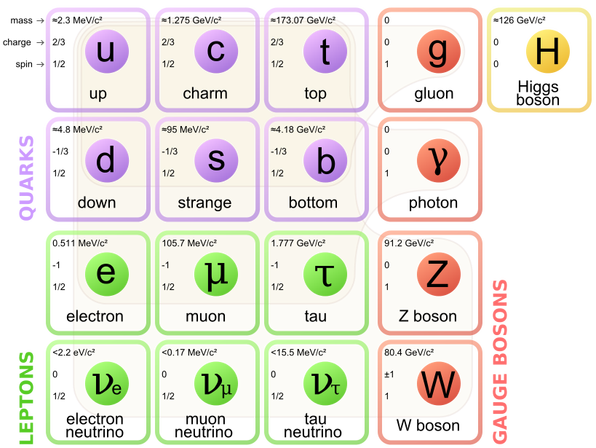
\includegraphics[scale=0.45]{the-standard-model.png}
\caption{Elementary particles of the Standard Model.}
\end{figure}
\\By leaving apart the gravitational interaction, every interaction is known to be mediated by a boson's exchange. The gauge sector is so composed of eight gluons which are the gauge bosons of SU(3)$_{c}$ and the $\gamma$, W$^{\pm}$ and Z$^0$ particles which are the four gauge bosons of \mbox{SU(2)$_{L}$ $\otimes$ U(1)$_{Y}$}. The gluons are massless, electrically neutral and carry color quantum number
\footnote{There are, in fact, eight gluons belonging to an SU(3) octet representation.}. The consequence of the gluons being colorful is that self-interaction terms will appear in the Lagrangian. The weak bosons W$^{\pm}$ and Z$^0$, where W$^{\pm}$ are charged $Q=\pm1$ respectively and Z$^0$ is electrically neutral, are massive and can self-interact as well as the gluons. The photon $\gamma$ is massless, chargeless and not self-interacting\cite{herrero1998standard}.
Actually, both the electromagnetic and the weak interaction are the manifestations at different energy scales of the same, much more fundamental, interaction: the electroweak interaction.

\section{Strong interactions}
The Quantum Chromodynamics (QCD) is the theory underlying the strong interaction. The QCD is a non-Abelian quantum gauge theory, based on the $SU(3)_c$ gauge group, acting on a degree of freedom called 'colour'. At very short wavelenghts it is essencially the theory of the free strongly interacting quarks and gluons, but at longer wavelenghts much more complex partonic bound states emerge, forming the colorless hadrons.
\\
The Lagrangian density describing QCD is 
\begin{equation}
\mathcal{L} = \bar{\psi_q^i}i\gamma^{\mu}(D_{\mu})_{ij}\psi_q^j - m_q\bar{\psi_q^i}\psi_{qi} - \frac{1}{4}F_{\mu\nu}^aF^{\mu\nu,a}
\end{equation}
where $\psi_q^i$ denotes a quark field with colour index i, $\psi_q = (\psi_q^R, \psi_q^G, \psi_q^B)^T$, and the covariant derivative responsible of the interactions is described by
\begin{equation}
(D_{\mu})_{ij} = \delta_{ij}\partial_{\mu} - ig_st_{ij}^aA_{\mu}^a
\end{equation}
The gauge fields $A_{\mu}^a$ coming from $(D_{\mu})_{ij}$ are 8 in total and they represent the eight colorfull gluon fields.
\\
Tipically, color is not present in the final state. Therefore, the fields describing particles will always contain the average over all possible incoming colours and sums over all possible outgoing colours\cite{Skands_2013}.
\\
The modern theory of the strong interactions, compared to its simple structure, shows lots of different features like colour confinement and asymptotic freedom, both due to the peculiar behaviour of the strong coupling constant $\alpha_s$.

\subsection{The running coupling constant in QCD}
The behaviour of the coupling constant is well determined by the evolution of the $\beta$ function, when the renormalization scale M is increased. This function comes from the Callan-Symanzik equation\cite{PhysRevD.2.1541, symanzik1970}
\begin{equation}
\left[ M \frac{\partial}{\partial M} + \beta(\lambda)\frac{\partial}{\partial \lambda} + n \gamma(\eta)\right]G^{(n)}(\{x_i\}; M, \lambda) = 0
\end{equation}
where $G^{(n)}(x_1,\cdots, x_n)$ stands for the \emph{n}-point Green's function and $\beta$ and $\gamma$ are two dimensionless parameters
\begin{equation}
\beta \equiv \frac{M}{\delta M}\delta{\lambda}\:; \hspace{1cm} \gamma \equiv - \frac{M}{\delta M}\delta \eta\:.
\end{equation}
It asserts that there exist two universal functions $\beta(\lambda)$ and $\gamma(\eta)$, related to the shifts of the coupling constant $\lambda$ and field strength $\eta$, that compensate for the shift of the Green's function in the renormalization scale $M$.
\\\\
Going more into details, the evolution of the $\beta$ function, giving the rate at which the renormalized coupling constant changes, determines the strength of the interaction and the conditions under which perturbation theory is valid.
\\
The calculation of Feynman diagrams at higher orders brings along with it some divergences in the matrix element, due to radiative corrections entering in the process. That issue is settled by the addition of some counterterms to subtract the ultraviolet divergences. Since Green's functions depend on $M$ through the counterterms, $\beta$ can be computed from the counterterms arising from the all possible corrections. Thus, at lower order,
\begin{equation}
\beta(g) = gM\frac{\partial}{\partial M}(-\delta_1+\delta_2+\tfrac{1}{2}\delta_3)\:.
\label{beta_function}
\end{equation}
Whether for Abelian quantum gauge theories the first two counterterms cancel each other leaving just the third, for non-Abelian quantum gauge theories, as QCD, all the counterterms get into the calculation with the convention
\\\\
\phantom{i}
\begin{figure*}[h]
\centering
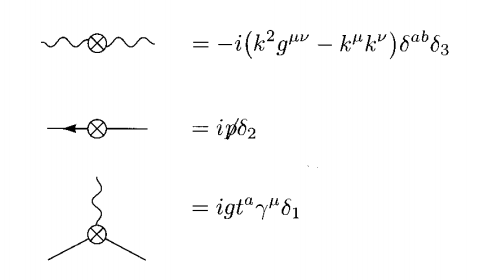
\includegraphics[scale=0.5]{counterterms.png}
\end{figure*}
\phantom{i}
\\\\
In order for the counterterms to cancel the divergences, from the computation of the radiative corrections at first order emerged that
\begin{align}
\begin{split}
\delta_1 &= - \frac{g^2}{(4\pi)^2}\frac{\Gamma(2-\frac{d}{2})}{(M^2)^{2-d/2}}[C_2(r)+C_2(G)] \\
\delta_2 &= - \frac{g^2}{(4\pi)^2}\frac{\Gamma(2-\frac{d}{2})}{(M^2)^{2-d/2}}C_2(r) \\
\delta_3 &= \frac{g^2}{(4\pi)^2}\frac{\Gamma(2-\frac{d}{2})}{(M^2)^{2-d/2}}\Bigl[\frac{5}{3}C_2(G)-\frac{4}{3}n_fC(r)\Bigr]
\end{split}
\label{counterterms}
\end{align}
where $C$ and $C_2$ are coefficients deriving from the group theory\footnote{Given a symmetry group G, the representation matrices in the irreducible rappresentation $r$ are $t_r^a$, generally known as \emph{generators}, which satisfy the commutation relation 
\begin{equation*}
\centering
[t^b;t^c]=if^{bcd}t^d \;.
\end{equation*}
As long as the generators are Hermitian, they satisfy the two relations
\begin{equation*}
tr[t_r^at_r^b] = C(r)\delta^{ab}; \hspace{0.3cm} f^{acd}f^{bcd} = C_2(G)\delta^{ab}
\end{equation*}
where $C_2(G)$ is the \emph{quadratic Casimir operator} of the adjoynt representation of the group.}, $M$ is the renormalization scale and $n_f$ is the fermion's number for the theory.
\\\\
Plugging the three counterterms of Eq.(\ref{counterterms}) into the $\beta$ function (Eq.(\ref{beta_function})), it turns out to be
\begin{equation}
\beta(g) = -\frac{g^3}{(4\pi)^2}\Bigl[\frac{11}{3}C_2(G)-\frac{4}{3}n_fC(r)\Bigr] \;.
\label{beta_function_final}
\end{equation}
In QCD with three colors, described by an $SU(3)$ gauge theory with fermions in the fundamental representation, Eq.(\ref{beta_function_final}) becomes
\begin{equation}
\beta(g) = -\frac{g^3}{(4\pi)^2}\Bigl[11-\frac{2}{3}n_f\Bigr] \;.
\end{equation}
The renormalized coupling constant obtained from the renormalization group equation\footnote{The \emph{renormalization group equation} permits to derive the renormalized coupling constant once computed $\beta$ frunction
\begin{equation*}
\frac{d}{d\mbox{log}(Q/M)}\bar{g} = \beta(\bar{g}) \;.
\end{equation*}} is
\begin{equation}
\alpha_s(Q) = \frac{\alpha_s}{1+(\frac{\alpha_s}{2\pi}[11-\frac{2}{3}n_f]\mbox{log}(k/M))}
\label{alpha_strong}
\end{equation}
It becomes easy to note how for a sufficiently small number $n_f$ of fermions, QCD becomes \emph{asymptotycally free}, because the strong coupling constant in Eq.(\ref{alpha_strong}) tends to zero at large momenta. On the other hand, $\alpha_s$ increase exponentially as momentum transfert decrease, exhibiting the \emph{color confinement} phenomenon \cite{Peskin:1995ev}.
\begin{figure}[t]
\centering
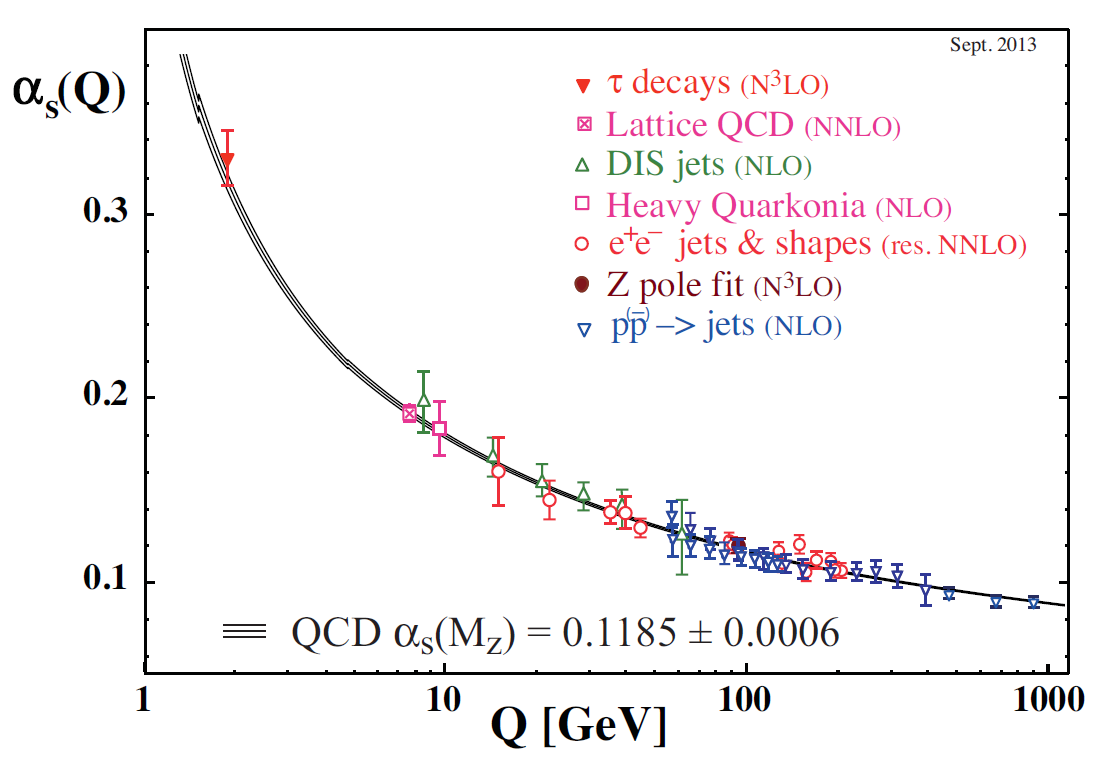
\includegraphics[scale=0.3]{QCD-running-coupling.png}
\caption{The plot shows the behaviour of the strong coupling constant $\alpha_s$, as a function of the transfer momentum $Q$. }
\end{figure}

\subsection{Hard hadronic scattering and the proton structure}
The main difference between leptons and hadrons, making the study of the latter of wide interest, lies in the fact that hadrons are not elementary particles, but have a structure containing colorless combinations of valence quarks plus virtual pairs of quarks/anti-quarks known as \emph{sea quarks}. Sea quarks arise from gluon splitting; a pair of quarks can in turn annihilate producing a gluon. In addition, gluons are present in the sea also owing to the three-gluon and four-gluon vertices.
\\
Colliding hadrons, protons more precisely, becomes a quite hard process to describe as energy is increased. After a certain threshold, in fact, the proton breaks up, manifesting his complex internal structure and making the scattering of the constituent quarks and gluons possible, such as $qq$, $q\bar{q}$, $gq$, $g\bar{q}$, $gg$.
\\
In proton collisions, being the elementary interaction at parton level, each of the scattering constituents carries a different fraction \emph{x} of the proton four-momentum, known as Bjorken's scaling variable \cite{altarelli2013collider}. The rescaled center-of-mass energy, taking into consideration the fraction \emph{x} of both partons, turns out to be $\sqrt{\hat{s}}=\sqrt{x_1x_2s}$, where $s$ is the center-of-mass energy of the incoming protons and $x_1$ and $x_2$ represent the fraction of the momentum carried by each of the interacting partons. With this interpretation, the cross section describing a typical $pp \rightarrow X$ process has to include a term that describes the partonic hard scattering, calculated using perturbative Quantum Field Theory, and factors for the incoming flux of partons, the \emph{parton distribution functions} (PDF).
\\
Considering that, the cross section for a typical $pp$ collision takes the form
\begin{equation}
\sigma(pp \rightarrow X) = \displaystyle\sum_{i,j} \int dx_1 \int dx_2f_i(x_1,\mu_F^2)f_j(x_2,\mu_F^2)\cdot\hat{\sigma}_{ij \rightarrow X}(x_1x_2s,\mu_R^2, \mu_F^2)
\label{pp_cross_section}
\end{equation}
In Eq.(\ref{pp_cross_section}) the sum runs over all possible initial-state partons, with longitudinal momentum $x_{1,2}$, that can give rise to a final state $X$ at a center-of-mass energy of $\sqrt{x_1x_2s}$ \cite{Butterworth_2012}. The \emph{factorization scale} parameter $\mu_F$ represent the scale at which the separation between the hard perturbative interaction and the long distance non-perturbative evolution of the produced partons occurs.The $\hat{\sigma}_{i,j \rightarrow X}$ term describes the elementary partonic cross section at the scale $\mu_F$ and $\mu_R$, where $\mu_R$ is the \emph{renormalization scale}, introduced in perturbative QCD to cut ultraviolet divergences. The two terms $f_i(x_1,\mu_F^2)$ and $f_j(x_2,\mu_F^2)$ are the PDFs of each parton involved into the process and describe the probability density for a parton to be found within the incoming pronton and to carry a certain fraction of its momentum.
\\
Since QCD doesn't predict the parton content of the proton, the shapes of the PDFs are obtained by a fit to data at different scales $Q^2$ in various processes, using the DGLAP evolution equations \cite{ALTARELLI1977298}. Introducing the variable $\tau = \ln(Q^2/\mu^2)$ and denoting the gluon distribution function in the nucleon by $g(x,\tau)$ and that of the quark by $q(x,\tau)$, the formula to derive the quark distribution functions, including the gluon splitting effect too, can be written as \cite{nagashima2010elementary}
\begin{equation}
\frac{dq(x,\tau)}{d\tau} = \frac{\alpha_s}{2\pi}\int_x^1\frac{dy}{y}\Bigl[q(y,\tau)P_{q\leftarrow q}\Bigl(\frac{x}{y}\Bigr)+g(y,\tau)P_{q\leftarrow g}\Bigl(\frac{x}{y}\Bigr)\Bigr]
\end{equation}
where $P_{a\leftarrow b}$ are the splitting functions for the parton $a$ to emit the parton $b$.
\\ 
Similarly, the gluon distribution function can be derived using
\begin{equation}
\frac{dg(x,\tau)}{d\tau} = \frac{\alpha_s}{2\pi}\int_x^1\frac{dy}{y}\Bigl[q(y,\tau)P_{g\leftarrow q}\Bigl(\frac{x}{y}\Bigr)+g(y,\tau)P_{g\leftarrow g}\Bigl(\frac{x}{y}\Bigr)\Bigr]
\end{equation}
These kind of equations permit to determine the behavior of the flux of gluons and quarks within the proton in terms of PDFs at all values of $Q^2$, above the input scale $Q_0^2$ at which they are parametrized as a function of $x$.
\\
In Figure \ref{pdf} you can see how, for big momentum fractions (large $x$-values) the main contributions come from $u$ and $d$ quarks, with about a 2:1 ratio, while other flavours are virtually absent
\footnote{In this way, we can consider the proton made of two $up$-quarks and one $down$-quark.}.
With momentum decreasing, the contribution of the other flavours different from $u$ and $d$, generated from the $g \rightarrow qq$ splitting starts also to increase.
\\
At low energies the main contribution to the parton flux comes from the gluons
\footnote{Notice how in Figure \ref{pdf} the gluons distribution is scaled down by a $1/10$ factor, so its contribution is extremely high compared to the one coming from the various quarks.}
and this feature is further accentuated by increasing the $Q^2$ scale.
\begin{figure}[t]
\centering
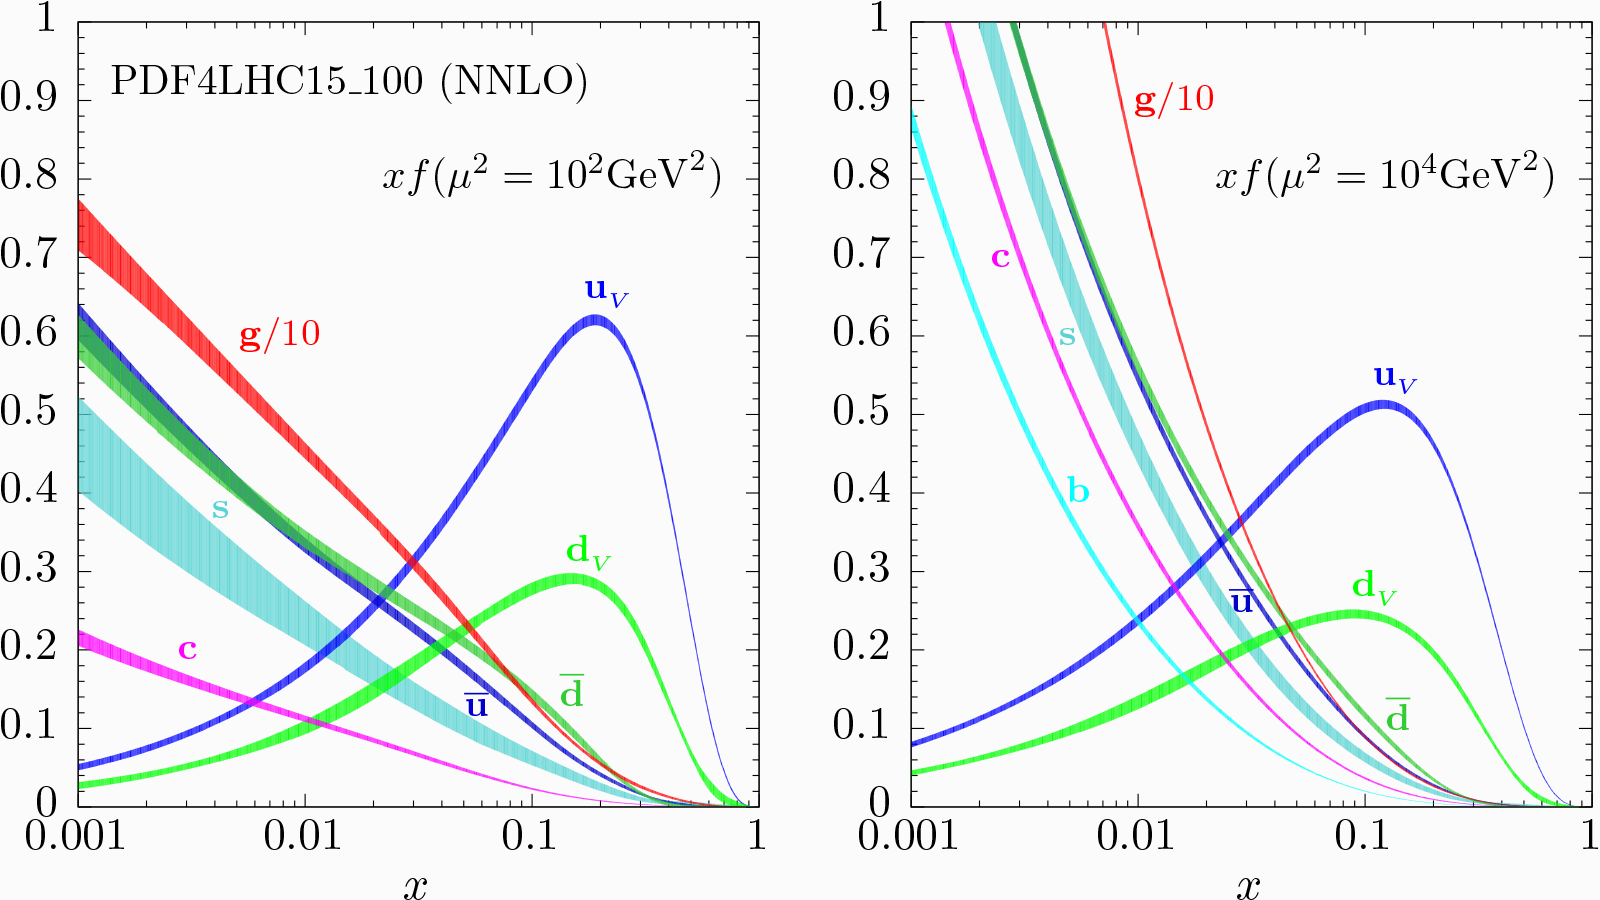
\includegraphics[scale=0.22]{pdf.png}
\caption{PDF's $x$ dependencies on a logarithmic scale for two different energy scales. On the left a "low" scale, while on the the right an "high" scale, typical from LHC, are presented. }
\label{pdf}
\end{figure}

\section{Electroweak interactions}
\emph{<<Leptons interact only with photons and with the intermediate bosons that presumably mediate weak interactions. What could be more natural than to unite these spin-one bosons
into a multiplet of gauge fields?>>} (S. Weinberg, 1967)\cite{PhysRevLett.19.1264}.
\\\\
The electroweak theory is an \mbox{SU(2)$_L$ $\otimes$ U(1)$_Y$} local gauge theory, where SU(2)$_L$ group only left-handed particles and refers to the weak isospin charge $I$, while U(1)$_Y$ is related to the weak hypercharge $Y$, both connected together by the equation:
\begin{equation}
Y = 2(Q-I_3)
\end{equation}
Due to the nature of the theory, its Lagrangian needs to be invariant under \mbox{SU(2) $\otimes$ U(1)} global gauge transformations.
The electroweak Lagrangian which involve only gauge bosons, fermions and their interactions turns out to be
\begin{align}
\begin{split}
\mathcal{L} = - \frac{1}{4} \displaystyle\sum_{A=1}^3F_{\mu\nu}^AF^{A\mu\nu} - \frac{1}{4} B_{\mu\nu}&B^{\mu\nu} + \\ 
 + \bar{\psi}_Li&\gamma^{\mu}D_{\mu}\psi_L + \bar{\psi}_Ri\gamma^{\mu}D_{\mu}\psi_R
 \end{split}
\label{EW_lagrangian}
\end{align}
where the gauge fields $B_{\mu\nu}$ and $F_{\mu\nu}^A$ are
\begin{align}
\begin{split}
&B_{\mu\nu} = \partial_{\mu}B_{\nu} - \partial_{\nu}B_{\mu} \\
&F_{\mu\nu}^A = \partial_{\mu}W_{\nu}^A - \partial_{\nu}W_{\mu}^A - g\epsilon_{ABC}W_{\mu}^BW_{\nu}^C
\end{split}
\end{align}
and $D_{\mu}$ is the covariant derivatives for the gauge group, usefull to introduce the interactions in the Lagrangian (\ref{EW_lagrangian}) and making it invariant under local gauge transformations:
\begin{equation}
D^{\mu} = \partial^{\mu} + ig \boldsymbol{\tau} \cdot \hat{\boldsymbol{W}}^{\mu} /2+ig'\hat{B}^{\mu} /2
\end{equation}
where $\boldsymbol{\tau} = (\tau_1, \tau_2, \tau_3)$ are the Pauli matrices and $\hat{\boldsymbol{W}}^{\mu} = (\hat{W}_1^{\mu}, \hat{W}_2^{\mu}, \hat{W}_3^{\mu})$ stands for the three generators of the SU(2)$_L$ group. 
\\
The four gauge fields coming from the generators of the group cannot be considered as the physical electroweak gauge bosons, because of the mass issue: the four gauge fields are all massless, while in the physical ones the three weak bosons $W^{\pm}$ and $Z^0$ are actually massive
\footnote{($m_W = 80.370 \pm 0.019$ GeV, $m_Z = 91.187 \pm 0.007$ GeV) \cite{Aaboud_2018, Arnaudon}}\cite{altarelli2000standard}.
The physical bosons come up from the symmetry-breaking mechanism, discussed further below, through a mixing between the unphysical fields
\begin{align}
\begin{split}
&W_{\mu}^{(\pm)} = \frac{1}{\sqrt{2}}(W_{\mu}^1 \pm iW_{\mu}^2) \\
&Z_{\mu}^0 = cos\theta_W W_{\mu}^3 + sin\theta_W B_{\mu} \\
&A_{\mu} = -sin\theta_W W_{\mu}^3 + cos\theta_W B_{\mu} 
\end{split}
\label{EWbosons}
\end{align}
The fields in (\ref{EWbosons}) are in fact the physical particle fields, where $W_{\mu}^{\pm}$ stand for the electrically charged weak interacting bosons, $Z_{\mu}^0$ represents the electrically neutral weak interacting boson and $A_{\mu}$ denote the photon, the only field left massless after the symmetry-breaking process\cite{Weinberg:1996kr}.
\\ \\
The Feynman rules of the theory show several vertices between bosons and fermions, in addition to some self-interacting vertices between the gauge bosons, due to the non-Abelianity of \mbox{$SU(2)_L \otimes U(1)_Y$}.

\begin{figure}[h]
\centering
\subfloat{\feynmandiagram [small, horizontal=e to f] {
  e -- [boson, edge label = \small$\gamma$, near start]  f,
  h [particle =$f$] -- [fermion] f -- [fermion] i[particle=$f$],
};} \hspace{0.5cm}
\subfloat{\feynmandiagram [small, horizontal=e to f] {
  e -- [boson, edge label = \small$W$, near start]  f,
  h [particle =$\nu_l$] -- [fermion] f -- [fermion] i[particle=$l$],
};} \hspace{0.5cm}
\subfloat{\feynmandiagram [small, horizontal=e to f] {
  e -- [boson, edge label = \small$W$, near start]  f,
  h [particle =$q_i$] -- [fermion] f -- [fermion] i[particle=$q_j$],
};} \hspace{0.5cm}
\subfloat{\feynmandiagram [small, horizontal=e to f] {
  e -- [boson, edge label = \small$Z$, near start]  f,
  h [particle =$f$] -- [fermion] f -- [fermion] i[particle=$f$],
};} \\ \vspace{0.5cm}
\subfloat{\feynmandiagram [small, horizontal=e to f] {
  e -- [boson, edge label = \small$\gamma/Z$, near start]  f,
  h -- [boson, edge label=\small$W$, near start] f -- [boson, edge label=$\small{W}$, near end] i,
};} \hspace{0.5cm}
\subfloat{\feynmandiagram [small, horizontal=i1 to f2] {
  i1 -- [boson, edge label=\small$W$, near start] c -- [boson, edge label=\small$W$, near end] f1,
  i2 -- [boson, edge label=\small$W$, near start] c -- [boson, edge label=\small$W$, near end] f2,
};}\hspace{0.5cm}
\subfloat{\feynmandiagram [small, horizontal=i1 to f2] {
  i1 -- [boson, edge label=\small$W$, near start] c -- [boson, edge label=\small$\gamma/Z$, near end] f1,
  i2 -- [boson, edge label=\small$\gamma/Z$, near start] c -- [boson, edge label=\small$W$, near end] f2,
};}\\\hspace{0.3cm}
\caption{The Feynman vertices for the electroweak interaction. On the top the fermions couplings are displayed, while on the bottom the self-interacting couplings are shown.}
\end{figure}

\subsection{The Higgs Field and the Mechanism}
The \emph{Higgs mechanism} is essential to explain how gauge vector bosons acquire mass through a spontaneous symmetry breaking
\footnote{The \emph{spontaneous symmetry breaking} describes systems where the lowest energy vacuum solutions do not exhibit the same symmetry of the Lagrangian. In these vacuum solutions, the symmetry is broken for perturbations around them even though the entire Lagrangian retains that symmetry.}
. Without this mechanism, in fact, all bosons would be considered massless and this doesn't reflect the experimental evidences. 
\\\\
The main difference between a vector massive field and a massless one lies in the number of degrees of freedom, three in the former case, two in the latter in particular. This discrepancy indicates that some additional fields must be present in order to give mass to the originally massless gauge bosons.
\\\\
The fundamental idea presented by Higgs is to assume that a "hidden" field has to exists, whose potential's ground state, shown in Figure \ref{mexican_hat}, breaks the Lagrangian symmetry spontaneously \cite{Aitchison_Hey}.
\\
That field, known as the \emph{Higgs field}, permeates every region of the Universe. At temperatures high enough, all particles are massless and the symmetry is unbroken. Once a critical temperature is reached, typically shortly after the hot big bang, the Higgs field develops a vacuum expectation value (VEV) different from $0$
\footnote{The \emph{vacuum expectation value} of a field is the lowest-energy configuration that satisfies the classical equations of motion \cite{Schwartz:2013pla}.} and so the symmetry breaks up, giving masses to the particles, both bosons and fermions, through the Higgs boson interactions.
\begin{figure}[t]
\centering
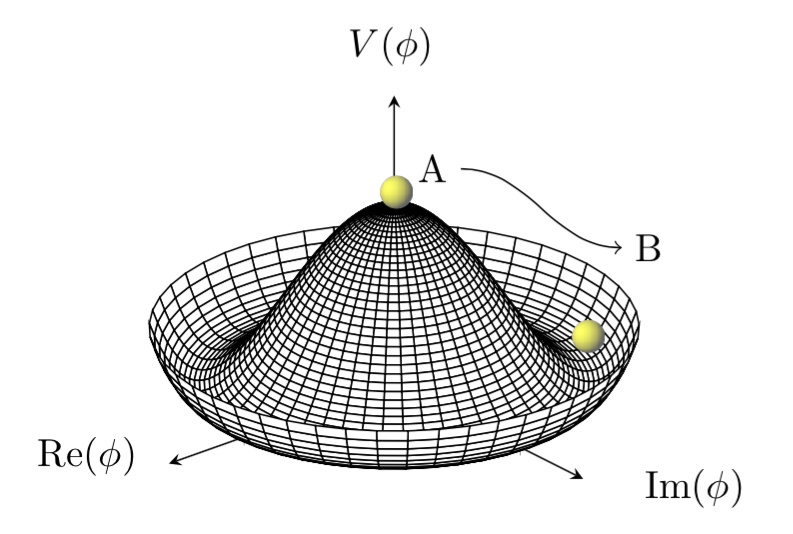
\includegraphics[scale=0.36]{higgs_potential.png}
\caption{Graphical representation of the Higgs potential $V(\phi)$, usually known as "mexican hat" potential. The point A is the high energy symmetric local maximum, while the point B is the low energy asymmetric local minimum. The symmetry breaks up once a particle flows from A to B, choosing a particular local minimum among the continuum set of low energy minima.}
\label{mexican_hat}
\end{figure}
The geometric structure of the Higgs field is an $SU(2)$ doublet, which is a scalar under Lorentz transformations, and under $U(1)$ rotations, it is multiplied by a phase.
\\
The four degrees of freedom so introduced are the real actors of the mass generation: three out of four of them mix with the originally massless vector bosons and the only single remaining degree of freedom becomes the new scalar Higgs boson.
\\\\
From the quantitative point of view, the simplest choice for a field with at least the three necessary degrees of freedom for the success of the mechanism is a complex $SU(2)$ doublet of scalar fields $\hat{\phi}$
\begin{equation}
\hat{\phi} = \begin{pmatrix}
\hat{\phi}^+ \\ \hat{\phi}^0 
\end{pmatrix} \text{,} \hspace{0.4cm} Y_{\phi}=+1
\end{equation}
described by the Lagrangian
\begin{equation}
\hat{\mathcal{L}}_{\phi} = (\partial_{\mu}\hat{\phi}^\dag)(\partial^{\mu}\hat{\phi})+\mu^2\hat{\phi}^\dag\hat{\phi}-\frac{\lambda}{4}(\hat{\phi}^\dag\hat{\phi})^2
\label{Higgs_lagrangian}
\end{equation}
This Lagrangian is invariant under $SU(2)$ and $U(1)$ global transformations. To make it invariant under local transformations too, you need to introduce three gauge fields for the $SU(2)$ group ($\hat{W}_i^{\mu}(x)$ with $i=1,2,3$) and the $\hat{B}^{\mu}(x)$ field for the group $U(1)$. 
\\
These additions can be inserted by the use of the covariant derivative
\begin{equation}
\hat{D}^{\mu} \hat{\phi} = (\partial^{\mu} + ig \boldsymbol{\tau} \cdot \hat{\boldsymbol{W}}^{\mu} /2+ig'\hat{B}^{\mu} /2)\hat{\phi}
\end{equation}
where $\boldsymbol{\tau} = (\tau_1, \tau_2, \tau_3)$ is the three Pauli matrices set.
\\\\
The Lagrangian for the Higgs sector consisting of the gauge fields and the Higgs fields (without gauge-fixing ang ghost terms) so becomes
\begin{align}
\hat{\mathcal{L}}_{G\phi} = &(\hat{D}_{\mu}\hat{\phi})^{\dag}(\hat{D}^{\mu}\hat{\phi})+\mu^2\hat{\phi}^{\dag}\hat{\phi}-\frac{\lambda}{4}(\hat{\phi}^{\dag}\hat{\phi})^2 \\
&-\frac{1}{4}\hat{\boldsymbol{F}}_{\mu\nu}\cdot\hat{\boldsymbol{F}}^{\mu\nu}-\frac{1}{4}\hat{G}_{\mu\nu}\hat{G}^{\mu\nu}
\label{Higgs_local_invariant}
\end{align}
where $\hat{\boldsymbol{F}}_{\mu\nu}$ is the $SU(2)$ field strength tensor for the gauge fields $\hat{\boldsymbol{W}}^{\mu}$ and $\hat{G}_{\mu\nu}$ is the $U(1)$ field strength tensor for the gauge field $\hat{B}^{\mu}$ respectively given by
\begin{align}
\hat{\boldsymbol{F}}^{\mu\nu}& \hspace{0.1cm}=\hspace{0.1cm} \partial^{\mu}\hat{\boldsymbol{W}}^{\nu}-\partial^{\nu}\hat{\boldsymbol{W}}^{\mu}-g\hat{\boldsymbol{W}}^{\mu}\times\hat{\boldsymbol{W}}^{\nu} \\
\hat{G}^{\mu\nu}& \hspace{0.1cm}=\hspace{0.1cm} \partial^{\mu}\hat{B}^{\nu}-\partial^{\nu}\hat{B}^{\mu}
\end{align}
The plus sign in the $\mu^2$ term in the Eq.(\ref{Higgs_lagrangian}) and in Eq.(\ref{Higgs_local_invariant}) reflects the symmetry breaking. That particular choice for the sign creates the typical shape visible in Figure \ref{mexican_hat}, and allows the field $\phi(x)$ to acquire a vacuum expectation value at the minimum of the potential
\begin{equation}
\langle\phi\rangle_0 \equiv \langle0|\phi|0\rangle = \begin{pmatrix} 
		0 \\ 
		\frac{v}{\sqrt{2}} 
		\end{pmatrix} \hspace{0.4cm} \text{with} \hspace{0.4cm} v = \Bigl(-\frac{\mu^2}{\lambda}\Bigr)^{1/2}
\label{vev}
\end{equation}
It's now time to apply perturbation theory, expanding around one of the minima $v$ by defining the physical Higgs field $\hat{H}$ and parametrizing $\hat{\phi}$ as
\begin{equation}
\hat{\phi} = \begin{pmatrix} 
		0 \\ 
		\frac{1}{\sqrt{2}}(v+\hat{H}) 
		\end{pmatrix}
\label{expansion}
\end{equation}
Inserting Eq.(\ref{expansion}) in the local gauge invariant Lagrangian and making the symmetry breaking manifest, the free fields quadratic parts of Eq.(\ref{Higgs_local_invariant}) can be written as
\begin{align}
\begin{split}
\hat{\mathcal{L}}^{free}_{G\phi} \hspace{0.2cm} =& \hspace{0.4cm} \frac{1}{2}\partial_{\mu}\hat{H}\partial^{\mu}\hat{H}-\mu^2\hat{H}^2 \\
& -\frac{1}{4}(\partial_{\mu}\hat{W}_{1\nu}-\partial_{\nu}\hat{W}_{1\mu})(\partial^{\mu}\hat{W}_1^{\nu}-\partial^{\nu}\hat{W}_1^{\mu}) + \frac{1}{8}g^2v^2\hat{W}_{1\mu}\hat{W}_1^{\mu} \\
& -\frac{1}{4}(\partial_{\mu}\hat{W}_{2\nu}-\partial_{\nu}\hat{W}_{2\mu})(\partial^{\mu}\hat{W}_2^{\nu}-\partial^{\nu}\hat{W}_2^{\mu}) + \frac{1}{8}g^2v^2\hat{W}_{2\mu}\hat{W}_2^{\mu} \\
& -\frac{1}{4}(\partial_{\mu}\hat{Z}_{\nu}-\partial_{\nu}\hat{Z}_{\mu})(\partial^{\mu}\hat{Z}^{\nu}-\partial^{\nu}\hat{Z}^{\mu}) + \frac{1}{8}g^2v^2\hat{Z}_{\mu}\hat{Z}^{\mu} \\
& -\frac{1}{4}\hat{F}_{\mu\nu}\hat{F}^{\mu\nu}
\end{split}
\label{expanded_lagrangian}
\end{align}
in unitary gauge
\footnote{The \emph{unitary gauge} or unitarity gauge is a particular choice of a gauge fixing in a gauge theory with a spontaneous symmetry breaking. In this gauge, the scalar field $\phi$ responsible for the Higgs mechanism are transformed into a basis in which their Goldstone boson components are set to zero. Writing the field $\phi$ in terms of four fields $\hat{\theta}_{1,2,3}(x)$ and $H(x)$, the unitary gauge allows to rewrite it as
\footnotesize
\begin{equation*}
\hat{\phi} = \begin{pmatrix} 
		\hat{\theta_2} + i\hat{\theta_1} \\ 
		\frac{1}{\sqrt{2}}(v+\hat{H}) - i\hat{\theta_3} 
		\end{pmatrix}
		= \exp^{i\theta_a(x)\tau^a(x)/v}\begin{pmatrix} 
		0 \\ 
		\frac{1}{\sqrt{2}}(v+\hat{H}) 
		\end{pmatrix}
\end{equation*}
making the manifest number of scalar degrees of freedom minimal.}
, where
\begin{align}
\hat{F}^{\mu\nu} =& \hspace{0.1cm} \partial^{\mu}\hat{A}^{\nu} - \partial^{\nu}\hat{A}^{\mu} \\
\hat{Z}^{\mu} =& \hspace{0.1cm} \cos{\theta}_W\hat{W}_3^{\mu} - \sin{\theta}_W\hat{B}^{\mu} \\
\hat{A}^{\mu} =& \hspace{0.1cm} \sin{\theta}_W\hat{W}_3^{\mu} + \cos{\theta}_W\hat{B}^{\mu}
\end{align}
with
\begin{equation}
\cos{\theta}_W = \frac{g}{\sqrt{g^2+g'^2}} \hspace{0.2cm} \text{,} \hspace{0.4cm} \sin{\theta}_W = \frac{g'}{\sqrt{g^2+g'^2}}
\end{equation}
In Eq.(\ref{expanded_lagrangian}) it's easy to see how, after the spontaneous symmetry breaking due to the vacuum expectation value, the mass terms for the physical gauge bosons appear as well as for the Higgs boson itself
\footnote{Both charged weak interacting bosons $W$s have the same mass term, while the only field left massless after the symmetry breaking remains the photon field, as it should be.}.
From terms which are bilinear in the fields $\hat{W}_1^{\mu}$, $\hat{W}_2^{\mu}$, $\hat{Z}^{\mu}$ you can derive the explicit form for the masses of the particles
\begin{equation}
m_H = \sqrt{2} \mu = \frac{\sqrt{\lambda}v}{\sqrt{2}} \text{,} \hspace{0.4cm} m_W = \frac{gv}{2} \text{,} \hspace{0.4cm} m_Z = \frac{m_W}{\cos{\theta}_W} 
\end{equation}
In a similar way as the one seen for bosons, also for the fermionic sector of the Higgs interaction Lagrangian is possible to give mass to fermions, without introducing an explicit mass term in the Lagrangian. Using electrons as an example, it could be assumed an hypothetical coupling between an electron-type SU(2) doublet
\begin{equation}
\begin{pmatrix}
\nu_{e} \\ e^- 
\end{pmatrix}_L \hspace{0.2cm} \text{,}
\end{equation}
the Higgs doublet $\phi$ and the R-component of the electron field preserving the SU(2)$_L$ invariance, feature required by the electroweak interaction nature. The Lagrangian for these kinds of couplings, usually known as \emph{Yukawa couplings}, can be written as 
\begin{equation}
\mathcal{\hat{L}}_{\text{int}} = \lambda_e\Bigl(\bar{\hat{l}}_{eL}\hat{\phi} \hat{e}^-_R + \hat{\phi}^{\dag}\hat{e}^-_R\hat{l}_{eL}\Bigr)
\label{lepton_lagrangian}
\end{equation}
where $\lambda_e$ is the self-coupling of the fermion, an electron in this case and it is an arbitrary parameter of the theory.Expanding the Lagrangian (\ref{lepton_lagrangian}) around a minimum of the Higgs field, it turns out to be
\begin{align}
\begin{split}
\mathcal{\hat{L}}_{\text{Yukawa}} =& \frac{\lambda_ev}{\sqrt{2}}\Bigl(\bar{\hat{e}}^-_L\hat{e}^-_R + \bar{\hat{e}}^-_R\hat{e}^-_L\Bigr) + \frac{\lambda_e}{\sqrt{2}}\Bigl(\bar{\hat{e}}^-_L\hat{e}^-_R + \bar{\hat{e}}^-_R\hat{e}^-_L\Bigr)\hat{H} \\
=& m_e\bar{\hat{e}}\hat{e} + \frac{m_e}{v}\bar{\hat{e}}\hat{e}\hat{H} \hspace{0.4cm} \text{.}
\end{split}
\label{lepton_expanded}
\end{align}
The first term of the Lagrangian (\ref{lepton_expanded}) is exactly the Dirac mass term for the electron, making easy to recognise
\begin{equation}
m_e = \lambda_ev/\sqrt{2}
\end{equation}
It seeks to identify the last term of the Lagrangian (\ref{lepton_expanded}) as a coupling between the electron Higgs fields, implying also no neutrino-Higgs interactions, due to the absence of $\nu_R$ component for the neutrinos field.
\\\\
It is possible to repete this mass generation mechanism for each fermion in the theory and so derive the values for the different masses, as functions of the arbitrary self-coupling of the selected fermion
\begin{equation}
m_f = \lambda_fv/\sqrt{2} \hspace{0.4cm} \text{.}
\end{equation}
In this way the masses are included in the Standard Model, but they are not predicted, thus they must be measured.
\\\\
The Higgs boson interacts with fermions with a strength proportional to their mass $m_f$, therefore it couples more strongly to the heaviest fermions.
\\
Notice how, with the same isodoublet $\hat{\phi}$ of scalar fields, the Higgs mechanism allows to generate the masses for fermions and weak interacting vector bosons $W^\pm$, $Z^0$ leaving massless the photon field, while preserving the \mbox{$SU(2) \times U(1)$} gauge symmetry, which is now hidden by the spontaneous symmetry breaking \cite{Aitchison_Hey, Djouadi_2008}.

\subsection{Higgs boson in the Standard Model}
The massive particle arising from the spontaneously symmetry breaking, known as the \emph{Higgs boson}\cite{PhysRevLett.13.321, PhysRevLett.13.508}, is well described in the first line of Eq.(\ref{expanded_lagrangian}) Lagrangian. The kinetic term, $\frac{1}{2}\partial_{\mu}\hat{H}\partial^{\mu}\hat{H}-\mu^2\hat{H}^2$, comes from the term involving the covariant derivative $|D_{\mu}\phi|^2$, while the mass term derives from the structure of the Higgs potential.
\\
After the vacuum expansion, the terms concerning the mass and the intercations for the Higgs boson in the Lagrangian are
\begin{equation}
\hat{\mathcal{L}}^{int}_{G\phi} \hspace{0.2cm} = \hspace{0.2cm} -\lambda v^2\hat{H}^2 -\lambda v\hat{H}^3 -\frac{\lambda}{2!}\hat{H}^4 
\label{interactions}
\end{equation}
From Eq.(\ref{interactions}) you can see how the particle's mass turns out to be simply as 
\begin{equation}
M_H^2 = 2\lambda v^2 = -2\mu^2
\end{equation}
and the Feynman rules for the Higgs self-interaction vertices (Figure \ref{self_H}) are given by
\begin{equation}
g_{H^3} = (3!)i\lambda v = 3i\frac{M_H^2}{v} \hspace{0.2cm} \text{,} \hspace{0.4cm} g_{H^4} = (4!)i\frac{\lambda}{4} = 3i\frac{M_H^2}{v^2}
\end{equation}
The interaction with gauge bosons and fermions are described by the Higgs boson couplings
\begin{equation}
g_{Hff} = i\frac{m_f}{v} \hspace{0.2cm} \text{,} \hspace{0.4cm} g_{HVV} = -2i\frac{M_V^2}{v} \hspace{0.2cm} \text{,} \hspace{0.4cm} g_{HHVV} = -2i\frac{M_V^2}{v^2}
\end{equation}
The vacuum expectation value for the Higgs field, seen in Eq.(\ref{vev}), is fixed in terms of the $W$ boson mass $M_W$
\begin{equation}
M_W = \frac{1}{2}gv \hspace{0.2cm} \Rightarrow \hspace{0.2cm} v = \frac{2M_W}{g} \simeq \text{246 GeV}
\end{equation}
\begin{figure}[h]
\centering
\subfloat[][]{\feynmandiagram [horizontal=e to f] {
  e -- [scalar, edge label = \small$H$, near start]  f,
  h -- [scalar, edge label = \small$H$, near start] f -- [scalar, edge label = \small$H$, near end] i,
};} \hspace{0.8cm}
\subfloat[][]{\feynmandiagram [horizontal=i1 to f2] {
  i1 -- [scalar, edge label=\small$H$, near start] c -- [scalar, edge label=\small$H$, near end] f1,
  i2 -- [scalar, edge label=\small$H$, near start] c -- [scalar, edge label=\small$H$, near end] f2,
};}
\caption{a)Three-line Higgs self-interacting vertex, b)Four-line Higgs self-interacting vertex.}
\label{self_H}
\end{figure}

\section{The Higgs sector at LHC}
\emph{<<This summer I have discovered something totally useless.>>} (P. W. Higgs, 1964)
\\ \\
In this section the Higgs boson sector will be presented. Starting from the various production modes, it continue with the different decay channels, focusing on $H \rightarrow \gamma \gamma$, which is the channel investigated in this work.
\subsection{Higgs boson production modes}
Being the LHC a proton-proton collider, the main process contributing to the Higgs boson production must contain gluons deriving from the colliding protons.
In order of decreasing cross section, the channels involved into the Higgs production are:
\begin{itemize}
\item \emph{Gluon fusion} (ggH): the most common production mode at LHC over the whole mass spectrum, due to the proton structure. It leads to about 85\% of the total cross section in the mass range of 120-130 GeV. This kind of process requires the fusion of two gluons, producing the Higgs boson through a heavy quark loop, tipically a top quark, because of its heavy mass.
\begin{figure}[H]
\centering
\feynmandiagram [small, horizontal=g1 to t1] {
  g1 --[gluon, edge label=\small$g$] t1 -- [fermion] t2 --[fermion] t3 --[fermion] t1,
  g2 --[gluon, edge label=\small$g$] t2,
  t3 -- [scalar, edge label = \small$H$]  h,
  g1 --[opacity=0] g2,
};
\end{figure}
\item \emph{Vector Boson Fusion} (VBF): this production mode is the second most dominant in the Higgs sector and is the responsible of around 7\% of the total number of Higgs produced in the selected mass range. It consists in the scattering of two incoming quarks, each of them emitting a $W^{\pm}$ or $Z^0$ boson which, in turn, interact to produce the Higgs boson. The peculiar signature of this production is the presence of two high-energy forward jets, arising from the scattered valence quarks of the two protons.
\begin{figure*}[h]
\centering
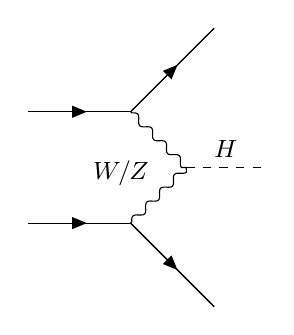
\begin{tikzpicture}
  \begin{feynman} [small]
  	\vertex (i1);
  	\vertex[right=1.3cm of i1] (v1);
  	\vertex[above right=1.5cm of v1] (f1);
  	\vertex[below right=of v1] (v2);
  	\vertex[right=of v2] (h);
  	\vertex[below left=of v2] (v3);
  	\vertex[left=1.3cm of v3] (i2);
  	\vertex[below right=1.5cm of v3] (f2);
  	
  	\diagram* {
  		(i1) -- [plain, fermion] (v1) -- [plain, fermion] (f1),
  		(i2) -- [plain, fermion] (v3) -- [plain, fermion] (f2),
  		(v1) -- [boson] (v2),
  		(v3) -- [boson, edge label=\small $W/Z$] (v2),
  		(v2) --[scalar, edge label = \small $H$] (h),
  		};
  	\end{feynman}
\end{tikzpicture}
\end{figure*}
\item \emph{Higgsstrahlung} (VH): even if the cross section for this production mode is comparable with the VBF cross section for masses between 120 and 130 GeV. The Higgs boson is emitted with an associated vector boson from a $W^{\pm}$ or $Z^0$ arising from two incoming quarks.
\begin{figure*}[h]
\centering
\feynmandiagram [small, horizontal=a to b] {
i1 -- [fermion] a -- [fermion] i2,
a -- [boson, edge label=\small$W/Z$] b,
f1 -- [boson] b -- [scalar, edge label= \small $H$] f2,
};
\end{figure*}
\item \emph{Top quark associated production} ($t\bar{t}H$): this particular production mode derive from two gluon splitting into two pairs of t-quarks. Just after it, two out of the four produced quarks interact emitting a Higgs boson, while the other two t-quarks will decay\footnote{The t-quark is the only quark which decays instead of hadronize. Because of its huge mass, the t-quark has an extremely short lifetime, predicted in $5 \times 10^{-25} \text{s}$. In this short amount of time the hadronisation process cannot take place and the t-quark decays as a "bare" quark.}
\begin{figure*}[!h]
\centering
\begin{tikzpicture}
  \begin{feynman} [small]
  	\vertex (i1);
  	\vertex[right=1.3cm of i1] (v1);
  	\vertex[above right=1.5cm of v1] (f1);
  	\vertex[below right=of v1] (v2);
  	\vertex[right=of v2] (h);
  	\vertex[below left=of v2] (v3);
  	\vertex[left=1.3cm of v3] (i2);
  	\vertex[below right=1.5cm of v3] (f2);
  	
  	\diagram* {
  		(i1) -- [gluon] (v1) -- [fermion, edge label = \small $t$] (f1),
  		(i2) -- [gluon] (v3)
  		(f2) -- [fermion, edge label = \small $\bar{t}$] (v3),
  		(v1) -- [fermion] (v2),
  		(v3) -- [fermion] (v2),
  		(v2) --[scalar, edge label = \small $H$] (h),
  		};
  	\end{feynman}
\end{tikzpicture}
\end{figure*}
\end{itemize}
The cross sections for all of these processes vary as the mass runs on its energy spectrum. Typically, the production cross sections decrease with the increasing of the Higgs mass. As you can see in the Figure \ref{H_cross_sections}, the ggH mode remains on top of the others for most of the mass spectrum\cite{hussein2017higgs}. 
\begin{figure}[htb]
\centering
\subfloat[][]{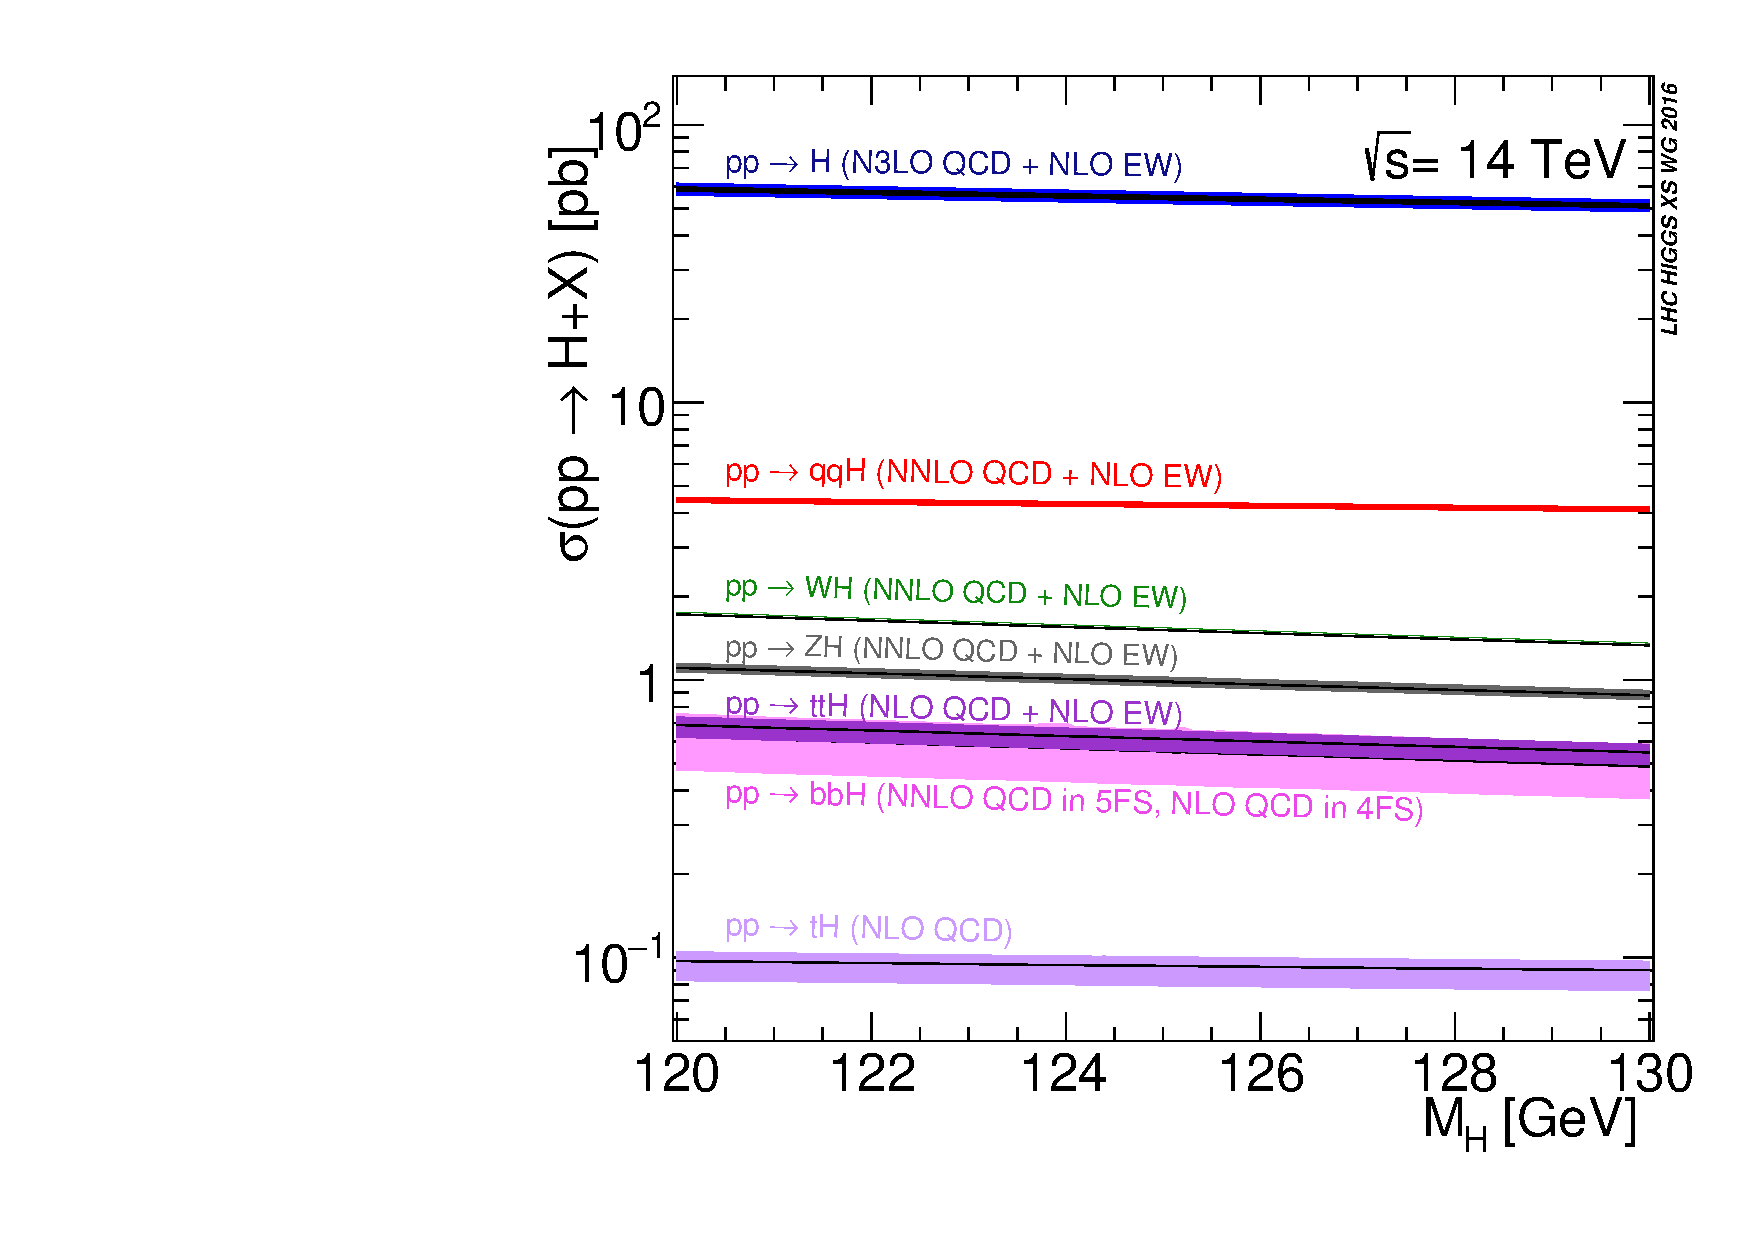
\includegraphics[scale=0.33]{H_cross_sections.pdf}}
\subfloat[][]{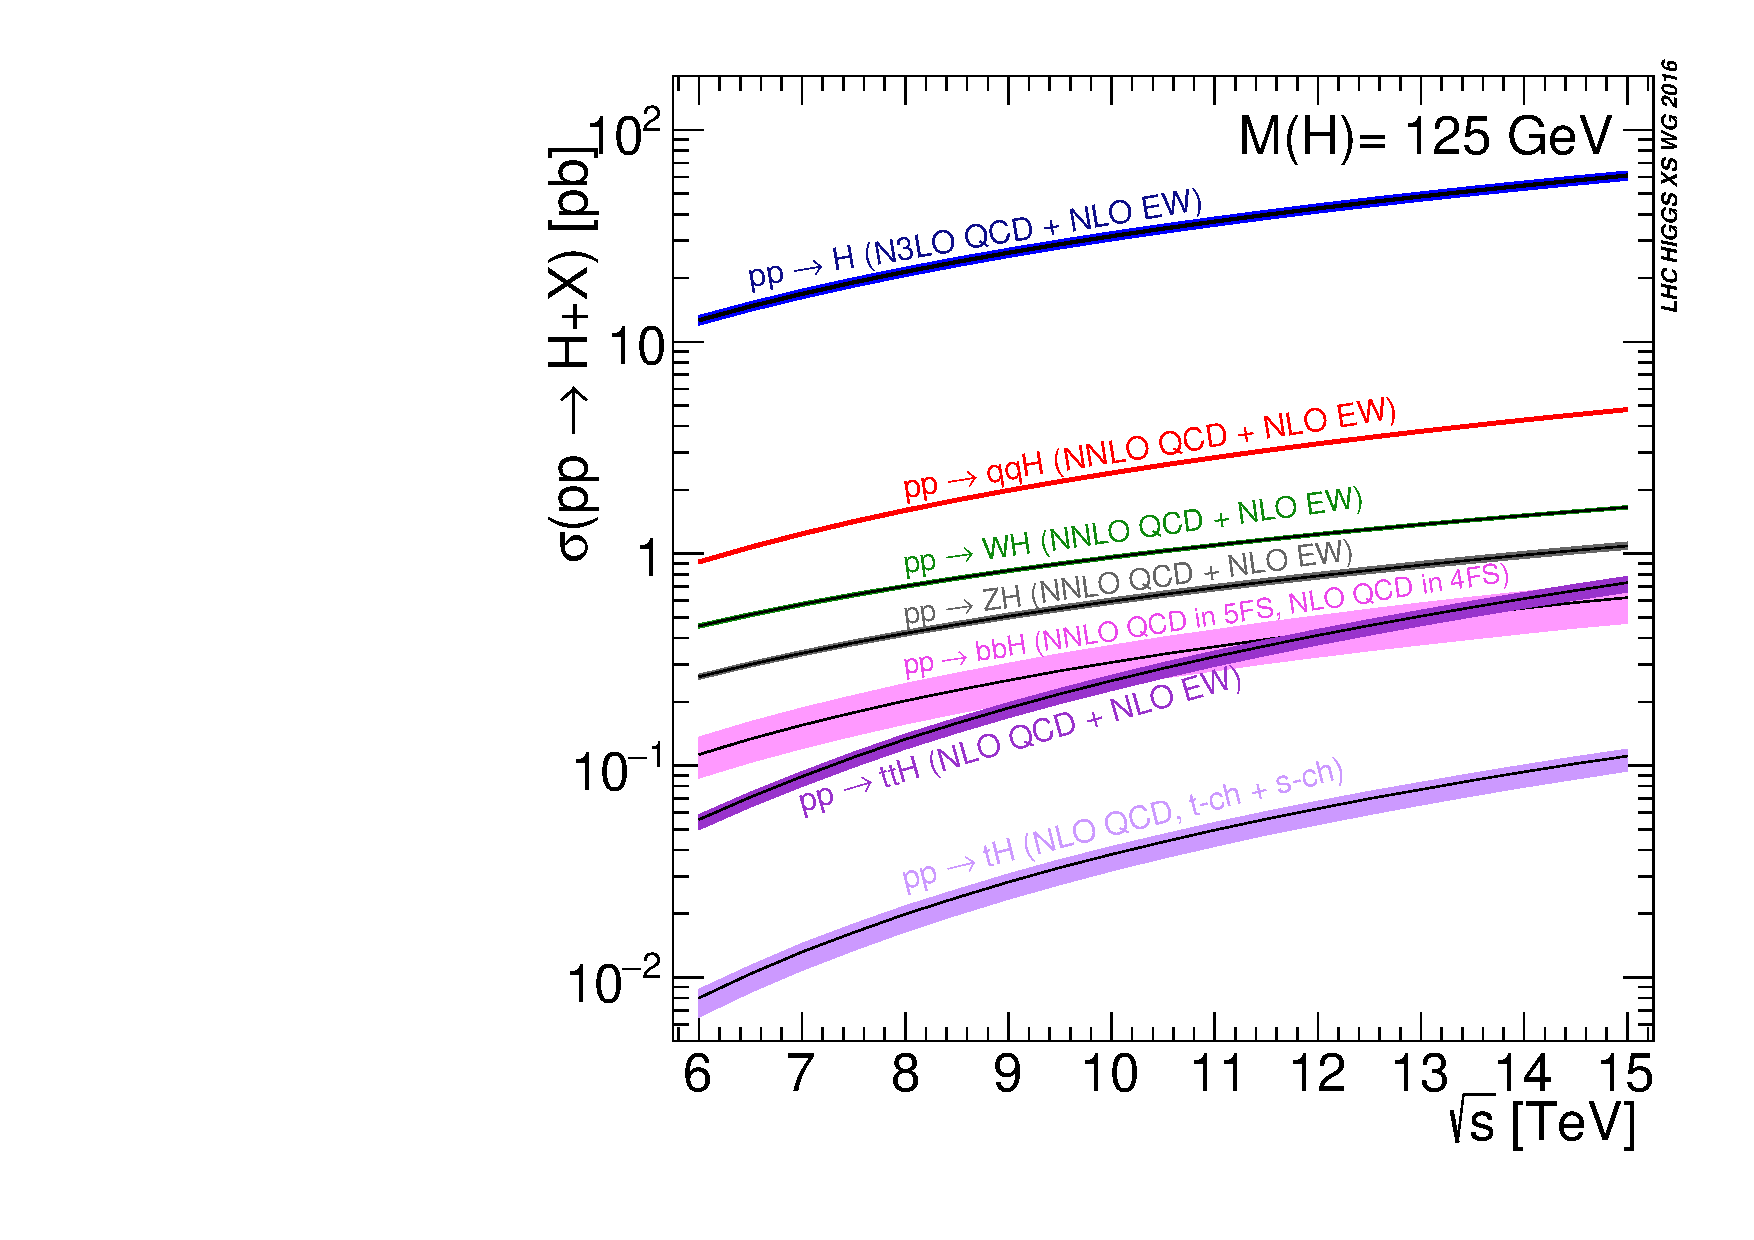
\includegraphics[scale=0.33]{cross_sec_energy.pdf}}
\caption{a)Higgs boson cross sections as a function of its mass for the various production modes, b)Higgs boson cross sections as a function of center-of-mass energy for the various production modes at $m_H = 125 \text{GeV}$.}
\label{H_cross_sections}
\end{figure}

\subsection{Higgs boson decay and the $\text{H} \rightarrow \gamma \gamma$ channel}
As any other Standard Model particle, the Higgs boson as well has a considerable manifold of processes concerning its decay channels. Each of these processes has a \emph{branching ratio} (BR), namely the fraction of decays that follows that process. These branching ratios are predicted by the Standard Model as a function of the Higgs mass (Figure \ref{H_BR}).
\\ \\
For very high masses, the leptonic decay channels mediated by W$^+$, W$^-$, or Z$^0$ bosons are the most probables for an Higgs event, while for masses up to around 130 GeV, the fermion-antifermion decay is the preferred decay mode and among the latter the $b\bar{b}$ stands out, because of its heavy mass and the consequent strong Higgs coupling.
\\
This large rate of $\text{gg} \rightarrow \text{H} \rightarrow \text{b}\bar{\text{b}}$ processes, on the other hand, has to compete with a very large background arising from the inclusive $\text{pp} \rightarrow \text{b}\bar{\text{b}} + \text{X}$due to the strong interaction.
\\
More simple to investigate becomes in this way the $\text{gg} \rightarrow \text{H} \rightarrow \gamma\gamma$ channel, where the Higgs boson decay into a pair of photons through a boson-loop or a fermion-loop, usually the W bosons are the most involved into the loop because of their strong coupling with the Higgs boson.
\begin{figure*}[h]
\centering
\subfloat{
	\feynmandiagram [small, horizontal=t1 to g1] {
  g1 --[boson] t1 -- [fermion] t2 --[fermion] t3 --[fermion] t1,
  g2 --[boson] t2,
  h -- [scalar, edge label = \small$H$]  t3,
  g1 --[opacity=0] g2,
};} \qquad
\subfloat{
	\feynmandiagram [small, horizontal=t1 to g1] {
  g1 --[boson] t1 -- [boson] t2 --[boson] t3 --[boson] t1,
  g2 --[boson] t2,
  h -- [scalar, edge label = \small$H$]  t3,
  g1 --[opacity=0] g2,
};}
\end{figure*}
\\The background for this channel derive from the processes with $\gamma\gamma$ and $\gamma$ + jet/dijet final states and can be splitted into two different categories: the reducible and the irreducible background. 
\\
\begin{itemize}
\item The reducible background is typically due to a $\pi^0$ decay from a main vertex of the hadronization jet. This kind of background it's quite easy to recognise, because the jet's deriving $\gamma$s not pass the photon isolation requirement for an Higgs event.
\item The irreducible background is composed of events where two photons are produced isolated, as well as for the signal. Typically the photons from these processes are produced directly in the main vertex and not in the jets, so they are isolated like the signal for the Higgs and it is not possible to distinguish between the two different kinds of events \cite{mass_measurement_ATLAS}.
\end{itemize}
\begin{figure}[htb]
\centering
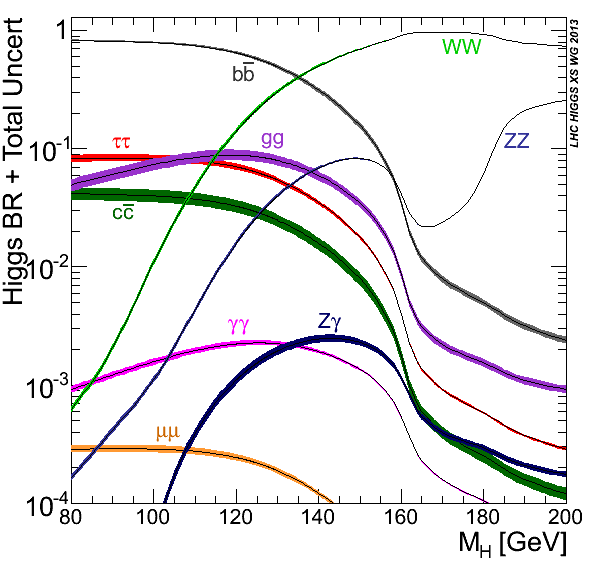
\includegraphics[scale=0.3]{H_BR.png}
\caption{Branching ratios for all of the Higgs decays, running over the whole mass spectrum.}
\label{H_BR}
\end{figure} 

\subsection{Experimental Higgs boson highlights}
Immediately after the discovery made by the ATLAS and CMS collaboration\cite{Observation_Higgs}, a considerable amount of measurements of the Higgs boson features has been performed, in order to establish the properties of the particle. Even if studies for such exotic beyond Standard Model Higgs bosons multiplets are still running, latest results from both the experiments involved in the research are consistent with Standard Model expectations for the Higgs boson.
\\\\
Starting from the mass measurement, achieved using Run1 results for $\text{H} \rightarrow \text{ZZ}^*$ and $\text{H} \rightarrow \gamma\gamma$ processes of both ATLAS and CMS experiments, which is found to be $m_H = 125.09 \pm 0.24 (\text{stat.}) \pm 0.11 (\text{syst.}) \text{GeV}$\cite{Aad2015zhl}, many other properties are still under investigation:
\begin{itemize}
\item the signal strength modifier $\mu$,
\item the couplings with fermions and bosons and their relative coupling-strength modifiers $k_j$,
\item the total decay width of the resonance of the particle
\end{itemize}
The signal strength $\mu_i$, which is the ratio between the observed production cross section $\sigma_i$ and the Standard Model's predicted value $\sigma_{SM}$ for a given mass hypothesis
\begin{equation}
\mu_i = \frac{\sigma_i}{\sigma_i^\text{SM}} \hspace{1cm} i \hspace{0.1cm} \text{: production modes}
\end{equation}
has been measured for each production mode separately.
\phantom{i}
\\
\phantom{i}
\begin{figure}[htb]
\centering
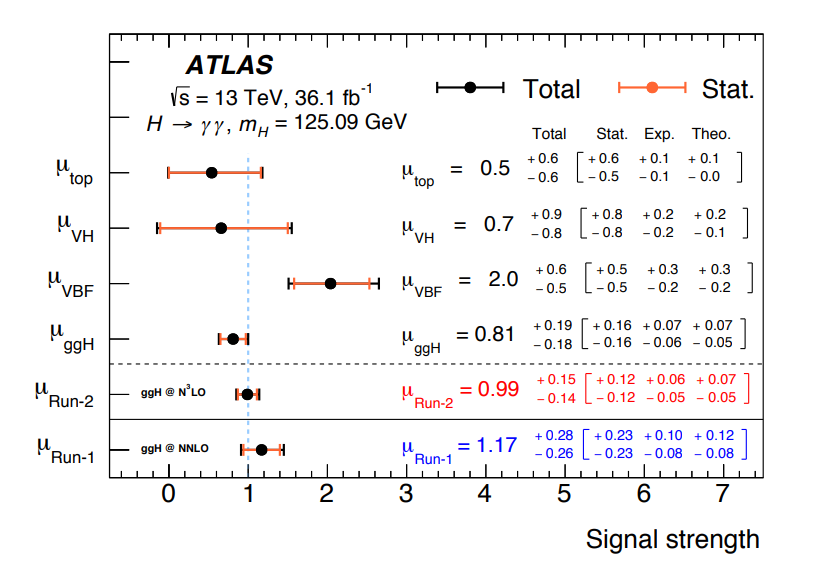
\includegraphics[scale=0.3]{signal_strength.png}
\caption{Signal strength's values measured for the different production modes (ggH, VBF, VH and top) and globally ($\mu_{Run2}$), compared with the global value ($\mu_{Run1}$).}
\end{figure}
\\The best-fit value for the signal strength, calculated for each production mode and corresponding to the measured mass of the particle, is found to be 
\begin{equation}
\mu_{ggH} = 0.81\hspace{0.06cm}^{+0.19}_{-0.18}\hspace{0.2cm} \text{,} \hspace{0.4cm} \mu_{VBf} = 2.0\hspace{0.06cm}^{+0.6}_{-0.5} \hspace{0.2cm} \text{,} \hspace{0.4cm} \mu_{VH} = 0.7\hspace{0.06cm}^{+0.9}_{-0.8} \hspace{0.2cm} \text{,} \hspace{0.4cm} \mu_{top} = 0.5\hspace{0.06cm}^{+0.6}_{-0.6} \hspace{0.4cm} \text{.}
\end{equation}
Then, the combination of all of the production modes brings to a value for the combined signal strength of
\begin{equation}
\mu_{comb} = 0.99\hspace{0.06cm}^{+0.15}_{-0.14}
\end{equation}
As well as the signal strength is the ratio between observed and predicted cross section, the coupling strength $k_i^2$ is the ratio between the observed coupling of the considered process $g_i$ and its predicted value for that process $g_i^{SM}$.
\begin{figure}[!b]
\centering
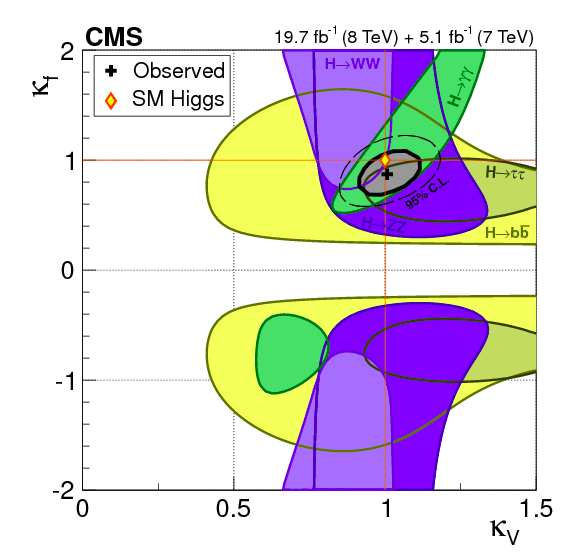
\includegraphics[scale=0.37]{kb_kv_Higgs.png}
\caption{Measurements of universal couplings for each production mode. The Model confirms the Standard Model prediction at 68\% CL.}
\end{figure}
\\In the k-framework, the cross section for an entire Higgs process is
\begin{equation}
\sigma(i \rightarrow H \rightarrow f) = \frac{\sigma_i(\vec{k}) \cdot \Gamma^f(\vec{k})}{\Gamma_H} \hspace{0.6cm}
\end{equation}
and all the possible deviations from the Standard Model predictions are described by the $k_j$ functions trough the relation
\begin{figure}[htb]
\centering
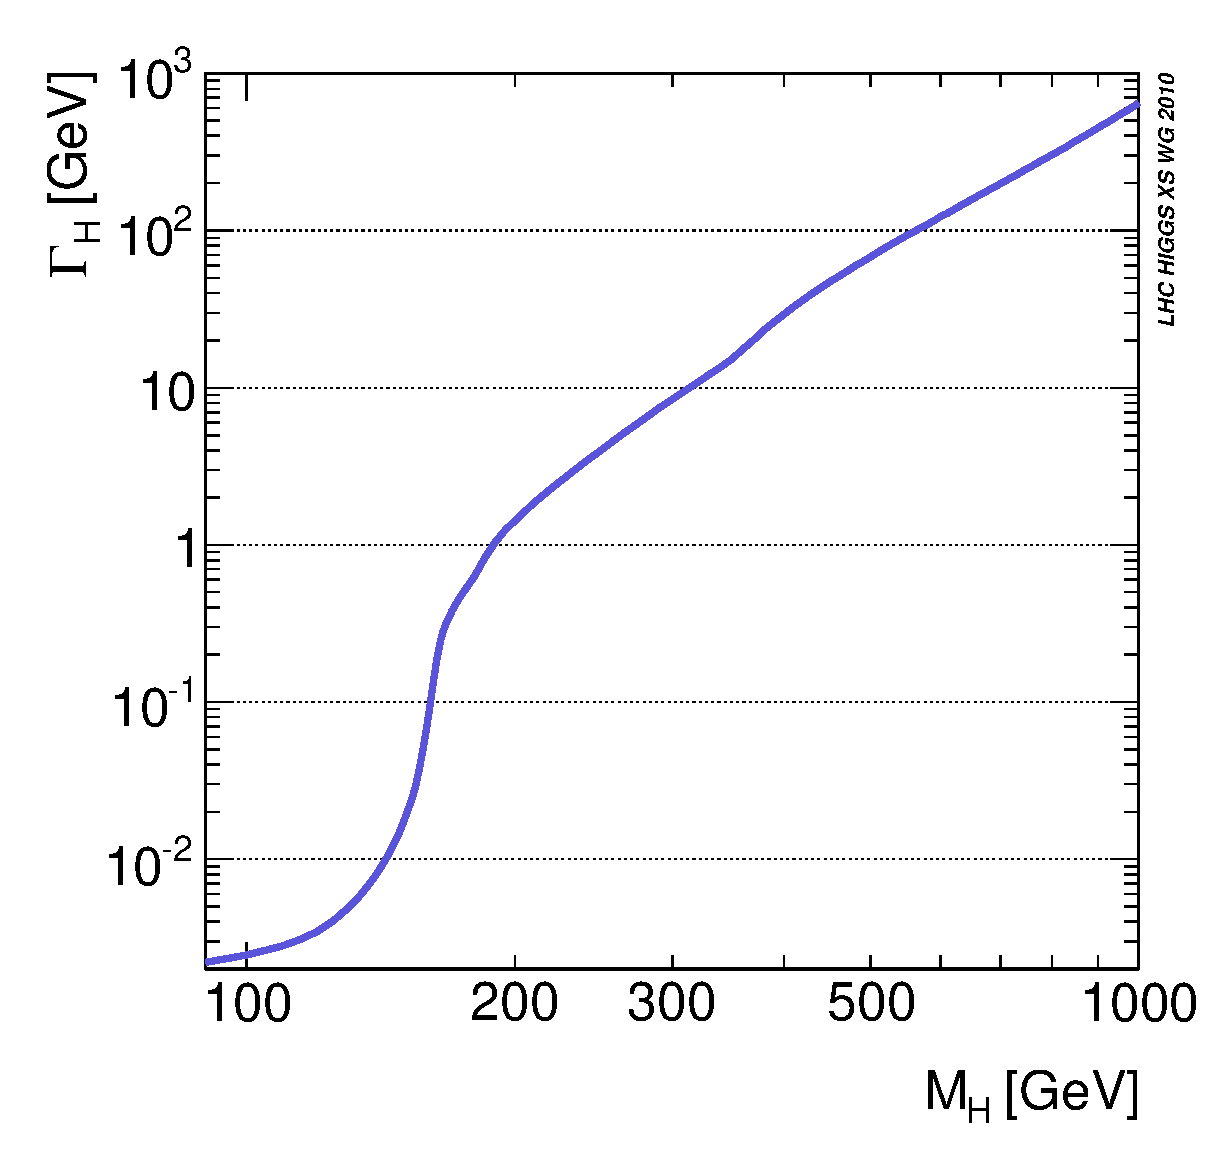
\includegraphics[scale=0.36]{total_decay_rate_Higgs.eps}
\caption{Total decay width for the Higgs boson predicted by Standard Model, as a function of it mass $m_H$.}
\label{total_decay_rate}
\end{figure}
\phantom{i}
\begin{equation}
\sigma_i = k_i^2(\vec{k}) \cdot \sigma_i^{\text{SM}} \hspace{0.4cm} \Longrightarrow \hspace{0.4cm} \Gamma^f = k_f^2(\vec{k}) \cdot \Gamma^{f, \text{SM}}
\end{equation}
Can be assured a universal coupling modifier $k_F$ for all fermions, and similarly a universal coupling modifier $k_V$ for all vector bosons.
\\
The total decay rate in the Standard Model is predicted as a function of the Higgs mass. In Figure \ref{total_decay_rate} you can see how, for masses of $m_H \simeq 125 \text{GeV}$, the total width is predicted by the Standard Model as a narrow resonance, with a total decay width of around 4.1 MeV. Combining results from different decays, the upper limit at 95\% CL on Higgs boson total decay width is calculated to be \cite{Khachatryan2016}
\begin{equation}
\Gamma_H^{\text{obs}} < 13 \text{MeV} \hspace{0.2cm} \text{.}
\end{equation}
\chapter{The Large Hadron Collider}
\label{capitolo_2}
The Large Hadron Collider (LHC) is the largest proton and heavy ions accelerator and collider ever built. It is designed to overcome the performances of the old kinds of accelerators, like Tevatron $\text{p}\bar{\text{p}}$ collider at Fermilab and the Lep $\text{e}^+\text{e}^-$ collider at Cern. The LHC was thought and designed to reach center-of-mass energies in order of 14 TeV with an instantaneous luminosity of $10^{34} \text{cm}^{-2}\text{s}^{-1}$ in proton-proton collisions. After some relevant technical issues which caused the reduction of the collisions energy in the early years since the switching on, at the state of art the accelerator works at its best performances.
\\\\
The idea of colliding proton instead of electrons is due to some physical constrains. Accelerating electrons in a circular path implies a huge amount of radiative energy losses. A charged particle in fact, if circularly accelerated, loses energy according to the relation\cite{jackson_classical_1999}
\begin{equation}
\frac{dE}{dt} \propto \frac{E^4}{m^4}
\end{equation}
where $E$ is the energy of the particle and $m$ is the mass. It is evident how the energy losses will be smaller for high masses and comparing the values for a proton and an electron, it turns up that in order to accelerate the latter to the same energy of a proton you have to compensate for an energy loss which is $(m_p / m_e) \sim 10^{13}$ higher.
\\\\
The draw back is that protons, unlike the electrons, are not elementary particles, but they are composed of partons and all of them will produce a lot of low-energy interactions, called \emph{underlying event}, that will interfere with the signal.

\section{The acceleration chain and LHC structure}
The LHC collider consists of a 27-kilometre ring of superconducting magnets and accelerates particles at energies up to the nominal value of 14 TeV in the center of mass through several stages \cite{Bruning}.
\\
For protons, the accelerator chain is composed of four stages, usefull to allow the particles rising the energy scale and focus the beams to increase the luminosity:
\begin{itemize}
\item a Linear Accelerator (LINAC) handles the very first part of the acceleration process, boosting the particles up to 50 MeV using Radio Frequency Quadrupoles (RFQ) and focusing quadrupole magnets;
\item the  Proton Synchrotron Booster, a circular accelerator consisting of four superimposed synchrotron rings, keeps on accelerating protons up to energies of 1.4 GeV;
\item the Proton Synchrotron (PS), a single synchrotron ring with a circumference of approximately 600 m, is where the protons reach an energy of 25 GeV;
\item the Super Proton Synchrotron (SPS), the upgraded model of the Proton Synchrotron with a  circumference of around 7 km, is the last link in the acceleration chain before the injection and speeds up the particles to 450 GeV.
\end{itemize} 
\begin{figure}[t]
\centering
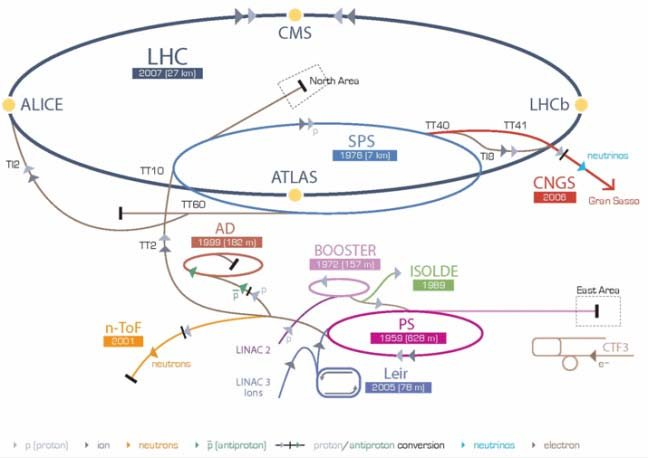
\includegraphics[scale=0.35]{CERN-accelerator-complex.jpg}
\caption{Accelerator complex at CERN}
\end{figure}
After the transition in the acceleration chain, protons are injected into LHC and they finally reach the nominal energy of $\sqrt{s}/2$. The beams travel in opposite directions in separate beam pipes, two ultra-high vacuum tubes, and are bended in the circular trajectory by a strong magnetic field mantained by superconducting deflecting dipole magnets, which operate at temperature of 1.9 K and produce a field of about 8.4 Tesla at a current of 11,700 A. The beam focusing relies on 392 quadrupole magnets acting on horizontal or vertical plane, depending on their polarity.
\\
The magnets are disposed along the ring in a modular layout, where each module is composed of six dipole magnets and two quadrupole magnets with opposite polarity. In order to fix the field non uniformities and so guarantee the stability of the two colliding beams, higher order magnets are installed at the end of the dipoles.
\\
At its full intensity, each proton beam is made of 2808 bunches of $10^{11}$ protons each and and collide with each other at four different interaction points where the main experiments are sited.
\vspace{0.3cm}
\begin{figure}[t]
\subfloat[][]{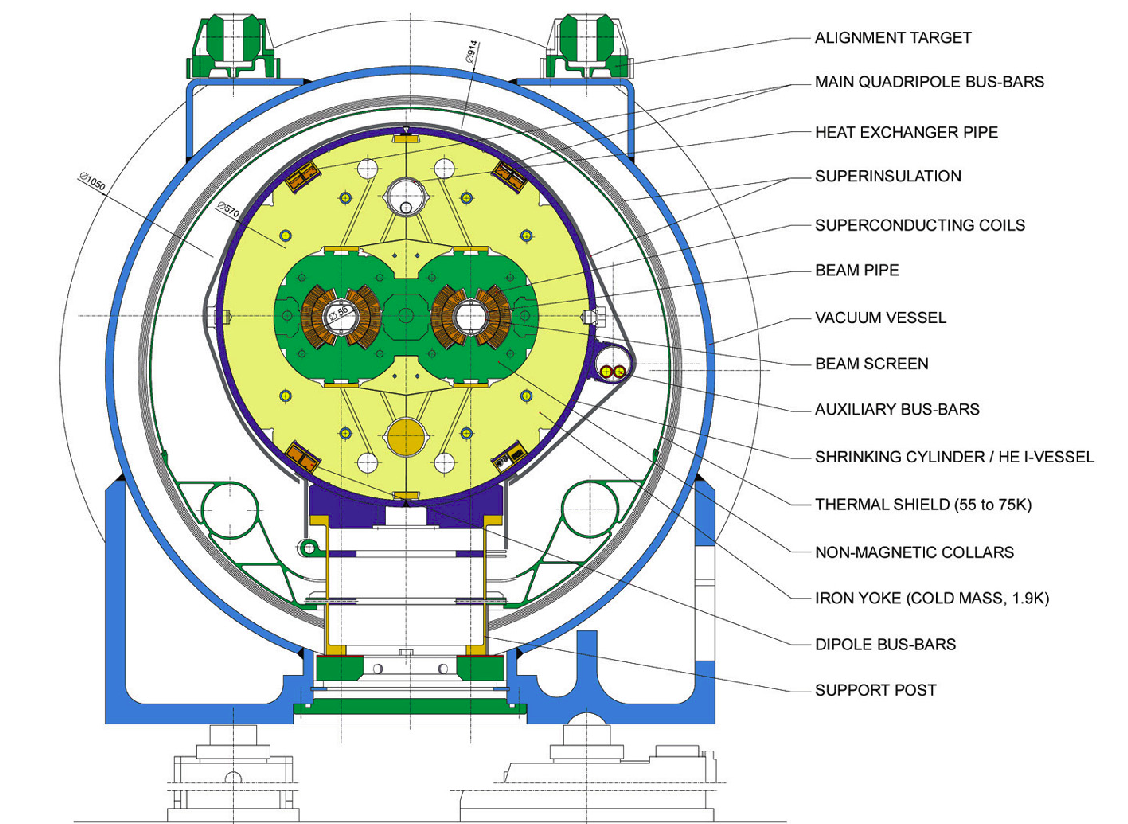
\includegraphics[scale=0.16]{dipole_magnet.png}}
\subfloat[][]{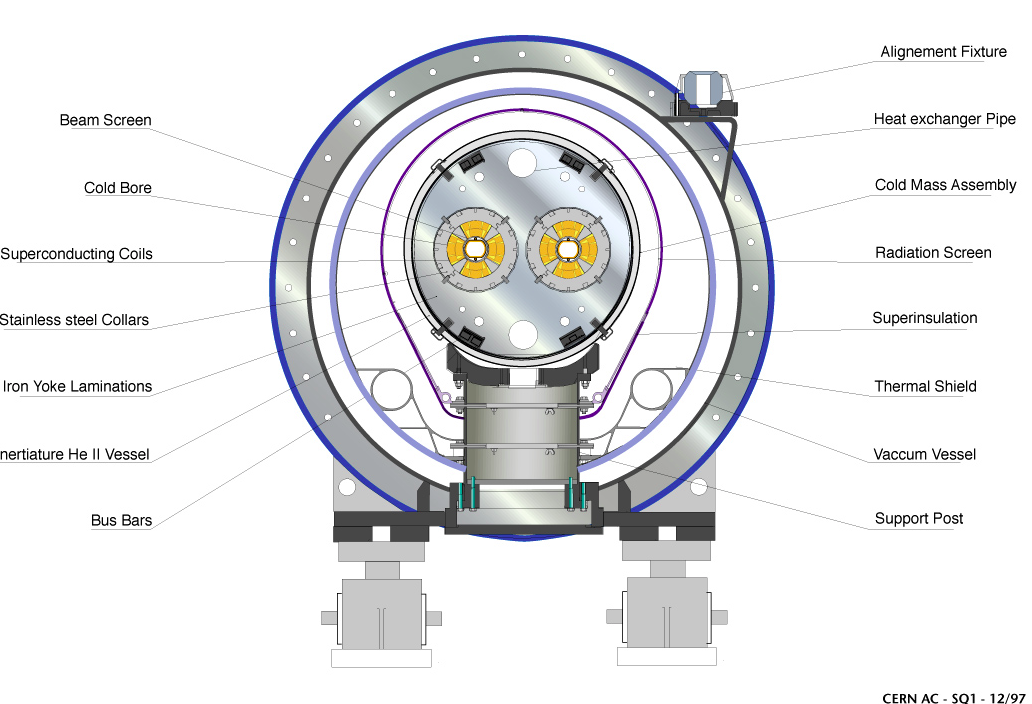
\includegraphics[scale=0.2]{quadrupole_magnet.png}}
\caption{a)Cross-section of the LHC dipole magnets, b)Cross-section of the LHC quadrupole magnets.}
\end{figure}
\\Checking the performaces of the collider, the main parameter to take into account is the instantaneous luminosity, which gives the rate of expected events of a process, once the cross section is known\footnote{The LHC nominal luminosity is $\mathcal{L} = 10^{34}\text{cm}^{-1}\text{s}^{-1}$, involving around one billion proton interactions per second.}
\begin{equation}
\frac{\text{d}N_{process}}{\text{d}t} = \mathcal{L}\sigma_{process}
\end{equation}
where $\sigma_{process}$ is the inelastic proton-proton cross section and
\begin{equation}
\mathcal{L} = f \frac{n_1n_2}{4\pi \sigma_x\sigma_y}
\end{equation}
where $f$ is the bunch crossing frequency, $n_1$ and $n_2$ are the numbers of particles in each bunch and $\sigma_x$ and $\sigma_y$ are the beam widths in the transverse plane.
Going more into LHC details, it can collide bunches of protons with a bunch crossing frequency of 40 MHz, each of them focused to reach down to 15 $\mu\text{m}$ in the transverse plane\cite{Bruning}. Integrating the instantaneous luminosity over a time period, you can find the integrated luminosity
\begin{equation}
L = \int\mathcal{L}dt
\end{equation}
\begin{table}[htb]
\caption{Design and 2016 LHC technical running conditions for proton-proton collisions \cite{LHC_parameters}.}
\centering 
\begin{tabular}{l l}
\hline\hline
\textbf{Parameters} & \textbf{Values} \\ [0.5ex]
\hline
Beam energy at LHC injection & 450 GeV \\
Design beam energy at collision & 7 TeV \\
2016 beam energy at collision & 6.5 TeV \\ [0.5ex]
\hline
Peak magnetic dipole field & 8.33 T \\
Dipole operating temperature & 1.9 K \\ [0.5ex]
\hline
Design instantaneous luminosity & $10^{34} \text{cm}^{-1}\text{s}^{-1}$ \\
2015-18 instantaneous luminosity & $1.2 \cdot 10^{34} \text{cm}^{-1}\text{s}^{-1}$ \\ [0.5ex]
\hline
No. of bunches per proton beam & 2808 \\
No. of proton per bunch (at start) & $1,15 \cdot 10^{11}$ \\
Bunch spacing & 25 ns \\
Minimum distance between bunches & $\sim 7 \text{m}$ \\ [0.5ex]
\hline
Beam lifetime & 10 h \\
Average collision rate & 36.1 MHz \\
Number of collision per second & 600 millions \\ [0.5ex]
\hline\hline
\end{tabular}
\end{table}
\\Tipically the luminosity is not constant during the data taking, but it is subject to decrease as the time goes on. This behaviour is due in particular to the degradation of the intensity of the beam, as a result of proton-proton collisions in the LHC interaction points.  Said that, the luminosity of the collider, seen as a function of time, is
\begin{equation}
\mathcal{L}(t) = \frac{\mathcal{L}_0}{(1+t/\tau_{nuclear})^2}
\end{equation}
with
\begin{equation}
\tau_{nuclear} = \frac{N_{tot,0}}{\mathcal{L}_0\sigma_{tot}k}
\end{equation}
\begin{figure}[htb]
\centering
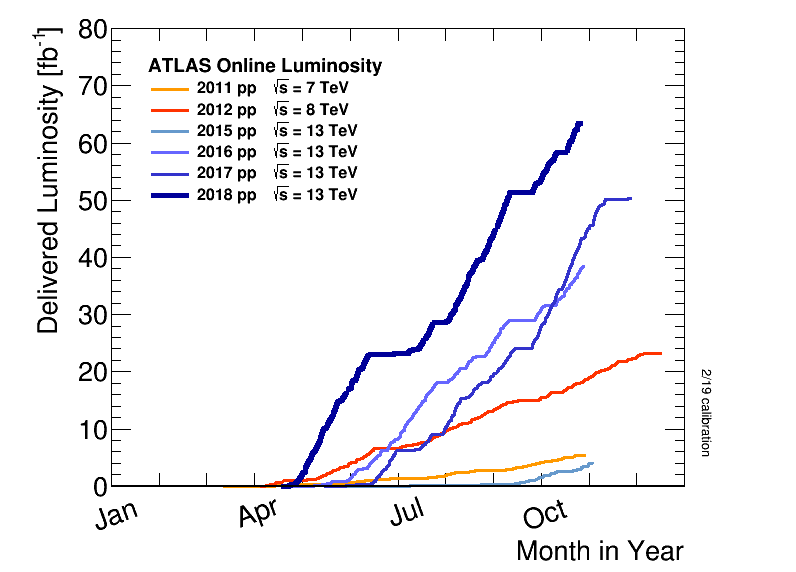
\includegraphics[scale=0.28]{luminosity.png}
\caption{Cumulative luminosity versus day delivered to ATLAS during stable beams and for high energy proton-proton collisions.}
\end{figure}
where $N_{tot,0}$ is the initial beam intensity, $\mathcal{L}_0$ is the initial luminosity at the beam injection $\sigma_{tot}$ stands for the total $pp$ cross section and $k$ is the number of interaction points\footnote{Around the main LHC ring, four different experiments are placed: ATLAS, CMS, LHCb and ALICE. The beams collide into each of these experiments, so at LHC four interaction points are present.}.
\\
In high-luminosity colliders, such as LHC, there is a considerable probability that a single bunch collision may produce several separate events, uncorrelated from the main interaction vertex and deriving usually from soft scattering processes: these kinds of event are known as \emph{pileup} events and are considered as background. The pileup events are strongly related to the instantaneous luminosity and affect the objects reconstruction, making the identification of vertices and tracks more difficult because of the increasing in the number of hits in each collision.
\\
The connection that tie the pileup events rate and the instantaneous luminosity is
\begin{equation}
\mathcal{L} = \frac{\text{rate}_{inelastic}}{\sigma_{inelastic}} = \frac{\mu n_b f_{rev}}{\sigma_{inelastic}}
\end{equation}
where $\mu$ is the number of inelastic interactions per bunch crossing and $n_b$ is the number of colliding bunches in the accelerator. The number of pileup events per bunch crossing is proportional to $\mathcal{L}/f$ and it increases with the instantaneous luminosity.
\begin{figure}[h]
\centering
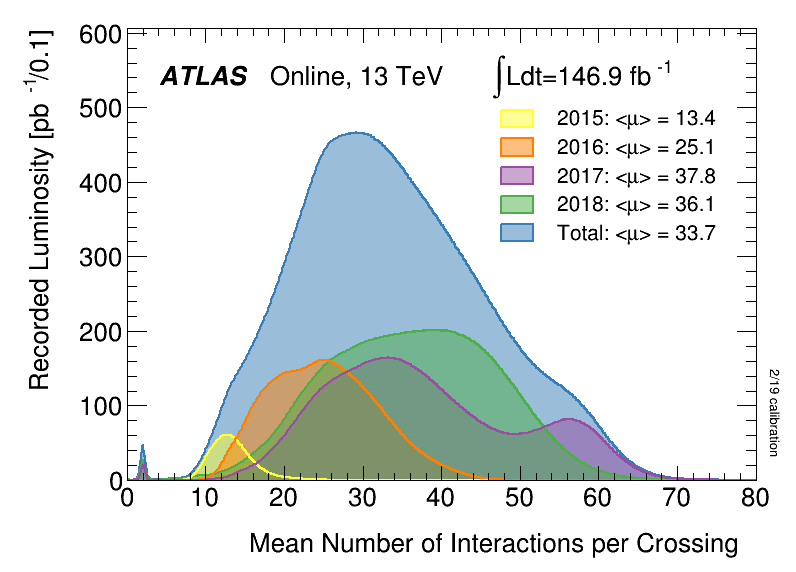
\includegraphics[scale=0.28]{pileup_events.png}
\caption{The luminosity-weighted distribution of the mean number of interactions per crossing for the 2018 pp collision data at 13 TeV centre-of-mass energy.}
\end{figure}


\section{Hadron colliders kinematics}
Because of the fact that hadron colliders run in the relativistic regime, the center-of-mass energy is generally boosted along the beam direction. To describe these kinds of events, a set on kinematic variables invariant under Lorentz boosts in that direction must be used.
A convenient set of these variables is the transverse momentum $p_T$, the  pseudo-rapidity $\eta$ or rapidity $y$ in the limit of a particle is travelling close to the speed of light and the azimuthal angle $\phi$. Using them to redefine the four-momentum $p^{\mu}$ of a particle of mass $m$, this can be written as
\begin{equation}
p^{\mu} = (E, p_x, p_y, p_z) = (m_T\cosh y, p_T\sin\phi, p_T\cos\phi, m_T\sinh y)
\end{equation}
where $p_x$, $p_y$ and $p_z$ are the spatial components of the momentum\footnote{In the third component $p_z$ of the momentum $\vec{p}$ of the particle is directed along the beam direction, while $p_x$ and $p_y$ lie in the transverse $(x,y)$ plane, perpendicular to the beam direction. The $x$ direction points toward the center of the LHC ring and the $y$ direction aims up from the $(z,x)$ plane.}
and the transverse mass $m_T$ is defined as $m_T = \sqrt{p_T^2 + m^2}$.
\\
The pseudo-rapidity $\eta$ describes the angle of a particle relative to the beam axis and it is defined as
\begin{equation}
\eta = -\ln\Bigl[\tan\Bigl(\frac{\theta}{2}\Bigr)\Bigr]
\end{equation}
where $\theta$ is the angle between the particle momentum $\vec{p}$ and the positive $z$ axis. Expressing $\eta$ in terms of the momentum $\vec{p}$, turns out to be
\begin{equation}
\eta = \frac{1}{2}\ln\Bigl(\frac{|\vec{p}| + p_L}{|\vec{p}| - p_L}\Bigr)
\end{equation}
where $p_L$ stands for the component of the momentum along the beam axis.
\\\\
In the limit of very high-energiy particles\footnote{In this limit, the particle's only energy is its momentum-energy, similar to the case of photons.}
, namely when the mass of the particle is negligible and so $m \ll |\vec{p}| \Rightarrow E \approx |\vec{p}|$, the pseudo-rapidity can be reasonably approximated with the definition of rapidity $y$
\begin{equation}
y = \frac{1}{2}\ln\Bigl(\frac{E + p_L}{E - p_L}\Bigr) \hspace{0.4cm} \text{.}
\end{equation}
Notice how the rapidity $y$ is not invariant under Lorent's boosts along the beam direction, but it transforms such as
\begin{equation}
y \longrightarrow y + \frac{1}{2}\ln\Bigl(\frac{1 + \beta}{1 - \beta}\Bigr)
\end{equation}
where $\beta$ is the boost velocity.
\\
Another common variable used to parametrise the angular separation between particles produced in an hadron collision is $\Delta R$, which is defined as
\begin{equation}
\Delta R = \sqrt{(\Delta\eta)^2 + (\Delta\phi)^2}
\end{equation}
where $\Delta\eta$ and $\Delta\phi$ are the differences in the $\eta$ and $\phi$ coordinates for the particles, respectively.
\chapter{The ATLAS detector at LHC}
\label{capitolo_3}
The ATLAS experiment\cite{Collaboration_2008} is one of the four major experiments at the Large Hadron Collider at CERN. It is, together with the CMS experiment, a general-purpose experiment, both designed to exploit the huge range of physics that the LHC provides.
\\\\
The cylindrical shaped detector is 46 m long and it has a radius of 12 m. It weights roughly 700 tons and sits in a cavern 100 m underground. The ATLAS detector is nominally forward-backward symmetric with respect to the interaction point and it is composed by four sub-systems, used to distinguish the particles arising from the interaction vertex, that radially from the closest to the outer one from the beam pipe are
\begin{itemize}
\item the Inner Detector (ID) is the very first step in the detection chain, located very close at the interaction point. It is designed for charged particles tracking and helpful in the interaction vertices' reconstruction;
\item the Electromagnetic Calorimeter (ECAL) is placed just after the ID and it is designed to detect electromagnetically interacting particles, such as electrons and photons. In this calorimeter these particles release all their energy and do not continue their run through the other sub-systems;
\item the Hadronic Calorimeter (HCAL) is the last and the biggest\footnote{Typically you need much more interacting material to stop an hadron with respect to an electron, due to the differences in their interaction showers.} 
calorimeter in the chain, designed to catch charged and neutral hadrons. After this sub-detector ideally only muons and neutrinos will pass;
\item the Muon Spectrometer (MS) is the last sub-detector and its role is to detect the muons, highly penetrating particles, arising from the interaction vertices\footnote{The only kind of particles left, neutrinoes, cannot be detected because they interact only weakly. Their presence in the process can be derived through the missing energy analysis for the selected event.}.
\end{itemize}
\begin{figure}[h]
\centering
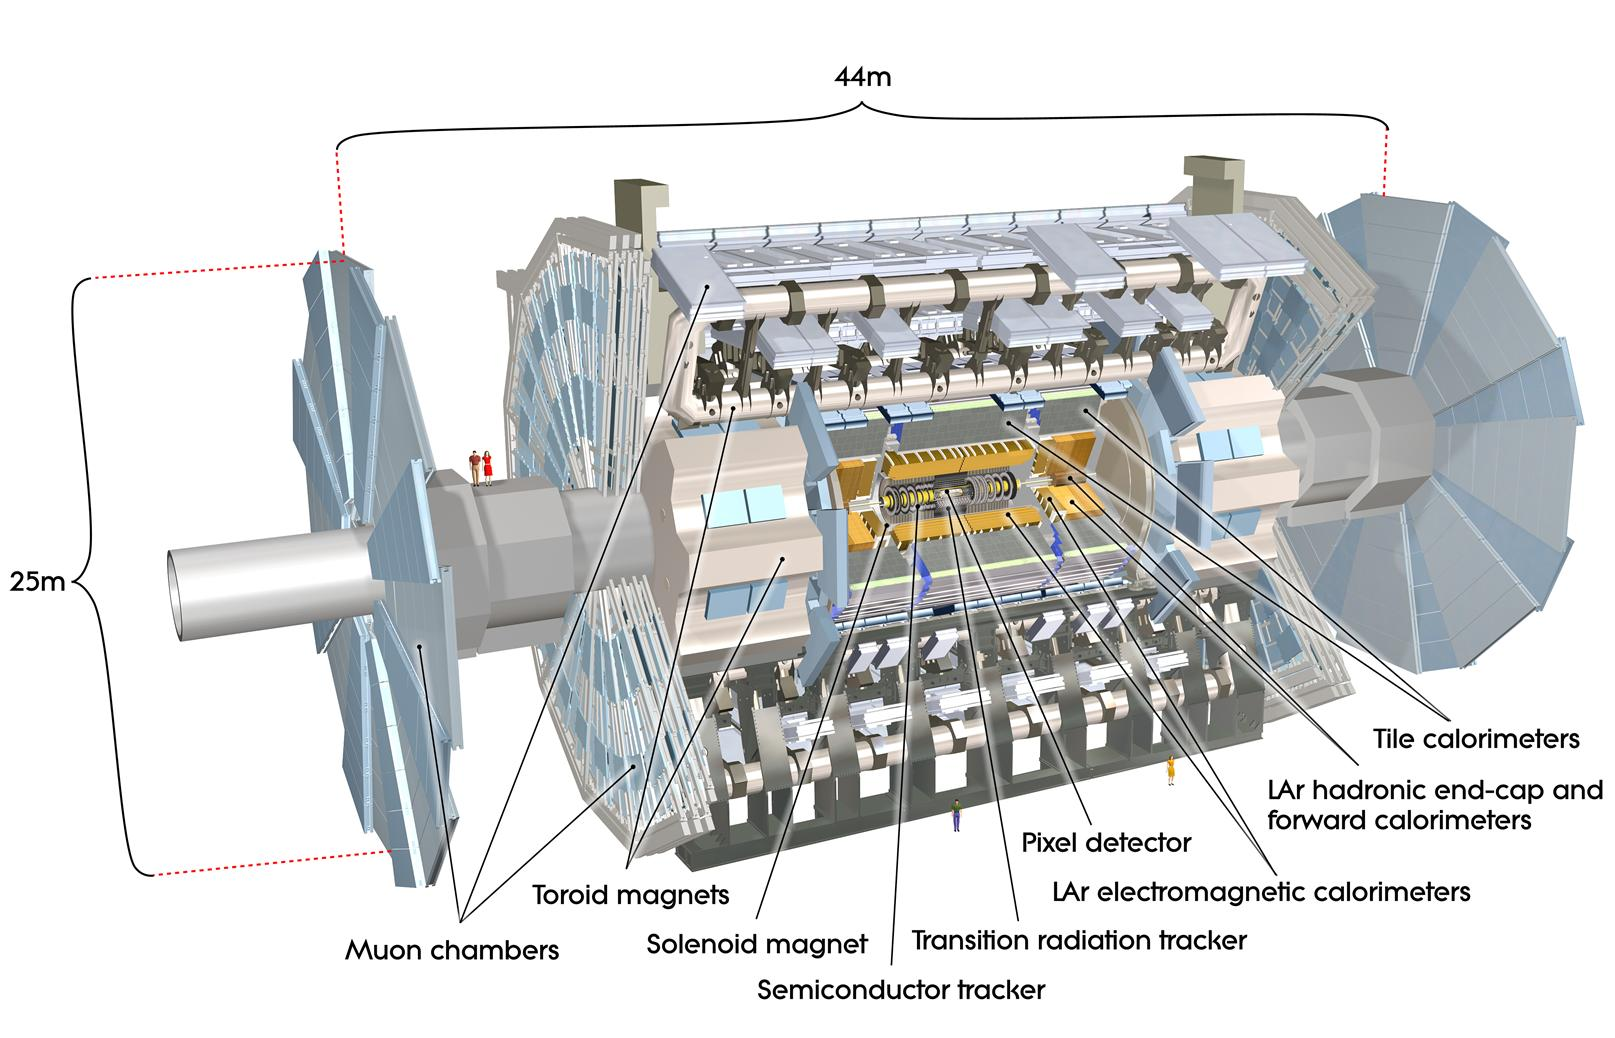
\includegraphics[scale=0.3]{ATLAS.jpg}
\caption{Cut-away view of the ATLAS detector.}
\end{figure}
The whole detector is covered by a magnet system that produces the electromagnetic field needed for measurement of the particles momenta.
\\
Integrated with the detector components there are the trigger and data acquisition system, a computing system which selects physics events with distinguishing characteristics and process them to extrapolate selected data.
\\
Being designed for general purposes, the detector must have a structure that allows to investigate a wide range of pyhsics, from the Higgs boson's analysis, to Standard Model measurements and future researches.

\section{The Inner Detector}
The ATLAS Inner Detector (ID)\cite{Aad:2010bx} is the first sub-detector which particles arising from the interaction find, just after the collision point. The detector is composed by a barrel and two end-cap regions to maximise the acquisition coverage, extending the pseudo-rapidity range up to $|\eta| < 2.5$ for particles coming from the LHC beam-interaction region, with full coverage in $\phi$. It is immersed in a 2 T magnetic field provided by a solenoid. Tracks measurements require a reasonably high resolution in the detection of the momentum of the particles and the multy-technology and high granularity of the Inner Detector increase the value of this parameter up to $\sigma_{p_T} / p_T = 0.05\%_{p_T} \text{GeV}$.
\\\\
Due to the extreme proximity at the interaction point, the ID design requires a high radiation resistance for all of its components and it is designed to detect particles using a series of different layers, as it can be seen in the split-view of Figure \ref{split-view}.
\\\\
\phantom{1}\hspace{0.3cm}The \emph{Pixel Detector} is the first sub-detector crossed by the particles produced in the interaction event. It is the real core in track reconstructing, because of its extremely high spatial resolution performance. The Pixel Detector consists of 1744 silicon pixel modules\cite{Aad_2008} arranged in three concentric barrel layers, positioned at radial dinstances of 50.5, 88.5 and 122.5 mm from the beam pipe, and two end-caps of three disks each, arranged at radial distances of 49.5, 58.0 and 65.0 mm respectively. The single module covers an active area of 16.4 mm $\times$ 60.8 mm and containts 47 232 pixels, most of size 50 $\mu$m $\times$ 400 $\mu$m.
\vspace{0.5cm}
\begin{figure}[t]
\centering
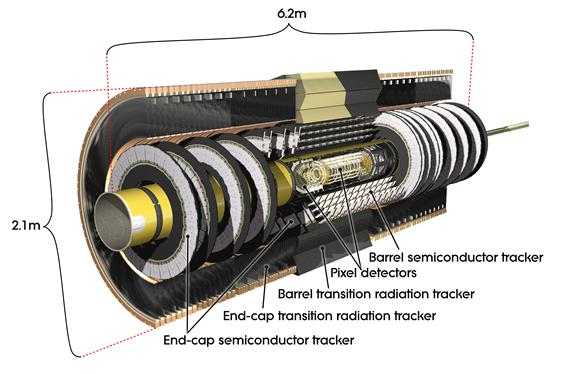
\includegraphics[scale=0.42]{inner_detector.jpg}
\caption{Split-view of the ATLAS Inner Detector}
\label{split_view}
\end{figure}
\\A module is read out by 16 radiation-hard front-end chips\cite{PERIC2006178} bonded to each sensor, so the total number of readout channels are $\sim$ 80.4 million. Hits in a pixel are read out if the signal exceeds a tunable threshold. Each particle crossing event defines tipically three measurement points for particles originating in the beam-interaction region.
\\
Between LHC Run1 and Run2 a fourth layer, konw as Insertiable B-Layer (IBL)\cite{Capeansjnh} has been installed between a new smaller beam pipe\footnote{The beam pipe diameter has been downcreased from 59 mm to 47 mm.} and the innermost layer (B-Layer) of the original Pixel Detector. This insertion in the tracking apparatus, so close to the interaction point, allowed to improve the quality of impact parameter reconstruction for tracks and thereby improving vertexing and $b$ tagging performance.
\\\\
\phantom{1}\hspace{0.3cm}The \emph{SemiConductor Tracker} (SCT) \cite{ABDESSELAM2006642, ABDESSELAM2007353} stands at the second stage of the particle tracking process, started with the Pixel Detector. It consists of 4088 modules of silicon-strip detectors arranged in four concentric barrels and two end-caps of nine disks each. In this way, as well as for the Inner Detector, the SemiConductor Tracker provides four more space points, placed at around 30, 37, 44 and 51 cm from the interaction point, bringing to eight the total number of space points for each particle's track. The intrinsic hit resolution of the SemiConductor Detector is a bit lower than for the Pixel Detector and it gets to $\sim 16 \mu$m along R-$\phi$ plane and $\sim 580 \mu$m along the z axis.
\\
Most modules consist of four silicon-strip sensors\cite{AHMAD200798} where two sensors on each side are chained together to give 768 strips of approximately 12 cm in length. A second pair of identical sensors is glued back-to-back with the first pair at a stereoangle of 40 mrad to provide space points. Since the detector is designed to perform tracking measurements, the hit informations gotten from an event is binary: once a particle hits the sub-detector, that will be registered only if the pulse height in a channel exceeds a preset threshold, normallycorresponding to a charge of 1 fC.
\\\\
\phantom{1}\hspace{0.3cm}The \emph{Transition Radiation Tracker} (TRT)\cite{collaboration_2008_TRT_barrel, collaboration_2008_TRT_endcaps} is the outer part of the tracking apparatus and covers radial distances from 563 mm to 1066 mm from the interaction point. It provides up to 36 additional space points to reconstruct the particles tracks, but the other side of the coin is its worst intrinsic spatial resolution of $\sim 130 \mu$m in the r-$\phi$ plane. The Transition Radiation Tracker is made of 298 304 proportional drift tubes, usually known as straws, with 4 mm in diameter, read out by 350 848 channels of electronics.The straws in the barrel region are arranged in three cylindrical layers and 32 $\phi$ sectors, while the straws in the endcap regions are radially oriented and arranged in 80 wheel-like modular structures.
\begin{figure}[h]
\centering
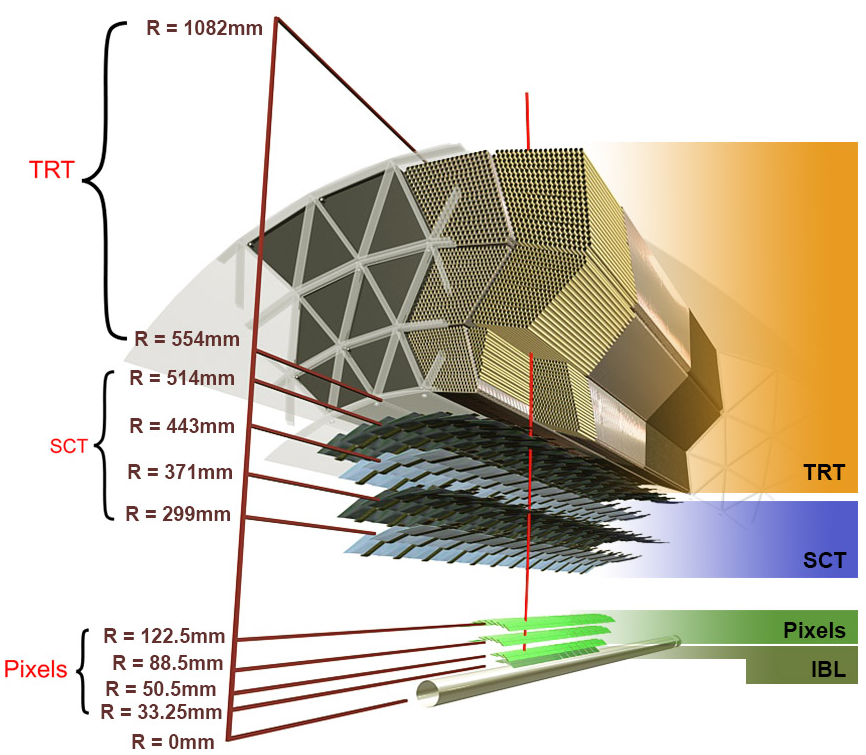
\includegraphics[scale=0.8]{split_view_ID.png}
\caption{Schematic view of the Inner Detector (ID) detailed layout, including the new Insertable B-Layer (IBL).}
\end{figure}
\\This kind of sub-detector works both as drift chamber measuring the charge drift time and as transition radiation detector to identify electrons by means of polypropylene fibres for the barrel or foils for the endcaps interleaved between the straws. The design of TRT allows charged particles with transverse momentum $pT>0.5$ GeV and with pseudo-rapidity of $|\eta| < 2.0$ to cross typically more than 30 straws.
\\\phantom{1}\hspace{0.3cm}The \emph{Cooling System} is designed to span a very wide range of temperatures, due to the peculiar operating environment for each sub-detector of the Inner Detector. The silicon detectors are cooled with a bi-phase evaporative system using C$_3$F$_8$ fluid at -25 \textdegree{}C. The target temperature for the silicon sensors is 0 \textdegree{}C for the Pixel Detector and -7 \textdegree{}C per the SemiConductor Tracker. These values were chosen to break down the radiation damages to the electronic systems.
\\\\
The overall Inner Detector relative momentum resolution before the IBL insertion 
\begin{equation}
\sigma_p / p = (4.83 \pm 0.16) \times 10^{-4}\text{GeV}^{-1} \times p_T
\end{equation}
has been measured for high momentum tracks.
\\
Since the amount of material to achieve the high granularity set in the Inner Detector, including read-out, cooling systems and supports, is quite sizable, some of the photons arising from the collision event may convert into electron-positron pairs before reaching the Electromagnetic Calorimeter as well as electrons may loose part of their energy through bremsstrahlung emissions. These kind of losses generally affect the energy resolution of the calorimeter system.

\section{The ATLAS calorimeters}
The ATLAS calorimeters system consists of three different types of sampling calorimeters, each of them designed to detect a precise family of particles. Typically the detection of photons and light particle electromagnetically interacting, such as electrons, is left to the Electromagnetic Calorimeter (ECal), covering the pseudorapidity region $|\eta| < 3.2$, while for hadrons the Hadronic Calorimeter (HCal) is preferred, with a pseudorapidity region of $|\eta| < 3.9$. To seal the system and to maximise the detection region, two Forward Calorimeters are sited at either end of the main barrel, to cover the pseudorapidity range of $3.1 < |\eta| < 4.9$ .
\\
The Calorimetric system have the main purpose of detecting particles by measuring the energy and the direction of incoming electrons, photons and hadrons, giving a fundamental contribution in the missing transverse energy measurement too.
\\
It consists of Sampling Calorimeters, where the absorbing material which degrades the energy of the particles and the active material that provides a measurable signal are alternated within the detector's volume. For ATLAS experiment calorimeters, Liquid Argon (LAr) or polystirene scintillator are used as active material, while lead (Pb), copper or iron are used as passive material.
\\
Passing through these layers, particles interact with the material producing showers whose energy and trajectory are measured. Depending on the nature of the incoming particle, it may start an electromagnetic shower, mainly detected in the electromagnetic calorimeter, or an hadronic shower, visible in the hadronic calorimeter.
\begin{figure}[h]
\centering
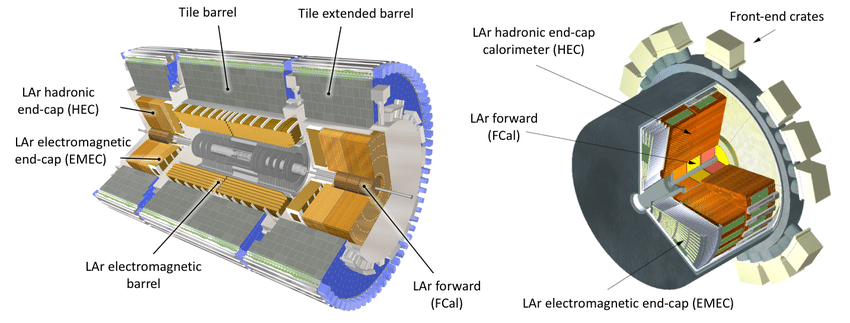
\includegraphics[scale=0.43]{calorimeters.png}
\caption{Subsystems of the ATLAS calorimeters and an enlarged view of the end-cap calorimeters.}
\end{figure}
\subsection{Electromagnetic showers}
At high energy, photons in matter convert into an electron-positron pair which then emit energetic bremsstrahlung photons. These, in turn, convert into further electron-positron pairs and so on. This chain reaction continue until the energy of the pair-produced electrons and positrons drops below an energy threshold, known as the \emph{critical energy} ($E_c$). Once that point is reached, the $e^+ e^-$ pairs will prefer atomic collisions rather than bremsstrahlung emission as energy loosing choice and breaking the cascade\cite{Leo302344}.
\\
The longitudinal development of the shower is governed by the \emph{Radiation Length} ($X_0$), defined as the amount of material which causes the electron to reduce its energy by a factor of $e$ \footnote{For Liquid Argon (LAr) and Lead (Pb), the critical energy and radiation length are
\begin{align*}
E_c^{LAr} = 32.84 \text{MeV} \hspace{0.2cm},& \hspace{0.4cm} X_0^{LAr} = 14 \text{cm} \\
E_c^{Pb} = 7.43 \text{MeV} \hspace{0.2cm},& \hspace{0.4cm} X_0^{Pb} = 0.56 \text{cm}
\end{align*}
Considering now an electron with an initial energy of $E_0 = 100 \text{GeV}$, the shower depth in LAr and Pb will be
\begin{align*}
L^{LAr}(95\%) &\sim 260 \text{cm} \\
L^{Pb}(95\%) &\sim 15 \text{cm}
\end{align*}}.
Considering $X_0$ related to the typical path necessary for a photon to create an $e^+e^-$ pair, the total number of particles in the shower after $t$ times $X_0$ turns out to be
\begin{equation}
N(t) = 2^t
\end{equation}
with an approximate energy for the single particle of
\begin{equation}
E(t)/\text{particle} = E_0/2^t
\end{equation}
Once the critical energy $E_c$ is reached, the shower stops and the maximum number of expected particles in the cascade can be calculated as
\begin{equation}
N_{max} \sim E_0 / E_c \hspace{0.2cm} \text{.}
\end{equation}
All of these parameters strictly depend on the atomic number Z of the detector material: in high-Z materials, particle multiplication continues longer and decreases more slowly than in low-Z materials or number of positrons strongly increases with the Z value of the absorber material.
\\
The critical energy $E_c$ is parametrized for liquid and solid materials as:
\begin{equation}
E_c = \frac{610 \text{MeV}}{Z+1.24}
\end{equation} 
where Z is the atomic number of the material, while the \emph{radiation length} ($X_0$) is definded as
\begin{equation}
X_0 = \frac{716.4[\text{g}\hspace{0.05cm}\text{cm}^{-2}] \times A}{Z(z+1)\ln(287/\sqrt{Z})} \hspace{0.2cm} \text{.}
\end{equation}
The material thickness needed to contain the 95 \% of the longitudinal energy profile of the shower is the \emph{shower depth}
\begin{equation}
L(95\%) \sim t_{max} + 0.08Z + 9.6 = \Bigl[\ln\Bigl(\frac{E_0}{E_c}\Bigr) + C_j \Bigr] + 0.08Z + 9.6 \hspace{0.5cm} [X_0]
\end{equation}
where $E_0$ is the energy of the incoming particle and $C_j$ is a parameter which can be $-0.5$ or $+0.5$ depending on the incident particle being an electron or a photon respectively. It is expressed in units of $X_0$.
\\\\
The last important parameter for electron and photon shower is the \emph{Moliere radius} ($R_M$), which is related to the lateral development of the shower and it is defined as
\begin{equation}
R_M = \frac{21 \text{MeV}}{E_c}X_0 \hspace{0.2cm} \text{.}
\end{equation}
Up to 95\% of an electromagnetic shower is enclosed in twice the $R_M$.

\subsection{Hadronic showers}
Considerably different from electrons and photons with electromagnetic showers, hadrons produce a shower of secondary particles, known as hadronic showers, within which two different kinds of processes are involved.
\begin{itemize}
\item The electromagnetic component represent up to 30-60\% of the total energy and it derives from $\pi^0$ pions decays into two collimated photons.
\item The hadronic component leads the main contribution at the shower generation combining several processes, such as slow neutrons production or spallation protons. Part of the energy released in the hadronic calorimeter does not contribute to the signal. This kind of invisible energy is due to the nucleons released in the nuclear reactions and represents up to 40\% of the total amount of energy liberated.
\end{itemize}
The main parameter which describes the hadronic showers is the \emph{nuclear interaction length} $\lambda_{int}$, representing the average distance a high-energy hadron has to travel inside a medium before a nuclear interaction occurs, is described as
\begin{equation}
\lambda_{int} \sim 35 A^{1/3} \text{g cm}^{-2} \hspace{0.2cm} \text{.}
\end{equation}
Similarly to the shower depth for electromagnetic showers, 95\% of the longitudinal energy deposit profile of the hadronic shower is contained in
\begin{equation}
t_{95\%} = t_{max} + 2\lambda E^{0.13}
\end{equation}
where $t_{max}$ is
\begin{equation}
t_{max} = 0.2\ln(E/1 \text{GeV}) + 0.7 \hspace{0.5cm} [\lambda]
\end{equation}
expressed in units of nuclear interaction length\footnote{Considering Liquid Argon (LAr) and Lead (Pb) and an incoming pion with $E_{\pi} = 100 \text{GeV}$, the values for $\lambda_{int}$ and $t_{95\%}$ are
\begin{align*}
\lambda_{LAr} = 85.77 \text{cm} \hspace{0.2cm} &, \hspace{0.4cm} t_{95\%}^{LAr} = 450 \text{cm} \\
\lambda_{LAr} = 85.77 \text{cm} \hspace{0.2cm} &, \hspace{0.4cm} t_{95\%}^{LAr} = 450 \text{cm} \hspace{0.2cm} \text{.}
\end{align*}}.
\\
Since $\lambda$ is much larger than the radiation length $X_0$, a considerable thicker detector\footnote{To contain a 100 GeV pion, a layer of Lead almost 6 times thicker than the one requested to contain a same-energy electron is needed.}. Therefore, in the experiment design usually electromagnetic calorimeters fit before the hadronic calorimeters.

\subsection{The ATLAS Electromagnetic Calorimeter}
The ATLAS Electromagnetic Calorimeter (ECal)\cite{CERN-LHCC-96-041, Aad2010ai} is composed of a central barrel region, which covers $|\eta| < 1.4$, and two end-caps to extend the $\eta$ region to $1.4 < |\eta| < 3.2$. It is a sampling calorimeter consisting of two half-barrels, centered around the ATLAS beam axis (typically the $z$-axis), where one of these half-barrels covers $z > 0$ and pseudorapidity $\eta > 0$ and the other covers $z < 0$ and pseudorapidity $\eta < 0$. The calorimeter itself is made of several 2 mm layers of Liquid Argon as active medium spaced out by Lead absorber plates with different thickness for $|\eta| < 0.8$ and $|\eta| > 0.8$\footnote{The Lead absorber plates have a thickness of 1.5 mm for $|\eta| < 0.8$, while 1.3 mm for $|\eta| > 0.8$.}
, glued between two 0.2 mm thick stainless steel sheet, in order to improve their mechanical strength. For ease of construction, both half-barrels are divided into 16 modules, each with a thickness of at least 22 radiation lengths ($X_0$), increasing from 22$X_0$ to 30$X_0$ between $|\eta| = 0$ and $|\eta| = 0.8$, and from 24$X_0$ to $33X_0$ between $|\eta = 0.8$ and $|\eta = 1.3$.
\\
Once assembled, active materials and absorbers are arranged into an accoridon-shape structure, leaving no discontinuity along the azimuthal angle $\phi$ and avoiding cracks due to the outgoing read-out system.
\\\\
The 275 $\mu$m read-out electrodes consist of three conductiove copper layers separated by insulating polymide sheets. The two outer layers are at the high voltage potential, while the inner one is used for reading out the signal through capacitive coupling.
\begin{figure}[h]
\centering
\subfloat{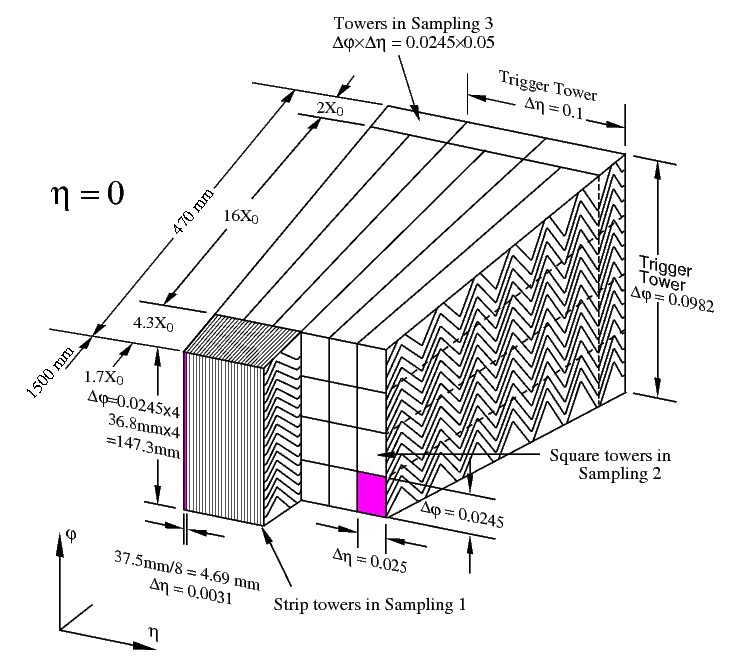
\includegraphics[scale=0.25]{calorimeter_sketch.png}}
\subfloat{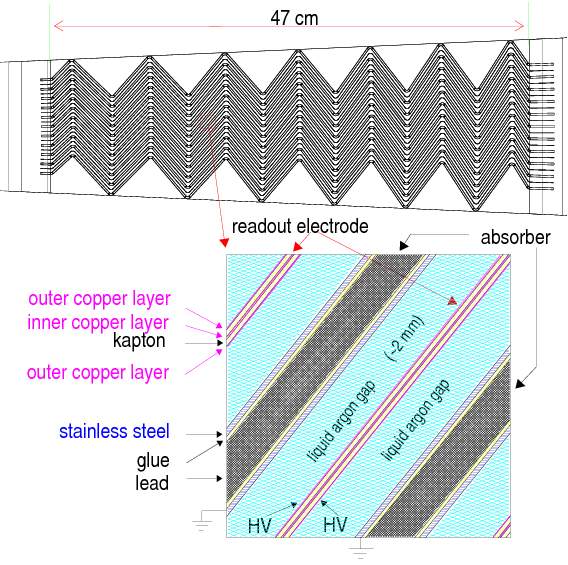
\includegraphics[scale=0.3]{accordion_structure.png}}
\caption{Sketch of a LAr calorimeter barrel module with a focus on the accordion structure and its layers granularity in $\eta$ and $\phi$.}
\end{figure}
\phantom{i}
\\To improve the precision in the recording of the longitudinal development of the electromagnetic showers, the Electromagnetic Calorimeter is segmented into four different longitudinal layers:
\begin{itemize}
\item The \emph{Presampler} (PS) is the innermost and thinnest layer of the system, with a thickness of 1.1 cm only and it is placed inside the solenoid, covering the $|\eta| < 1.8$ region. It is a single layer of Liquid Argon, but with no Lead absorber in front and it has been designed to correct for the energy loss in the Inner Detector, solenoid and cryostat wall;
\item The \emph{Layer 1} (L1) has a depth of 6 radiation lengths, including the material in front. This layer has the finest segmentation along $\eta$ with each strip of size $(\Delta \eta \times \Delta \phi) = (0.0031 \times 0.1)$, providing an excellent resolution in the $\eta$ coordinate in order to discriminate between photons related with the selected event and  $\pi^0$ decaying in two collinear photons;
\item The \emph{Layer 2} (L2) is where most of the energy is deposited and it extends the depth up to 22 radiation lengths. Clusters with energy below 50 GeV are generally fully contained in the Layer 2\footnote{Typically, the majoirty of the energy for showers generated by electrons or photons with energy up to 50 GeV is released in the 16 radiation lengths region.}. For the position measurement of the cluster, in this layer both $\eta$- and $\phi$-coordinates are equally important and therefore it is segmented into square cells of size $(\Delta \eta \times \Delta \phi) = (0.025 \times 0.025)$;
\item The \emph{Layer 3} (L3) completes the calorimeter layers, adding two more radiation lengths in the apparatus. Only the highest-energy electrons and photons can reach this deep in the detector in wide showers by now. For this reason the cell size in this layer can be doubled in the $\eta$ direction without loss of resolution. It is used to estimate the energy losses in the Hadronic Calorimeter placed right after.
\end{itemize}
In the end-cap there is less material in front of the calorimeter and the presampler can be avoided for $|\eta| > 1.81$. The end-caps start at $|\eta| = 1.5$ and continue down to $|\eta| = 3.2$ but with an increased cell size above $|\eta| = 2.5$ . The most critical point in the calorimetric apparatus is where the end-cap and barrel calorimeters meet. In this point there is a crack with bad energy resolution, but a large effort has gone into reducing the size of the crack while still leaving space for cables and cooling for the Inner Detector.
\\
The nominal Electromagnetic Calorimeter resolution is parametrized as
\begin{equation}
\frac{\Delta E}{E} = \frac{a}{\sqrt{E}} \oplus \frac{b}{\sqrt{E}} \oplus c \hspace{0.2cm} \text{.}
\end{equation}
The sampling term $a$, also known as \emph{stochastic term}, is defined by the number of lead/argon interfaces. The term $b$ includes the contribution arising from the electronic noise, typically negligible in the energy range studied in the ATLAS experiment. The last term $c$ is called \emph{constant term} and affects the resolution for high-energy clusters. It is limited by alignment, electronic calibration uncertainties and global detector non-uniformities.
\\
The resolution is estimated to be
\begin{equation}
\frac{\sigma(E)}{E} \approx \frac{(10\% \div 17\%)}{\sqrt{E}} \oplus 0.7\%
\end{equation}

\subsection{The ATLAS Hadronic Calorimeter}
The Hadronic Calorimeter (HCal)\cite{ATLAS1996aa, Aad2010af}, or Tile Calorimeter, is a large hadronic sampling calorimeter where iron and scintillating plates read-out by wavelength shifting (WLS) fibres are used as the absorber material and as active medium respectively. The highly periodic structure of the calorimeter allows the division of the whole detector into sub-modules, as shown in Fig.\ref{TiLe_modules}. A good sampling homogeneity is obtained when the calorimeter is placed behind an electromagnetic compartiment and a coil equivalent to a total of about two nuclear interaction lengths ($\lambda_{int}$) of material.
\\
The calorimeter consists of a long cylindrical structure with inner and outer radius of 2.28 m and 4.23 m respectively, divided into a 56.40 m long central barrel and two 29.10 m extended-barrels (Fig.\ref{TiLe_modules}), covering the pseudorapidity region $|\eta| < 3.9$ in total. The central barrel region is divided in cells of size $(\Delta \eta \times \Delta \phi) = (0.1 \times 0.1)$ and covers the pseudorapidity region $|\eta| < 1.7$, while in the end-cap sections the granularity changes from $(\Delta \eta \times \Delta \phi) = (0.1 \times 0.1)$ to $(\Delta \eta \times \Delta \phi) = (0.2 \times 0.2)$ depending on $\eta$, using Liquid Argon as active material and copper and tungsten plates as absorbers.
\\
Similarly to the Electromagnetic Calorimeter, the Tile Calorimeter must be several nuclear interaction lengths $\lambda$ thick to ensure all the hadronic clusters is blocked and consequently all the energy is collected. For that reason around 11 nuclear interaction lengths are covered at the outer radius.
\\
The nominal energy resolution for hadronic jets, combined with electromagnetic calorimeter's informations, is
\begin{equation}
\frac{\sigma(E)}{E} \approx \frac{50\%}{\sqrt{E}} \oplus 3\%
\end{equation}
\begin{figure}[h]
\centering
\subfloat[][]{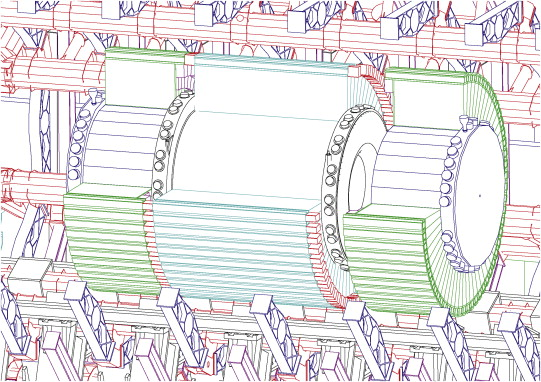
\includegraphics[scale=0.51]{tile_calorimeter.png}} \hspace{0.5cm}
\subfloat[][]{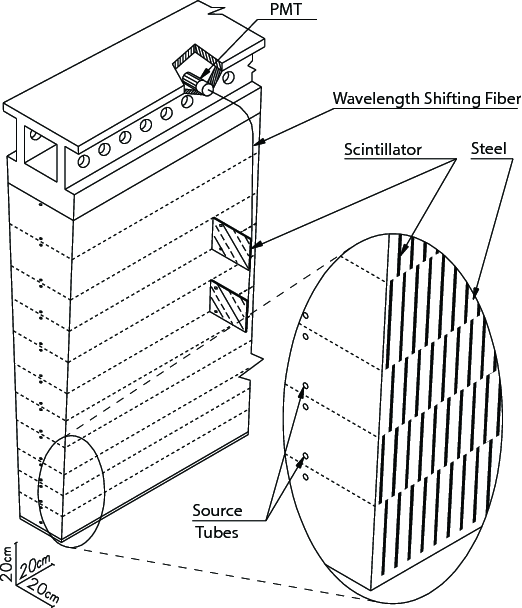
\includegraphics[scale=0.21]{TileCal_Module.png}}
\caption{a)Split figure of Tile Calorimeter, showing both the barrel and two extended barrel sections; b)Mechanical structure of a calorimeter's module.}
\label{TiLe_modules}
\end{figure}

\subsection{The Forward Calorimeter}
The Forward Calorimeter (FCal) \cite{Artamonov_2008}, placed near the incident beams at 4.7 m from the interaction point, complete the nearly $4\pi$ sterad coverage for high $p_T$ particles resulting from proton-proton collisions in the ATLAS detector.
\\
The Forward Calorimeter covers the pseudorapidity range $3.1 < |\eta| < 4.9$ and provides measurements of both electromagnetic and hadronic showers. For this purpose this calorimeter is segmented into different parts, each of them expecially designed for the one or the other shower. In particular, the electromagnetic segment uses Copper as absorber material and Liquid Argon (LAr) as active medium, while the hadronic segment is made of Tungsten as absorber, letting the Liquid Argon as sensitive material.
\\
Since the FCal is placed so close to the incident beams, the jets seen in the detector typically are of high energy. For that reason, the effective energy resolution, parametrized as \cite{Archambault_calibration}
\begin{equation}
\frac{\sigma_E}{E} = \frac{a}{\sqrt{E}} \oplus c
\end{equation}
is dominated by the constant term, where
\begin{equation}
\frac{\sigma_E}{E} = \frac{(28.5 \pm 1.0)\%}{\sqrt{E}} \oplus (3.5 \pm 0.1)\%
\end{equation}
was measured for electrons and
\begin{equation}
\frac{\sigma_E}{E} = \frac{(94.2 \pm 1.6)\%}{\sqrt{E}} \oplus (7.5 \pm 0.4)\%
\end{equation}
for pions, between 20GeV and 200 GeV.
\\
In order to study the longitudinal shower development, the FCal is divided into three different sections, visible in Fig.\ref{FCal}. In all of the three sections only radiation hard materials are used, and there are no adhesive used in joints. FCal1 is designed to detect electromagnetic showers, while FCal2 and FCal3 are denser and serve to stop and collect the energy released in the hadronic showers.
\begin{figure}[h]
\centering
\subfloat{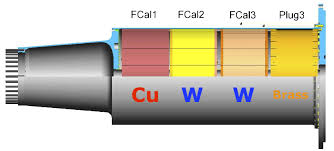
\includegraphics[scale=0.55]{atlas_fcal.jpeg}}
\subfloat{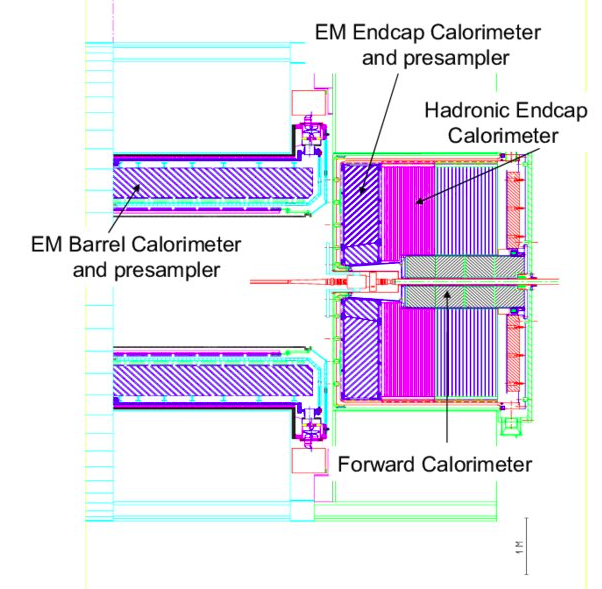
\includegraphics[scale=0.2]{fcal_position.png}}
\caption{The general arrangement of the Forward Calorimeter.}
\label{FCal}
\end{figure}

\section{The Muon Spectrometer}
Most of the particles produced in a collision are absorbed by either electromagnetic or hadronic calorimeter. The only particles which exceed all the layers of the detector are neutrinos and muons. If the only way to detect neutrinos is the missing energy's analysis because they don't interact with any of the layers, muons are detected by the Muon Spectrometer (MS) \cite{CERN-LHCC-97-022}, the last ATLAS layer.
\\\\
The purpose of this detector is the high-precision measurement of the muon momentum, involving the magnetic deflection of the muon tracks, caused by the toroidal magnetic field. The Muon Spectrometer is divided into three parts, a central barrel closed by two end-caps, covering the pseudorapidity range $|\eta| < 2.7$, except for a small region $|\eta| < 0.1$ needed by the services for the inner detectors. In the region $1.0 < |\eta| < 1.4$, referred to as transition region, the magnetic deflection is provided by a combination of barrel and end-cap fields, making the field mostly orthogonal to the muon trajectories.
\\\\
The muon trajectories are bended by the magnetic field in the ($R$, $z$) plane, using two different systems to measure the hits. In the barrel region, tracks are measured in three cylindrical chambers concentric with the beam axis, while in the transition and end-cap regions the three chambers are installed vertically. Different types of detectors are used in the various regions: Monitored Drift Tubes (MDTs) in the barrel cover $|\eta| < 2.7$ and Cathode Strip Chambers (CSCs) in the forward region cover $2.0 < |\eta| < 2.7$.
\\
Each MDT's chamber is made of 3-8 layers of drift tubes filled with a non-flammable Ar-CH$_4$-N$_2$ at 3 bar absolute pressure and with an average single-wire resolution of 80 $\mu$m and 35 $\mu$m per chamber. The tube lengths vary from 70 cm to 630 cm.
\vspace{0.5cm}
\begin{figure}[b!]
\centering
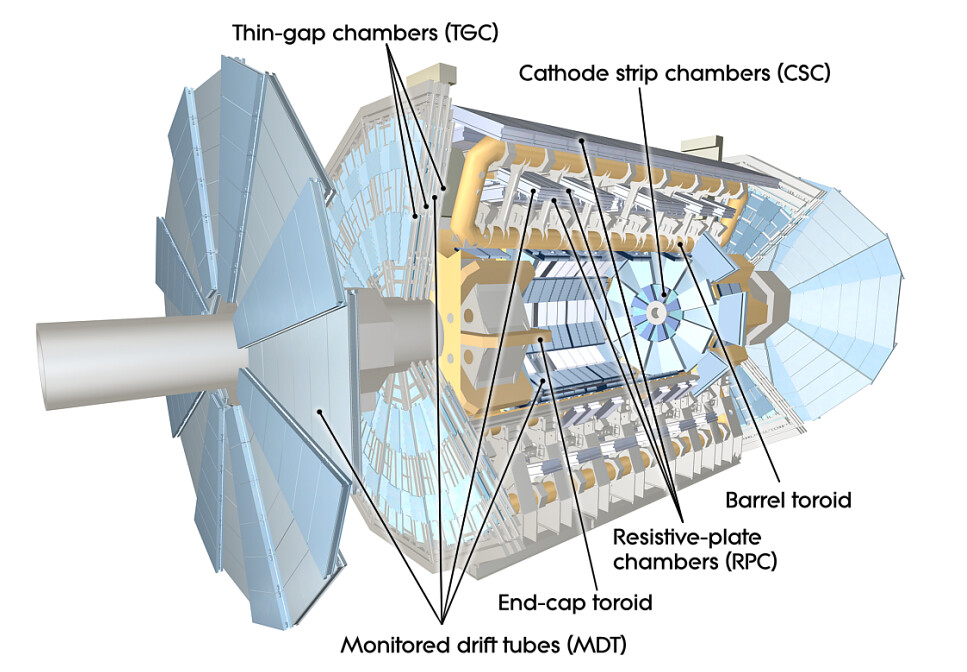
\includegraphics[scale=0.45]{muon_spectrometer.jpg}
\caption{Cut view of the Muon Spectrometer system.}
\end{figure}
\\The Cathode Strip Chambers, differently from MDTs, are multiwire proportional chambers optimized to have the wires oriented in the radial direction. The precision coordinate is obtained by measuring the charge induced on the segmented cathode by the avalanche formed on the anode wire. This design allows to have a resolution of 60 $\mu$m in the bending plane and 4 mm in the transverse plane. Other important characteristics are small electron drift times ($\leq 30$ ns), good time resolution (7 ns), good two-tracks resolution and low neutron sensitivity.
\\\\
The ATLAS Muon Spectrometer system, in particular the Monitored Drift Tubes, provides a momentum resolution between 2-3\% an $\sim$10\% in a $p_T$ range between 10 GeV and 1 TeV. 
\chapter{Physics objects reconstruction with ATLAS detector}
\label{capitolo_4}
The starting point for every physics analysis at the ATLAS experiment is to recognize and distinguish the different types of particles arising from proton-proton collisions, relying on the informations from the sub-detectors.
\\
Because of the high LHC luminosity and the consequently high pile-up events, a strong identification algorithm, peculiar for each physical object to identify, is required.

\section{Electrons and photons reconstruction}
Stable particles that interact primarily via the electromagnetic interaction, such electrons or photons, are found in many final states of proton-proton collisions at LHC.
\\
Electrons and photons identification \cite{ATL-PHYS-PUB-2011-006, ATL-PHYS-PUB-2011-007} is of wide interest in the background rejection. The reconstruction is designed to separate electrons, converted photons in the detector materials to electron-positron pairs and unconverted photons:
\begin{itemize}
\item Clusters with matching tracks related to secondary vertices compared to the interaction one are classified as converted photon candidates;
\item Clusters not related to any matching track in the Inner Detector are considered as unconverted photon candidates;
\item If a track matching the primary vertex is found, which is not related to any photon conversion process, it can be flagged as an electron candidate.
\end{itemize}
The reconstruction of electrons and photons starts from the tracks reconstruction in the Inner Detector and clusters in the Electromagnetic Calorimeter. Technically speaking, tracks in the Inner Detector are used to reconstruct secondary vertices which cna be due to photon conversion.

\subsection{The calorimeters' energy clusters and clustering algorithms}
Starting points of the particle reconstruction in the central $|\eta| < 2.47$ region of the ATLAS detector are the deposits in the Electromagnetic Calorimeter. The geometry of the calorimeter allows to collect the energy released by using a very dense grid of elements, known as cells, merging them into clusters to include the electromagnetic shower induced by the incoming particle.
\\\\
In the clustering process a new algorithms are used, in order to provide inputs for particle identification.
\\\phantom{1}\hspace{0.3cm} The \emph{slinding-window} \cite{Lampl_1099735} kind of algorithms build clusters summing energy towers within a fixed-size rectangular window and differ size in order to maximise the efficiency for different particle identification: electromagnetic, generally used for electrons and photons, and combined for jet finding principally, including informations from the Electromagnetic as well as the Hadronic calorimeters. The tower clustering algorithm starts with the tower building, proceding with precluster finding and cluster filling. For electromagnetic clusters the precluster finding and the cluster filling occur in a single step, while for combined clusters they are actually spread in two separate steps. The $\eta - \phi$ space of the calorimeter is divided into a grid of $N_{\eta} \times N_{\phi}$ elements, each one of size $\Delta \eta \times \Delta \phi$. The energy released into all cells in all longitudinal layers is summed into the \emph{tower} energy.
\begin{table}[h]
\caption{Configuration of tower building's parameters for the two type of algorithms.}
\begin{center}
\begin{tabular}{ l | c | c }
  \hline			
  Tower Type & Electromagnetic & Combined \\
  \hline
  Calorimeters & EMB, EMC & All \\
  \hline
  $|\eta_{max}|$ & 2.5 & 5.0 \\
  \hline
  $N_{\eta}(\Delta \eta)$ & 200(0.025) & 100(0.1) \\
  \hline  
  $N_{\phi}(\Delta \phi)$ & 256(0.025) & 64(0.1) \\
  \hline
\end{tabular}
\end{center}
\end{table}
\\A moving window of fixed size $N_{\eta}^{\text{window}} \times N_{\phi}^\text{window}$ slides across each cell of the detector's grid, measuring the sum of the transverse energy of  the towers contained into the window. If the transverse energy value of the selected window lies above a certain threshold $E_{T}^{thresh}$ and it is considered a local maximum too, a precluster is formed.
\\\\
To maximize the efficiency in the precluster finding and to contain the rate of fake preclusters due to noise simultaneously, the size of the window and the energy threshold are differently optimized: the dimension of the cluster should be large enough in order to include most of the energy profile of the electromagnetic shower, but increasing the size of the cluster means more electronic and more pileup noise. Once the precluster is formed, its position is computed evaluating the energy-weighted $\eta$ and $\phi$ baricenters for all cells within a fixed $N_{\eta}^{\text{pos}} \times N_{\phi}^\text{pos}$ size sub-window around the tower at the center of the sliding window. Using a smaller window for the center position's screening makes the computation less sensitive to noise. To increase the efficiency in the data acquisition, if two preclusters have position within a $\Delta \eta_{\text{dupl}} \times \Delta \phi_{\text{dupl}}$ size window, only the precluster with the largest transverse energy is kept, while the other is removed.
\begin{table}[h]
\caption{Parameters for precluster finding, using the sliding-window algorithm. The values are given in units of the tower size $\Delta \eta \times \Delta \phi$.}
\begin{center}
\begin{tabular}{ l | c | c }
  Cluster Type & Electromagnetic & Combined \\
  \hline			
  $N_{\eta}^{\text{window}} \times N_{\phi}^\text{window}$ & $5 \times 5$ & $5 \times 5$ \\
  $E_{T}^{thresh}$ (GeV) & 3 & 15 \\
  $N_{\eta}^{\text{pos}} \times N_{\phi}^\text{pos}$ & $3 \times 3$ & $3 \times 3$ \\
  $\Delta \eta_{\text{dupl}} \times \Delta \phi_{\text{dupl}}$ & $2 \times 2$ & $2 \times 2$
\end{tabular}
\end{center}
\end{table}
\\The shape and the granularity of each cluster for both $\eta$ and $\phi$ coordinates are differently optimized in the barrel and in the end-caps electromagnetic calorimeters, considering the selected particle and the physical processes undelying in the passage through the detector: in the barrel, shower arising from electrons are wider than those arising from photons because the former interact more with the materials, being able to emit in this way bremsstrahlung photons. Since the magnetic field curves the electrons' tracks in the $\phi$ direction, the $\phi$ size of the cluster is adjusted in order to contain most of the released energy. In the same way, converted photons produce $e^+e^-$ pairs, which are oppositely curved by the magnetic field and spread along the $\phi$-axis. In the end-caps calorimeters things are simpler because the cluster size is the same for all particles, due to the smaller effect of the magnetic field induced on the particles. It is larger in $\eta$ than in the barrel because of the smaller physical cell size. The efficiency of the cluster search varies from 96\% at $E_T = 7$ GeV to more than 99\% for $E_T > 15$ TeV.
\begin{figure}[b!]
\centering
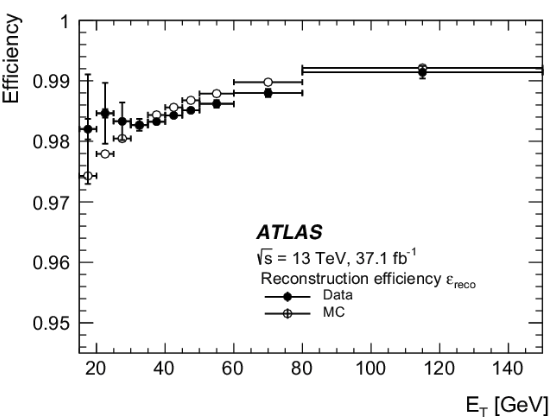
\includegraphics[scale=0.45]{eff_clustering.png}
\caption{The reconstruction efficiency relative to reconstructed clusters, reco, as a function of electron transverse energy $E_T$ for $Z \rightarrow ee$ events, comparing data (closed circles) with simulation (open circles).}
\end{figure}
\\\phantom{1}\hspace{0.3cm} The \emph{topological clustering} \cite{ATL-PHYS-PUB-2017-022} is the other principal approach in the cells clustering process, whose basic idea is to group into clusters neighboring cells, which have significant energies compared to the expected background noise. This approach produces clusters, generally known as \emph{topo-clusters}, with a variable number of cells. The main parameter in seed finding and topo-clusters formation is the cell significance $\zeta_{\text{cell}}^{\text{EM}}$, defined as signal to noise ratio
\begin{equation}
\zeta_{\text{cell}}^{\text{EM}} = \Bigl|\frac{E_{\text{cell}}^{\text{EM}}}{\sigma_{\text{noise}}^{\text{EM}}}\Bigr| \hspace{0.5cm} \text{,}
\end{equation} 
where $E_{\text{cell}}^{\text{EM}}$ is the cell energy at the EM scale and $\sigma_{\text{noise}}^{\text{EM}}$ is the expected cell noise. Cells with an energy significance above an energy threshold $E_{\text{seed}}^{\text{thresh}}$ will be the seeds for clusters formation. Starting from the seed, neighboring cells are included in the cluster if their significance is above a second energy threshold $E_{\text{cell}}^{\text{thresh}}$, generally lower than $E_{\text{seed}}^{\text{thresh}}$ or can serve as an additional seed to expand the cluster if it's above a third medium energy threshold $E_{\text{neighbor}}^{\text{thresh}}$. The hierarchy in the thresholds ensures to not discard the tails of the showers and increasing the efficiency in the suppression of both electronic and pile-up background noise in seed finding process simultaneously.
\begin{table}[h]
\caption{Parameters used to build the two types of topological cluster available in the standard ATLAS reconstruction.}
\begin{center}
\begin{tabular}{ l | c c }
  Parameters & Electromagnetic 633 \\
  \hline			
  Calorimeters & EM only \\
  Seed signal definition & $E$ \\
  $E_{\text{seed}}^{\text{thresh}}$ & 6 \\
  $E_{\text{neighbor}}^{\text{thresh}}$ & 3 \\
  $E_{\text{cell}}^{\text{thresh}}$ & 3
\end{tabular}
\end{center}
\end{table}
\\In the ATLAS reconstruction process, the Electromagnetic "6.3.3" scheme can be used to reconstruct electromagnetic clusters significantly higher than the noise. 
\begin{figure}[htb]
\centering
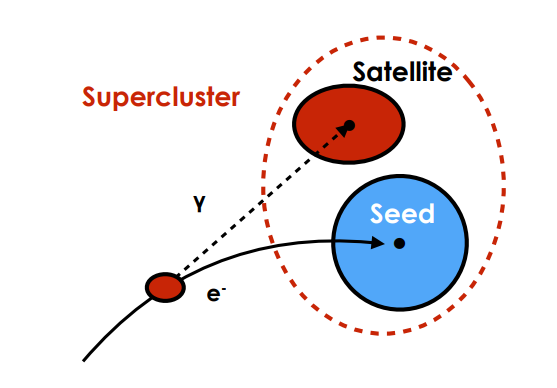
\includegraphics[scale=0.38]{supercluster.png}
\caption{Example of a supercluster, showing a seed electron cluster related with a satellite photon cluster.}
\label{supercluster}
\end{figure}
The real upgrade in the topo-cluster approach is the ability to recover low-energy photons radiated due to bremsstrhalung interactions and connect them to their associated electron or converted photon, forming a so-called \emph{supercluster} (Fig.\ref{supercluster}) \cite{ATL-PHYS-PUB-2017-022} made of a primary \emph{seed} topo-cluster arising from the electron shower and secondary \emph{satellite} topo-clusters.
\begin{figure}[b!]
\centering
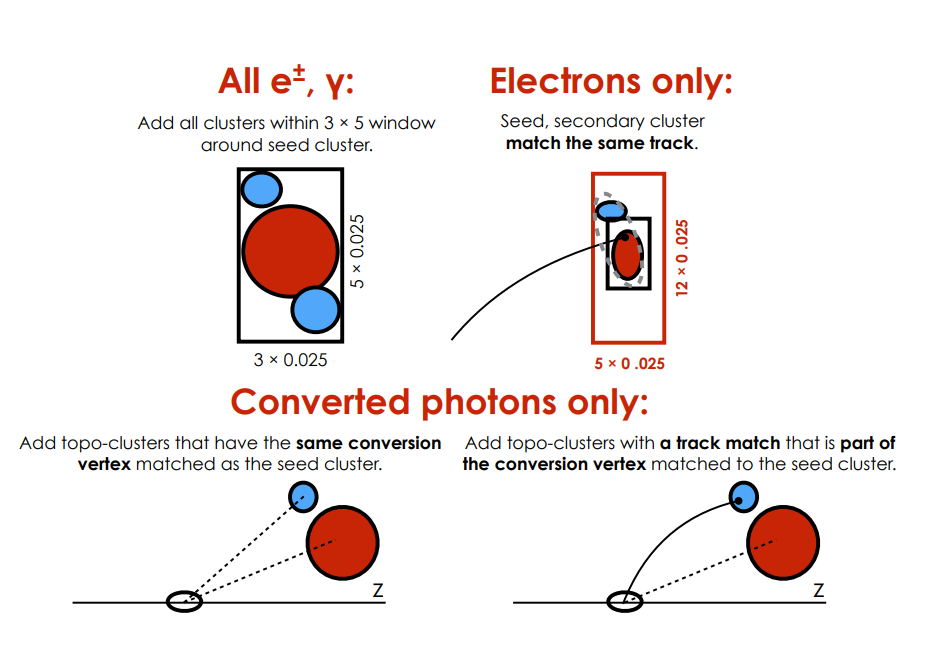
\includegraphics[scale=0.37]{satellite_cluster.png}
\caption{Satellite finding process for different cases.}
\label{satellite}
\end{figure}
\\To form a supercluster, the first step is to select topo-clusters with peculiar requests for either electrons or photons and consider them as the seeds of the superclusters: to become a supercluster seed, an electron-candidate topo-cluster is required to have a minimum energy of 1 GeV and must match tracks with at least four hits in the silicon tracking detector, while a photon-candidate topo-cluster must have a minimum energy greater than 1.5 GeV to compensate the absence of matching tracks.
\\\\
Once the superclusters seeds are selected, the satellite finding step begins, where all of the unused clusters are scanned again in order to associate them to the seed clusters.
\\
In the satellite finding process, both for electrons and photons, a cluster is considered satellite if it falls within a window of $\Delta \eta \times \Delta \phi = (0.075 \times 0.125)$ around the seed cluster barycenter, tenting to parametrize secondary electromagnetic showers  originating from the same initial electron or photon.
\\
Once all of the satellite clusters have been matched with a given seed cluster, the algorithm restart on the unused clusters, until all superclusters are formed.
\\\\
Thanks to the dynamical approach of the topological clustering and the contribution of the satellite clusters from photon bremsstrahlung, the energy collected in the single supercluster is the 96\% of the generated energy, against the 77\% collected in the single sliding-window type cluster. Due to this boost in the accurancy for energy collection, an improvement in resolution up to 20-30\% is found in some end-cap regions' bins, making the topological clustering the algorithm principally used in the actual ATLAS analyses.
\begin{figure}[h]
\centering
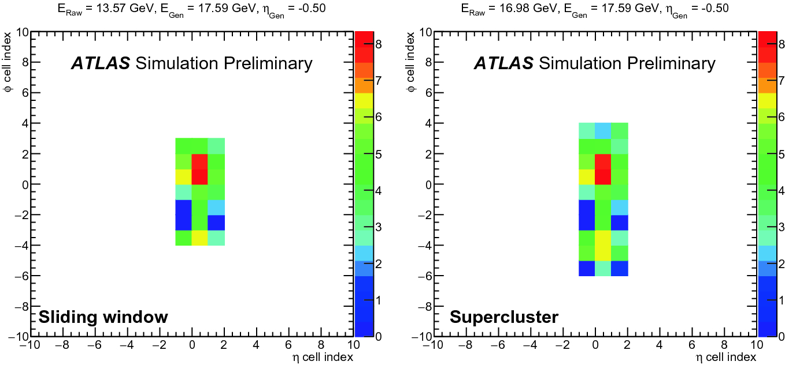
\includegraphics[scale=0.4]{cluster_comparison.png}
\caption{Example of an electron cluster for sliding window (left) and supercluster (right) algorithm}
\end{figure}

\subsection{Electron reconstruction}
The reconstruction of electron candidates within the kinematic region is based on three fundamental elements, characterizing the signature of electrons \cite{Aaboud_2019ynx}: the presence of charged-particle tracks identified in the Inner Detector, localised clusters of energy deposits found in the Electromagnetic Calorimeter and close matching in $\eta \times \phi$ space of the tracks to the clusters to form the final electron-candidate cluster.
\\
Once seed clusters are defined in the Calorimeter, a scan for the corresponding reconstructed tracks in the Inner Detector loosely matched with the clusters begins. A track is considered loosely matched with an energy deposit cluster if the difference in the $(\eta - \phi)$ coordinates with the seed cluster barycenter is below 0.05 along $\eta$- and $\phi$-axis in the direction of the bending of the tracks as a consequence of the magnetic field's effect or within 0.2 in the opposite direction.
\\\\
More constraints can be applied at the electron candidates, such as a tighter request $\Delta \phi < 0.1$ in the direction of the bending of the tracks. If more than one track matches with the same seed cluster, just the track with the smallest $\Delta R$ withe the calorimetic cluster is selected. In cases where the difference between $\Delta R$ of the tracks are $<0.01$, the track with more hits in the trajectory is chosen, to improve the track-reconstruction resolution. Once matched, informations from Inner Detector's tracks and from Electromagnetic Calorimeter clusters help to compute the four-momentum of the electron candidate: the energy of the particle is given by the energy deposits released in the calorimeter, while the trajectory is extrapolated from the hits in the pixel detectors.
\\\\
In order to reduce the background noise deriving from photon conversions and other secondary particles, the electron candidates must be compatible with the interaction vertex and undergo fixed requirements on tracking criteria: the Loose, the Medium and the Tight criteria require at least two hits in the pixel detector and seven in total concerning pixel and sylicon strip detectors combined. For the Medium and Tight criteria, also, one of the pixel hits must be in the innermost pixel layer.
\begin{figure}[h]
\subfloat{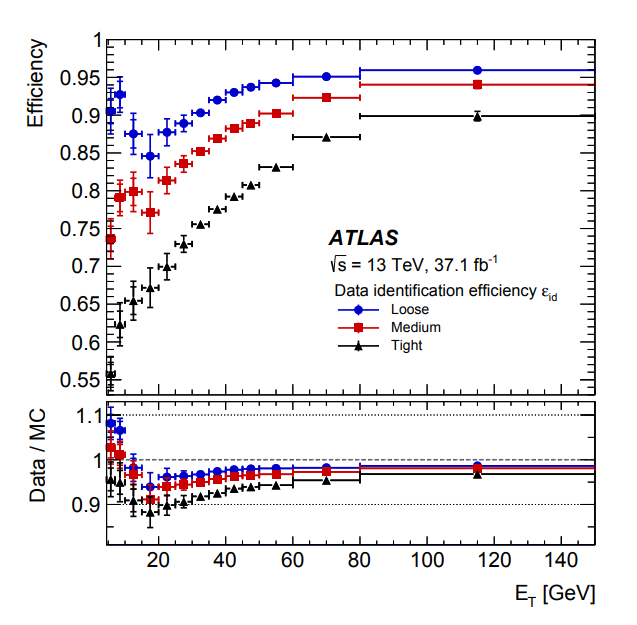
\includegraphics[scale=0.32]{eff_electron_1.png}}
\subfloat{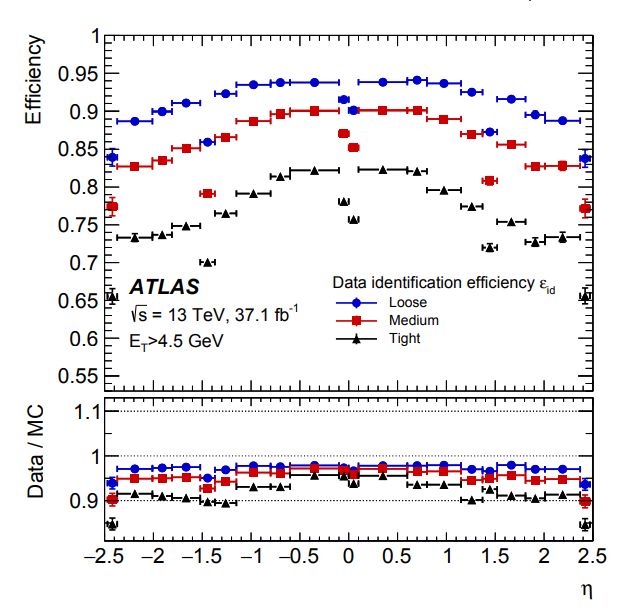
\includegraphics[scale=0.32]{eff_electron_2.png}}
\caption{Measured LH electron-identification efficiencies in $Z \rightarrow ee$ events for the Loose (blue circle), Medium (red square), and Tight (black triangle) operating points as a function of ET (top) and $\eta$ (bottom).}
\end{figure}

\subsection{Photon reconstruction}
The photon reconstruction \cite{Aaboud_2016yuq, Aaboud_2018yqu} is pretty similar to the electron reconstruction, with some complications arising from the different photon processes in the detector. For an unconverted photon, in fact, no tracks related to the energy deposit cluster will be present in the Inner Detector, while for a converted photon there will be reconstructed tracks pointing at a secondary conversion vertex. After the crossing of the particle, a sliding window of size $3 \times 5$ in units of $(\Delta \eta \times \Delta \phi) = (0.025 \times 0.0245)$\footnote{The sliding window size is optimized to fit with the Electromagnetic Calorimeter's granularity of the middle layer.}
is used to search for the electromagnetic cluster seeds with total cluster transverse energy above 2.5 GeV.
\\
Once the seeds are found the clusters are formed using the topological clustering algorithm, removing the duplicates too. The cluster kinematics is reconstructed through an extended window depending on the cluster's position in the calorimeter. With this procedure, the efficiency of the photon cluster formation in simulation is higher than 99\% with $E_T > 20$ GeV.
\\\\
To reconstruct converted photons also information from the Inner Detector can be used, searching for reconstructed tracks loosely matched to seed clusters: these tracks will be used as inputs for the reconstruction of the secondary conversion vertex. Reconstructed conversion tracks can be distinguished between tracks with silicon hits, referred to as \emph{Si-tracks}, and tracks with Transition Radiation Tracker (TRT) hits, known as \emph{TRT-tracks}, while a vertex can be reconstructed as single-track or double-tracks conversion vertex. The single-track vertices are built with tracks with no hits in the innermost layer, while two-tracks vertices arise from two tracks forming a vertex consistent with that of a massless particle. In the case of multiple conversion vertices point at a single cluster, double-tracks conversions with two silicon tracks are generally preferred.
\begin{figure}[t]
\centering
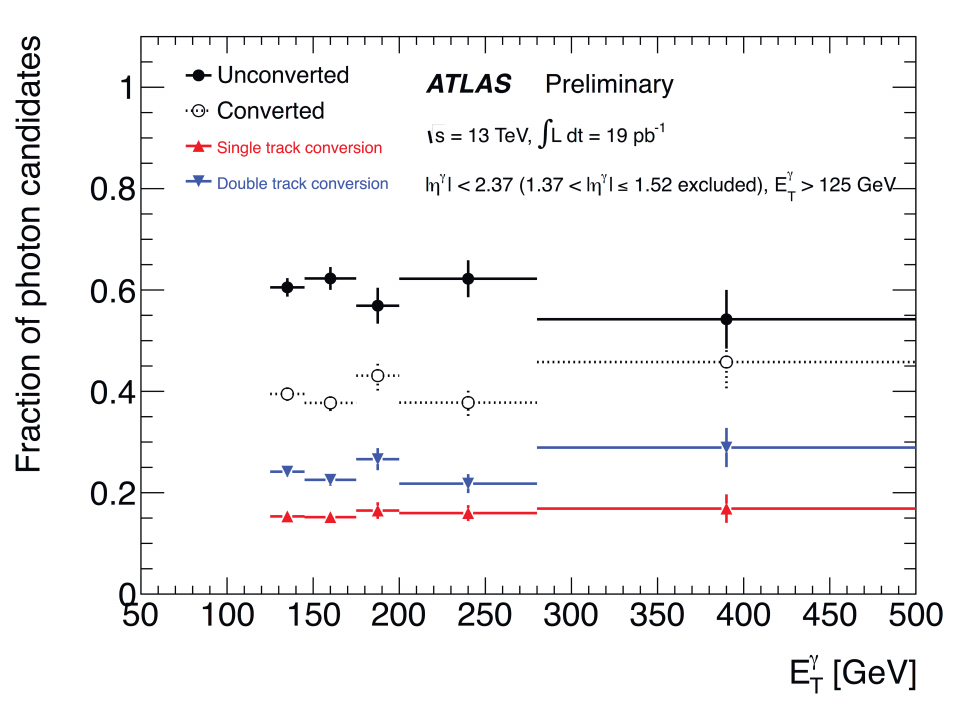
\includegraphics[scale=0.27]{fraction_photons.png}
\caption{Fraction of photons candidates, as a function of the candidate transverse momentum, reconstructed as unconverted or converted photons, switched in one- or two-tracks reconstruction.}
\end{figure}
\\Without any combination with the Inner Detector informations, the calorimetric clusters can be considered as photon or as electron candidate at the same time. The final distinction between the various cases is performed using a series of requirements to distinguish the detected process:
\begin{itemize}
\item a candidate reconstructed particle is named as an unconverted photon if there are no tracks with at least four hits in the silicon detector pointing to the calorimetric cluster. A converted photon, in the other way, is where a double-silicon conversion vertex is found and one of the tracks arising from that vertex is flagged as an electron without any hits in the pixel detector;
\item a candidate particle is reconstructed as an electron if the track is related with the primary vertex and it has at least two hits in the pixel detector and four hits in the silicon detector. In the case of an electron deriving from a secondary conversion vertex, the vertex is not a double-silicon tracks vertex or, in that case, just one of the reconstructed conversion tracks has innermost pixel hits;
\item the worst scenario is when a particle can be reconstructed both as photon and as electron. That is the case of particle not fulfill the previous requirements or the track transverse momentum is smaller than 2 GeV.
\end{itemize}

\section{Photon identification and isolation}
Several processes in LHC proton-proton collisions are related with the production of final states with \emph{prompt photons}, namely photons not originating from hadrons' decays, which are known as \emph{background photons}. The main contribution to the inclusive cross section consists of photons production, in association with jets, such as $q\bar{q} \rightarrow \gamma + X$, or production of photons pairs, such as $q\bar{q} \rightarrow \gamma \gamma$. As well as these kind of events, but with a pretty smaller cross section, other rarer events may produce a prompt photons pair, like the di-photon decay channel of the Higgs boson.
\\\\
From kinematics considerations, turns out how each event requires differently orientated photons. The observable called \emph{isolation} quantifies the presence of additional secondary particles around the photon candidate, improving in this way the jet-background rejection of the photon selection. For the diphoton Higgs decay, object of this work, two isolated photons are requested.

\subsection{Photon identification}
The photon identification process is based on independent requirements related to the calorimetric variables, which carries a good separation efficiency between prompt photons and background arising from jets. They can be grouped in three main categories, each one considering a different aspect of the detector: hadronic leakage variables, relying informations about the hadronic calorimeter, variables using the second longitudinal compartment of the Electromagnetic Calorimeter, and variables using the first layer of the same calorimeter.
\\\\
In the photon identification process, two kinds of selection are defined: the \emph{loose} and the \emph{tight} selection. The loose selection criteria are based on the informations collected from the electromagnetic calorimeter's second layer and from the hadronic leakage. This selection has been optimized to maximize the photon identification efficiency from 97\% for photons with $E_T = 20$ GeV up to 99\% for $E_T > 40$ GeV. The loose selection is typically used to define control regions enriched of background events and as a preliminary selection to prune the raw data. 
\\\\
In the tight selection all of the identification variables are used, making the prompt photon identification quite more precise. With these criteria, peculiar phenomena, such as the two separated maxima of the collimated photons arising from the $\pi^0$ decay, can be distinguished, improving the rejection against $\pi^0$ particles. The peculiar signatures of unconverted and converted photons impose a different optimization for the tight selection criteria, providing a photon identification efficiency of 85\% for photons with $E_T > 40$ GeV.
\begin{table}[t]
\centering
\caption{Discriminating variables used for \emph{loose} and \emph{tight} photon identification}
\small
\begin{tabular}{l|l|l|l|l}
\thead{Category} & \thead{Description} & \thead{Name} & \thead{\emph{loose}} & \thead{\emph{tight}} \\
\hline
Acceptance & $|\eta| < 2.37$, with $1.37 < |\eta| < 1.52$ excluded & $-$ & $\bullet$ & $\bullet$ \\
\hline
\multirow{2}{*}{\makecell{Hadronic\\ Leakage}} & \makecell{Ratio between $E_T$ in the first sampling\\ layer of the hadronic calorimeter and\\$E_T$ of the EM cluster} & $R_{\text{had1}}$ & $\bullet$ & $\bullet$ \\
\cline{2-5}
& \makecell{Ratio between $E_T$ in the hadronic\\ calorimeter and $E_T$ of the electromagnetic\\ cluster} & $R_{\text{had}}$ & $\bullet$ & $\bullet$ \\
\hline
\multirow{3}{*}{EM \ordinalnum{2} layer} & \makecell{Ratio between $3 \times 7$ and $7 \times 7$\\ in $\eta \times \phi$ cell energies} & $R_{\eta}^{3 \times 7}$ & $\bullet$ & $\bullet$ \\
\cline{2-5}
& Lateral shower width & $w_{\eta 2}$ & $\bullet$ & $\bullet$ \\
\cline{2-5}
& \makecell{Ratio between $3 \times 3$ and $7 \times 7$\\ in $\eta \times \phi$ cell energies} & $R_{\phi}^{3 \times 3}$ & $-$ & $\bullet$ \\
\hline
\multirow{5}{*}{EM \ordinalnum{1} layer} & \makecell{Shower width calculated from three strips\\ around the strip with the maximum\\ energy deposit} & $w_{s3}$ & $-$ & $\bullet$ \\
\cline{2-5}
& Total lateral shower width & $w_{s\text{tot}}$ & $-$ & $\bullet$ \\
\cline{2-5}
& \makecell{Energy outside the core of the three\\ central strips but within seven strips\\ divided by the energy within the\\ three central strips} & $F_{\text{side}}$ & $-$ & $\bullet$ \\
\cline{2-5}
& \makecell{Difference between the energy associated\\ with the second maximum in the strip\\ layer and the energy reconstructed in the\\ strip with the minimum value found\\ between the first and the second maxima} & $\Delta E$ & $-$ & $\bullet$ \\
\cline{2-5}
& \makecell{Ratio of the energy associated\\ with the largest and second largest energy\\ deposits to the sum of these energies} & $E_{\text{ratio}}$ & $-$ & $\bullet$ \\

\end{tabular}
\end{table}
\\\\The efficiency of the tight photon identification criteria
\begin{equation}
\mathlarger{\mathlarger{\varepsilon}}_{\text{ID}} = \frac{N_{\gamma}^{\text{iso, pass}}}{N_{\gamma}^{\text{iso, tot}}}
\end{equation}
is, in this way, the number of isolated photons passing the tight selection against the total number of isolated photons.
\\
To evaluate the efficiency from data  using three main methods are used, covering a very wide energy range:
\begin{itemize}
\item the first method uses a pure sample of photons selected from leptonic radiative decay of the $Z$ boson, $z \rightarrow l^+l^- \gamma$, $l = e, \mu$, and brings a precise measurement of $\varepsilon_{ID}$ in the low-$E_T$ region $10 \text{GeV} \lesssim E_T \lesssim 100 \text{GeV}$;
\item the second method, generally known as \emph{electron extrapolation}, is based on an electron sample selected from the $Z$ boson $Z \rightarrow e^+e^-$ decays in order to obtain a pure sample of electromagnetic shower shapes from data. This method allows to investigate an $E_T$ region of $30 \text{GeV} \lesssim E_T \lesssim 100 \text{GeV}$;
\item the third method, called \emph{inclusive photon}, makes use of matrix method to determine the number of prompt photons in a control region before and after the application of the tight selection criteria. Using this method, the very wide energy range of $20 \text{GeV} \lesssim E_T \lesssim 1.5 \text{TeV}$ is covered.
\end{itemize}

\subsection{Photon isolation}
In order to reduce the main background source coming from photons emitted from high-$p_T$ $\pi^0$ decays in jets, some experimental isolation conditions on selected photons are needed. These requirements exploit the Electromagnetic Calorimeter and the Inner Detector in the direction of performing studies on the transverse energy deposited in the calorimeter and on the reconstructed tracks nearby to the photon candidate.
\\\\
The transverse isolation energy $E_T^{\text{iso}}$, defined as the scalar sum of the energy in both the Electromagnetic and Hadronic calorimeter's cells within a cone of radius 0.4 centered around the photon candidate, is computed starting from the three-dimensional topo-clusters falling within the Isolation Cone. A rectangular $5 \times 7$ Core interval around the photon candidate barycenter is then removed from the isolation energy $E_T^{\text{iso}}$ computation, in order to not include the photon energy. An additional correction is applied to remove the contribution of the photon isolation energy fraction which leaks out of the core. Once the last correction is computed, the isolation energy $E_T^{\text{iso}}$ is nominally independent of the photon transverse energy. In order to remove the pile-up and underlying event contribution, other corrections to $E_T^{\text{iso}}$ must be applied.
\\\\
Other information concerning photon isolation come from the reconstructed tracks in the Inner Detector. The track isolation $p_T^{\text{iso}}$ is computed by summing the transverse momenta of the tracks with $p_T > 1$ GeV falling into a different isolation cone, centered around the photon direction. The selected tracks need to be compatible with originating from the primary interaction vertex in order to limit the pile-up contribution, while the contribution of the tracks arising from converted photons are removed not considering in the $p_T^{\text{iso}}$ computation tracks extrapolated from a selected window around the photon topo-cluster in the Electromagnetic Calorimeter \ordinalnum{2} layer.
\begin{figure}[b!]
\hspace{1.5cm}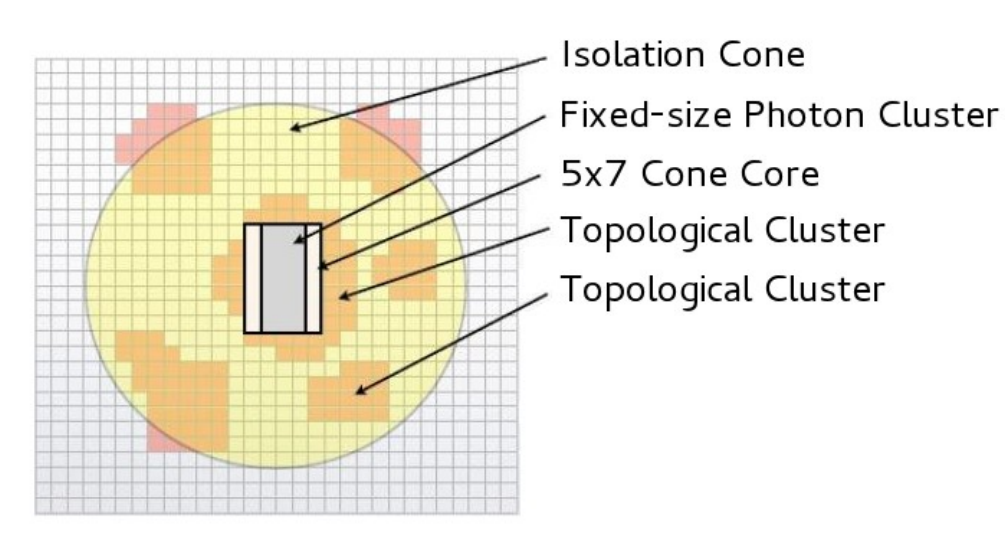
\includegraphics[scale=0.33]{photon_isolation.png}
\caption{Calorimeter's photon isolation method. The grid is in the $\eta - \phi$ space.}
\end{figure}

\section{Jet reconstruction}
Once a gluon or a quark is produced in a collision, they immediately hadronize just after their production\footnote{Both quarks and gluons hadronize immediately, except for the $t$-quark, which decays before hadronize, due to it extremely heavy mass. It is, so far, the only chance to investigate a quark as a free particle.}
and produce sprays of hadrons, called \emph{jets}. Since they are not a single physical entity, hadronic jets are very sensitive to the clustering algorithm used in the analysis. In the ATLAS experiment, the clustering algorithm used for jets is the \emph{anti-}$k_t$ algorithm \cite{Cacciari_2008}, starting from the three-dimensional energy clusters of the calorimeter's cells. By using simulations, the calorimeter response to the reconstructed jets is calibrated using a $p_T$- and $\eta$-dependent factor \cite{Collaboration2017JetES}, while the pile-up contribution is hardly removed applying a jet-area-dependent correction \cite{2013PileupSA}.
\\\\
After the jet clustering process, new and different requirements, generally known as \emph{jet cleaning criteria}, are used to maximize the rejection of the background arising from non-collision reconstructed jets and instrumental noise. The pile-up background contribution is suppressed applying a lower limit on the \emph{Jet Vertex Fraction} (JVF) \cite{ATLAS-CONF-2014-018}. This variable's cut helps to reject the most of pile-up jets, but it is strongly dependent on the number of primary vertices in the event. 
\chapter{Higgs boson fiducial cross sections in the $H \rightarrow \gamma\gamma$ channel}
\label{capitolo_5}
In this section the differential cross sections for Higgs boson decaying production into the two-photons channel are measured, using 139 fb$^{-1}$ of full Run2 proton-proton collisions recorded at a center-of-mass energy of $\sqrt{s} = 13$ TeV by the ATLAS experiment at the Large Hadron Collider during the period 2015-2018. Analyses with smaller dataset at center-of-mass energy of $\sqrt{s} = 13$ TeV for both ATLAS and CMS experiments are in \cite{Aaboud_measurements, collaboration2018MeasurementAI}. The differential cross section measurements are separately performed for a set of variables, considering several quantities of the di-photon system and the jets kinematics and of the jets multiplicity produced with the Higgs boson\footnote{No separation has been done distinguishing the Higgs boson production modes. Actually the measured cross sections are inclusive in the production.}. 
The variables used in this work are presented down below:
\begin{itemize}
\item $p_T^{\gamma\gamma}$: The transverse momentum of the Higgs boson, measured with the di-photon system;
\item $|y_{\gamma\gamma}|$: The absolute rapidity of the Higgs boson, measured with the di-photon system;
\item $N_{\text{jets}}^{30}$: The multiplicity of jets associated with the Higgs boson production;
\item $p_T^{j1, 30}$: The transverse momentum of the highest-$p_T$ leading jet;
\item $m_{jj}^{30}$: The invariant mass of the two leading jets;
\item $\Delta \phi_{jj}$: The azimuthal angular difference of the two leading jets.
\end{itemize}
The flag '$30$' stands for the requirement for jets to have $p_T > 30 \text{GeV}$ to be selected for the analysis. The binning intervals for each quantity in the analysis is shown in Table \ref{binning_table}.
\\
The $p_T^{\gamma\gamma}$ distribution is sensitive to the bottom and charm quark Yukawa couplings of Higgs boson \cite{Bishara_2017}, while in the high-transverse-momentum region has a sensitivity to new heavy particles coupling to the Higgs boson. The $|y_{\gamma\gamma}|$ distribution is particularly responsive to the modeling of the production mechanism and to the parton distribution functions (PDF) of the colliding protons. The $p_T^{j1}$ distribution is sensitive  to the relative contributions of the different Higgs production mechanism, while the $m_{jj}$ distribution has sensitivity to the Vector Boson Fusion (VBF) production mechanism. Finally, the angular variable $\Delta \phi_{jj}$ is sensitive to the spin and CP quantum numbers of the Higgs boson.
\\\\
The measurements are performed in a fiducial region, definited by two isolated photons with transverse momentum greater than 35\% and 25\% of the total diphoton invariant mass for the leading and sub-leading photons respectively, each in a pseudorapidity region of $|\eta| < 1.37$ or $1.52 < |\eta| < 2.37$. Considering moreover the jets-related events, the constraints on jets require to have a transverse momentum $p_T > 30$ GeV and rapidity $|y| < 4.4$. The photon isolation is required to ensure to avoid the jets's fake rate wrongly classified as photons.
\\
The $H \rightarrow \gamma\gamma$ signal yield in each bin of the variable of interest has been extracted from fits to the di-photon invariant mass spectrum, assuming the Higgs boson mass to be $125.09 \pm 0.24$ GeV \cite{Aad_2015}, and the measured cross sections are tuned applying corrections arising from experimental effects and considering the integrated luminosity of the dataset.
\begin{table}[h]
\centering
\small
\caption{Binning intervals for each observable studied in the analysis.}
\label{binning_table}
\begin{tabular}{l | cccccc}
Bin & $p_T^{\gamma\gamma}$ [GeV] & $|y|_{\gamma\gamma}$ & $p_T^{j1, 30}$ [GeV] & $\Delta\phi_{jj}$ & $N_j^{30}$ & $m_{jj}^{30}$ [GeV] \\
\hline
1 & $0-5$ & $0-0.15$ & $<2 \hspace{0.1cm}\text{jets}$ & $-3.15--1.57$ & $= 0$ & $0-170$ \\
2 & $5-10$ & $0.15-0.30$ & $0-30$ & $-1.57-0$ & $= 1$ & $170-500$ \\
3 & $10-15$ & $0.30-0.45$ & $30-60$ & $0-1.57$ & $= 2$ & $500-1500$ \\
4 & $15-20$ & $0.45-0.60$ & $60-90$ & $1.57-3.15$ & $\geq3$ & $1500-\infty$ \\
5 & $20-25$ & $0.60-0.75$ & $90-120$ & - & - & - \\
6 & $25-30$ & $0.75-0.90$ & $120-350$ & - & - & - \\
7 & $30-35$ & $0.90-1.20$ & $\geq350$ & - & - & - \\
8 & $35-45$ & $1.20-1.60$ & - & - & - & - \\
9 & $45-60$ & $1.60-2.40$ & - & - & - & - \\
10 & $60-80$ & - & - &  - & - & - \\
11 & $80-100$ & - & - & - & - & - \\
12 & $100-120$ & - & - &  - & - & - \\
13 & $120-140$ & - & - & - & - & - \\
14 & $140-170$ & - & - & - & - & - \\
15 & $170-200$ & - & - & - & - & - \\
16 & $200-250$ & - & - & - & - & - \\
17 & $250-350$ & - & - & - & - & - \\
18 & $350-\infty$ & - & - & - & - & -
\end{tabular}
\end{table}

\section{Dataset and events simulation}
\label{mc_sim}
The analysis is based on $\sqrt{13}$ TeV proton-proton collisions, recorded from 2015 to 2018 with a proton bunch spacing of 25 ns. Because of the different luminosities reached during the data taking, the average number of interactions per bunch crossing varies from 24 in 2015-2016 to 37 in 2017-2018 data, leading to an average number of interaction per bunch crossing $\mu=34$.Prompt events are selected by using a diphoton trigger with $p_T$ threshold of 35 GeV and 25 GeV for the leading and sub-leading photon candidates respectively. Loose photon identification requirements are applied by the diphoton trigger in the 2015-2016 dataset and upgraded to tight requirements to deal with the higher instantaneous luminosity in the 2017 dataset, bringing the total identification efficiency of the diphoton trigger greater than 98\% for $H \rightarrow \gamma\gamma$ events passing the selections described below.
\\
After the data quality requirements achievement to ensure good working condition for all detector's sub-systems, the final integrated luminosity for the merged dataset settles down to $(139.0 \pm 2.4)$ fb$^{-1}$ \cite{ATLAS-CONF-2019-021}.
\\
The study of the backgroung and signal processes modelling is done using samples produced with MonteCarlo simulations. The background simulation is used to select the best functional form to fit the data and to estimate the systematic uncertainties related to the signal extraction due to the background mismodelling, such as the spurious signal (Section \ref{spur_sign_sec}). The $H \rightarrow \gamma\gamma$ signal simulation, on the other hand, is needed to determine the mass shape and the efficiencies for both \emph{c-factors} method (Section \ref{c_factors_sec}) and \emph{matrix} method (Section \ref{matrix_sec}).
\begin{table}[h]
\caption{MonteCarlo signal samples used in the analysis. The order listed for the QCD and EW calculations refers to the order to which the samples are normalized.}
\label{signal_samples}
\begin{center}
\begin{tabular}{ c | c | c | c}
  Process & Generator & Cross-section normalization & $\sigma \times \text{BR}$[fb] \\
  \hline			
  ggF & P{\scriptsize OWHEG} NNLOPS & N$^3$LO(QCD)+NLO(EW) & 110 \\
  VBF & P{\scriptsize OWHEG}-B{\scriptsize OX} & approx. NNLO(QCD)+NLO(EW) & 8.58 \\
  $W^+H$ & P{\scriptsize OWHEG}-B{\scriptsize OX} & NNLO(QCD)+NLO(EW) & 1.90 \\
  $W^-H$ & P{\scriptsize OWHEG}-B{\scriptsize OX} & NNLO(QCD)+NLO(EW) & 1.21 \\
  $q\bar{q} \rightarrow ZH$ & P{\scriptsize OWHEG}-B{\scriptsize OX} & NNLO(QCD)+NLO(EW) & 1.73 \\
  $gg \rightarrow ZH$ & P{\scriptsize OWHEG}-B{\scriptsize OX} & NLO(QCD)+NLO(EW) & 0.28 \\
  $t\bar{t}H$ & P{\scriptsize OWHEG}-B{\scriptsize OX} & NLO(QCD)+NLO(EW) & 1.15 \\
  $b\bar{b}H$ & P{\scriptsize OWHEG}-B{\scriptsize OX} & NLO(QCD)+NLO(EW) & 1.10
\end{tabular}
\end{center}
\end{table}
\\The signal samples used in the analysis are summarized in Table \ref{signal_samples}. The Higgs boson's mass is set in the simulations at $m_H = 125$ GeV with a width of $\Gamma_H = 4.07$ MeV and the $H \rightarrow \gamma\gamma$ branching ratio of $0.227 \%$ for a mass of the Higgs boson of $125.09$ GeV. All the main Higgs production modes are simulated separately.
\\\\
The ggF sample is generated with NNLOPS \cite{Hamilton_2013}, reaching an accordance in the $p_T$ and rapidity distribution for the Higgs boson compatible with that of next-to-next-to-leading order (NNLO) in QCD and it is normalized to N$^3$LO calculation (QCD) with additional NLO electroweak (EW) corrections \cite{Actis_2008ug, Anastasiou2018MixedQC, Bonetti_2018}. The PDF4LHC15 NNLO PDF \cite{Butterworth_2015oua} set and the AZNLO \cite{Aad_2014} tune of P{\scriptsize YTHIA}8 \cite{Sj_strand_2008} are used.
\\
The VBF sample is generated with P{\scriptsize OWHEG} \cite{Nason_2010} and combined with P{\scriptsize YTHIA}8 for parton showers' treatment and the non-perturbative effects. The sample is normalized to an approximate NNLO calculation in QCD with NLO electroweak corrections \cite{Ciccolini_2008, PhysRevLett_105_011801}. The PDF4LHC15 PDF set and the AZNLO tune of P{\scriptsize YTHIA}8 are used.
\\
The $WH$ or $ZH$ samples, typically known as $VH$, represent the Higgs boson production in association with a vector boson and are generated with P{\scriptsize OWHEG}-B{\scriptsize OX} \cite{Luisoni_2013}. This category contains several different samples separately produced: $W^+H$, $W^-H$, $q\bar{q} \rightarrow ZH$ and $gg \rightarrow ZH$ are generated with the next-to-leading order (NLO) matrix element matched to the parton shower , except for $gg \rightarrow ZH$, which is generated at leading order (LO). As well as for the VBF samples, also $VH$ samples are produced using PDF4LHC15 PDF set and AZNLO tune of P{\scriptsize YTHIA}8. All samples are normalized to NNLO in QCD with NLO electroweak corrections, except for the $gg \rightarrow ZH$ production mode, which is normalized only at NLO in QCD.
\\
The samples for two $t$-quarks associated Higgs boson productions ($t\bar{t}H$) is generated using P{\scriptsize OWHEG+}P{\scriptsize YTHIA}8 \cite{Hartanto2015HiggsBP}. This sample uses the PDF4LHC15 PDF set and the A14 generator tune. The normalization for the $t\bar{t}H$ sample reach the accuracy to NLO in QCD with NLO electroweak corrections \cite{Dawson_2003, Zhang_2014}.
\\
The $b\bar{b}H$ sample is generated with P{\scriptsize OWHEG}-B{\scriptsize OX} \cite{Jager2016HiggsBP} and contains additional NLO electroweak corrections, to take in consideration the quark-mass effects' treatment. The PDF4 LHC15 PDF set and the A14 NNPDF23LO generator tune of P{\scriptsize OWHEG+}P{\scriptsize YTHIA}8 are used.
\\\\
The background events' sample from continuum $\gamma\gamma$ production, not considering interference effects related with the $H \rightarrow \gamma\gamma$ signal, is generated using  S{\scriptsize HERPA} $2.2.4$ \cite{Bothmann_2019} and matched to the S{\scriptsize HERPA} parton shower according to ME+PS@NLO prescription \cite{H_che_2013, Catani2001QCDME}. The background sample exploit the NNPDF3.0 NNLO PDF set \cite{Ball_2015}.
\\\\
The pile-up effects in the same and in the neighbouring bunch crossing are shaped by the superposition of simulated inelastic $pp$ collision events generated with P{\scriptsize YTHIA}8 using NNPDF2.3LO as PDFs \cite{Ball_2013} set and the A3 tune \cite{ATL-PHYS-PUB-2016-017} over the original hard-scattering events.
\\\\
The samples generated in that way are processed with the G{\scriptsize EANT}4 framework \cite{AGOSTINELLI2003250}, simulating the passage of the particle within the ATLAS detector \cite{Aad_2010} and reproducing the response of the latter to the particle's crossing. The $\gamma\gamma$ background sample is simulated with a fast simulation where the calorimeter's response is simulated with a parametrisation \cite{ATLAS_1300517}.

\section{Fiducial definition of the $H \rightarrow \gamma\gamma$ cross section}
Due to the finite detector acceptance it is not possible to study the differential cross section in the full phase space. In order to not introduce extrapolation systematics, a fiducial region is considered at parton level.The two photons must fall in the detector acceptance, $|\eta| < 2.37$ and outside the region $1.37 < |\eta| < 1.52$. The fiducial selected photons are required to have an invariant mass in the range $105 \text{GeV} < m_{\gamma\gamma} < 160 \text{GeV}$ and to pass at the same time the $p_T^{\gamma}/m_{\gamma\gamma}$ kinematic threshold of $0.35$ and $0.25$ for the leading-$p_T$ and for the subleading-$p_T$ photons respectively.
\\
Particle-level isolation requirements are needed in the fiducial definition, in order to trace the isolation requirements on detector-reconstructed-level particles. Due to the particle-level isolation requirement, each photon must satisfy $\sum p_T^i / p_T^{\gamma} < 0.05$, where $\sum p_T^i$ is the transverse momentum sum of every particle with $p_T > 1$ GeV whitin a cone of radius $\Delta R = 0.2$ centered around the photon .
\\
Regarding the particle-level fiducial jets definition, they are constructed clustering all stable particles not considering muons and neutrinos, with the anti-$k_t$ algorithm whitin a cone of radius $\Delta R = 0.4$. As in the quantity definition for the analysis, particle-level jets are required to have $p_T > 30$ GeV and $|y| < 4.4$, as well as mantaining the separation requirement with photons ($\Delta R_{j,\gamma} > 0.4$), in order to not contain the selected isolated photons in the cone. In Figure \ref{fiducial} the action of the fiducial selection on every quantity under investigation in shown.
\begin{figure}[htb]
\centering
\subfloat{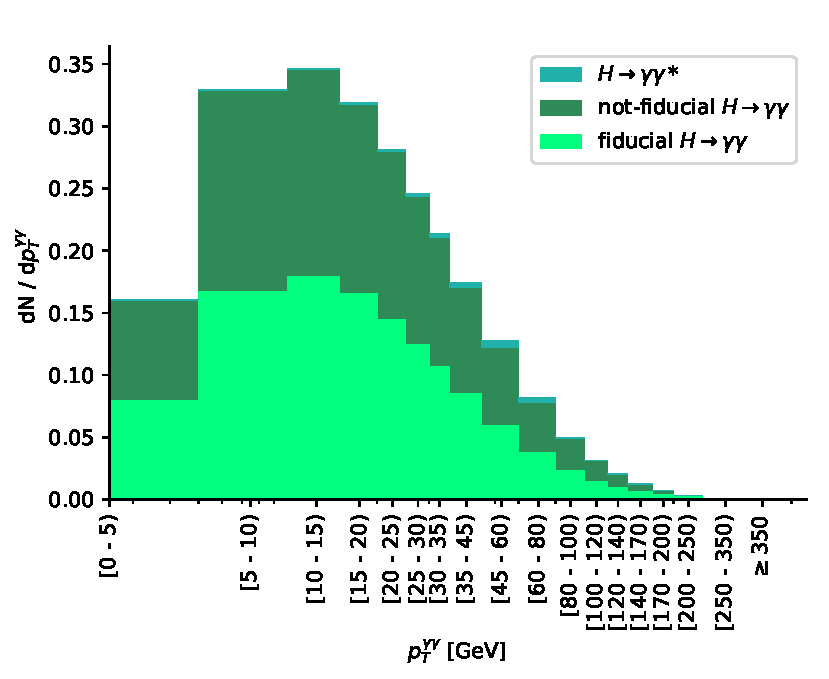
\includegraphics[scale=0.47]{stacked_pT_yy.pdf}}
\subfloat{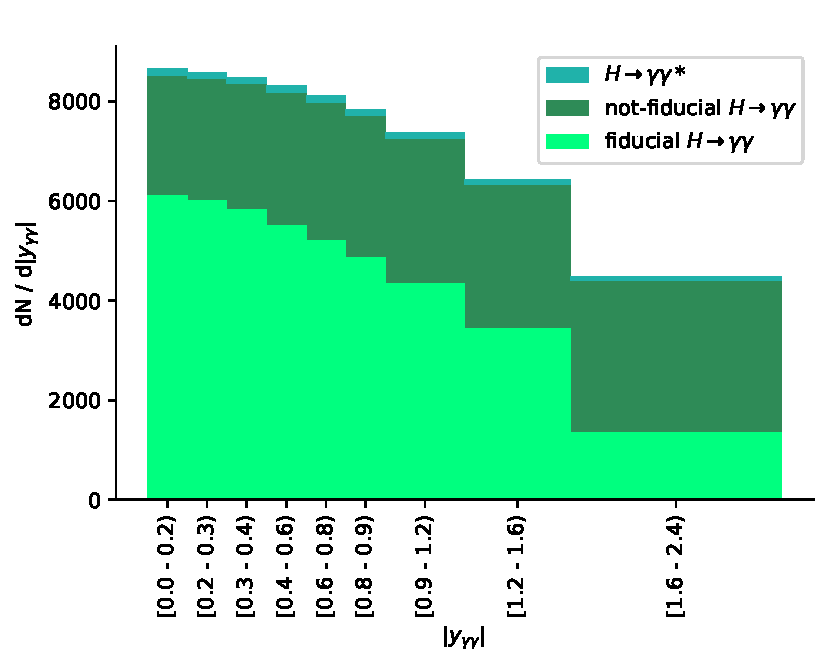
\includegraphics[scale=0.47]{stacked_yAbs_yy.pdf}} 
\end{figure}
\begin{figure}[ht]
\centering
\subfloat{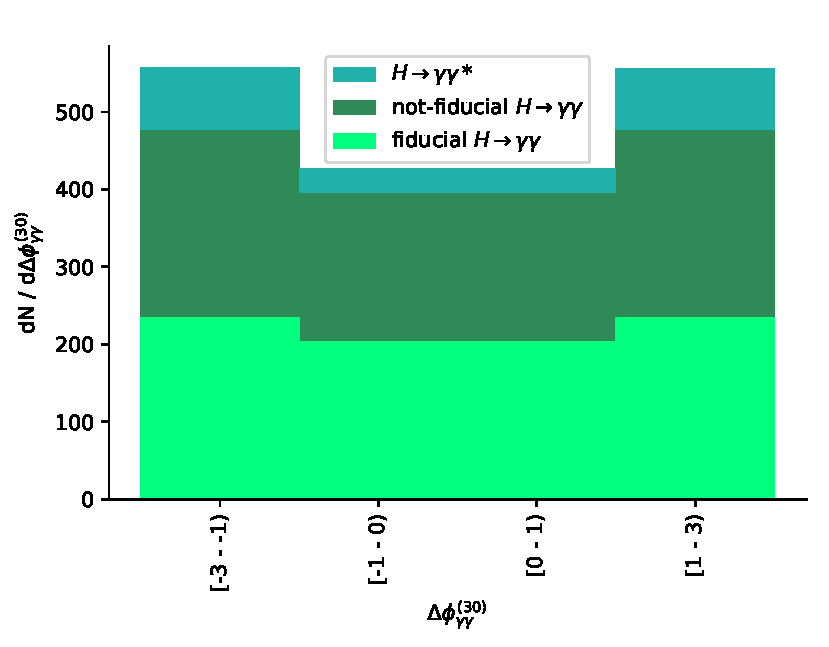
\includegraphics[scale=0.47]{stacked_Dphi_j_j_30_signed.pdf}}
\subfloat{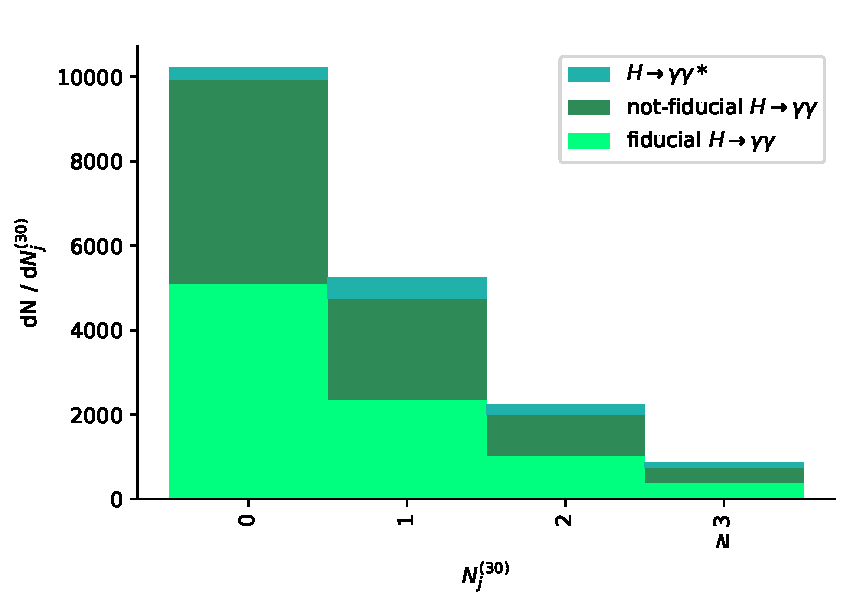
\includegraphics[scale=0.47]{stacked_N_j_30.pdf}} \\
\subfloat{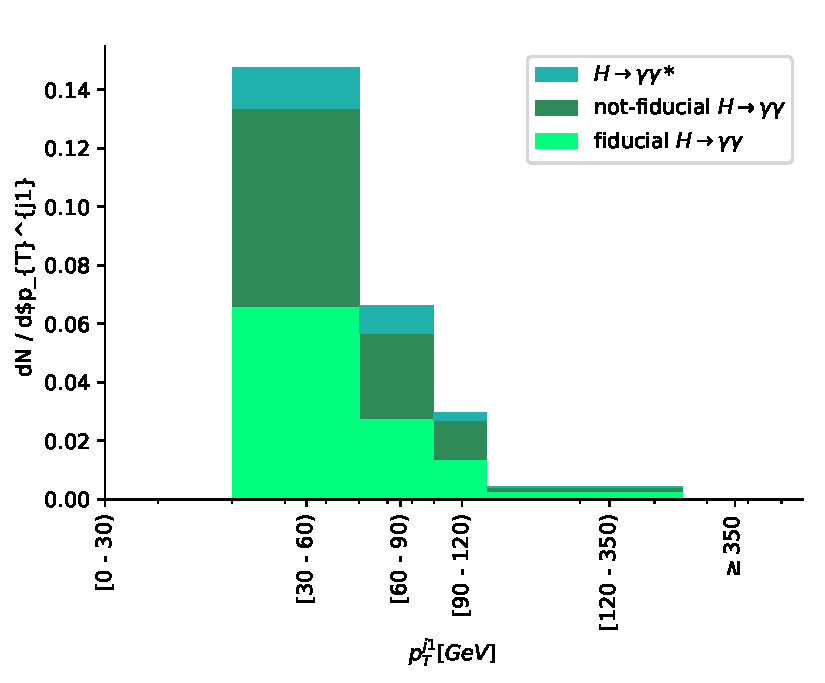
\includegraphics[scale=0.47]{stacked_pT_j1_30.pdf}}
\subfloat{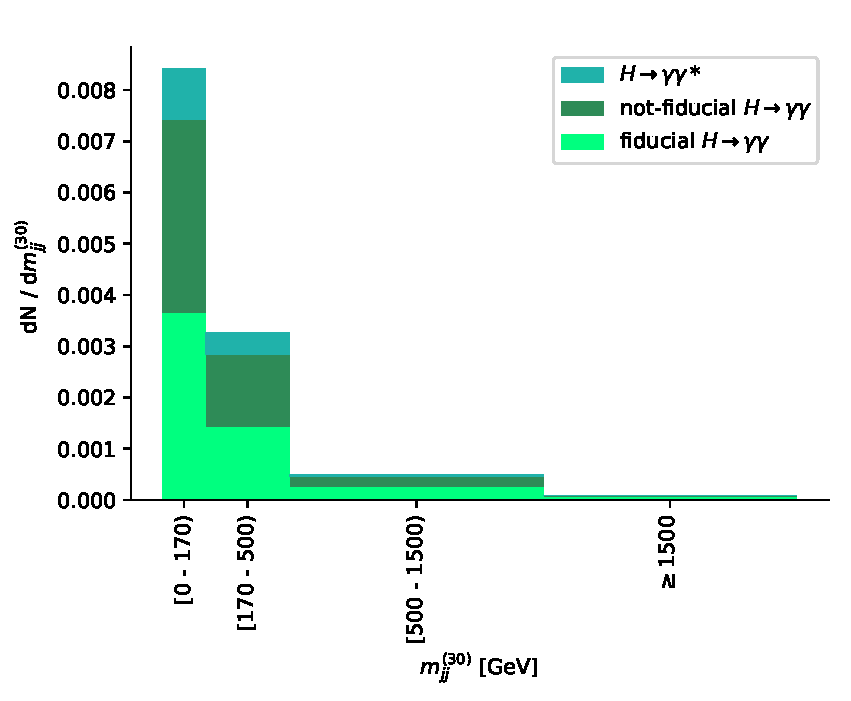
\includegraphics[scale=0.47]{stacked_m_jj_30.pdf}}
\caption{Distribution at true level for all the quantities under investigation. Also the not fiducial events and the Dalitz events are plotted. Notice how the fiducial cuts lower of about $50\%$ the number of events.}
\label{fiducial}
\end{figure}

\section{Event selection}
Collision events are reconstructed in the ATLAS detector by a series of algorithms previously discussed. Objects reconstructed as photons and jets are selected and collected in the analysis dataset.
\begin{itemize}
\item \emph{Photons}: reconstructed from Electromagentic Calorimeter's topo-clusters formed with topological clustering algorithm and classified as converted photons, if there isn't any corresponding track matching in the Inner Detector, or unconverted photons, if corresponding matching tracks are found in the Inner Detector. Reconstructed photons must satisfy $|\eta| < 2.37$ or $1.37 < |\eta| < 1.52$ to fall inside the Electromagnetic Calorimeter barrel or end-cap detecting regions. In order to suppress photons arising from hadrons jets, especially those deriving from $\pi^0 \rightarrow \gamma\gamma$ processes, shower-shape and isolation criteria are imposed, significately optimized for sub-ranges of photon's transverse momentum $p_T$. This $p_T$-dependence in the photons reconstruction and identification brings an efficiency greater than $82\%$ for a photon with $p_T > 25$ GeV. Further calorimeter- and track-based isolation requirements are applied, in order to suppress jets misidentified as photons: the isolation energy $E_T^{\text{iso}}$ is calculated as the transverse energy $E_T$ of the four-momentum sum of all charged particles which have $p_T > 1$ GeV within a cone of $\Delta R  = \sqrt{(\Delta\phi)^2 +(\Delta\eta)^2} < 0.2$ around the photon candidate, subtracting the contribution of the particle candidate and of the underlying and pile-up events. The diphoton system is rejected if the two selected photons do not satisfy $E_T^{\text{iso}} < 0.05 p_T$, while for the calorimeter-based isolation, the system must satisfy $E_T^{\text{iso}} < 0.065 p_T$. Both conditions are intended for each photon candidate of the diphoton system. After the diphoton system selection, the invariant mass of the diphoton system $m_{\gamma\gamma}$ is required to lie in the range $m_{\gamma\gamma} = [105, 160]$ GeV. The leading and sub-leading photons must satisfy the requirement $p_T/m_{\gamma\gamma} > 0.35$ and $p_T/m_{\gamma\gamma} > 0.25$ respectively; 
\\\\
Once the reconstruction process for all photons is performed, the two leading in $pT$ passing the loose identification criteria are selected and chosen as potential $H \rightarrow \gamma\gamma$ decay products. The vertex selection is obtained by using a dedicated neural network, properly trained by simulated ggF $H \rightarrow \gamma\gamma$ events to identify the primary hard interaction vertex in which the Higgs boson is produced. The vertex reconstruction algorithm has around $76\%$ chance of selecting the true Higgs vertex in terms of position resolution, corresponding to a distance uncertainty of $0.03$ mm from the real vertex \cite{ATL-PHYS-PUB-2015-026};

\item \emph{Jets}: reconstructed by clustering calorimeter topological clusters by using the anti-$k_T$ clustering algorithm with a radius parameter of $0.4$. Jets are rejected if they lie within $\Delta R = \sqrt{(\Delta\phi)^2 +(\Delta\eta)^2} < 0.4$ or $\Delta R = \sqrt{(\Delta\phi)^2 +(\Delta\eta)^2} < 0.2$ of a selected photon or selected electron respectively, to avoid the double-counting of the selected particles as jets. In addition, jets are required to have $p_T > 30$ GeV and $|y| < 4.4$, while jets with $|\eta| < 2.5$ and $p_T < 120$ GeV originating from pile-up collisions are suppressed using a jet vertex tagger multivariate discriminant \cite{ATLAS-CONF-2014-018, Aad_2016_pileup}.
\end{itemize}
\section{Signal and background modelling}
The analysis is based on fit of the $m_{\gamma\gamma}$ distribution in various categories, one for each bin to be measured. To do that, a model for the signal and for the background for each category is needed.
\\
Both signal and background modelling are discussed down below. The mass range considered in the analysis is $105 \text{GeV} < m_{\gamma\gamma} < 160 \text{GeV}$, in order to be wide enough to allow the determination of the background continuum from data, made by evaluating the sidebands to both sides of the resonant peak, but not too much to limit the uncertainties from the choice of the background parameterization function.

\subsection{Signal model}
The shape of the $m_{\gamma\gamma}$ for the signal is empirically modeled as a Double-Sided Crystal Ball (CB) function, a  commonly used in High Energy Physics PDF and consisting of a Gaussian core portion and power-law tails on both sided.

\begin{equation}
CB(m_{\gamma\gamma}) = N \times \begin{cases}
									e^{-t^2/2} \hspace{4cm} &\text{if} \hspace{0.2cm} -\alpha_{low} \leq t \leq \alpha_{high} \\
									e^{-\frac{1}{2}\alpha_{low}^2}\Bigl[\frac{1}{R_{low}}(R_{low} - \alpha_{low} - t)\Bigr]^{-n_{low}} \hspace{1cm} &\text{if} \hspace{0.2cm} t < -\alpha_{low} \\
									e^{-\frac{1}{2}\alpha_{high}^2}\Bigl[\frac{1}{R_{high}}(R_{high} - \alpha_{high} - t)\Bigr]^{-n_{high}} \hspace{0.7cm} &\text{if} \hspace{0.2cm} t < -\alpha_{high}
									\end{cases}							
\end{equation}
where
\begin{align}
&t = \frac{m_{\gamma\gamma} - \mu_{CB}}{\sigma_{CB}} \\
&R_{low} = \frac{\alpha_{low}}{n_{low}} \\
&R_{high} = \frac{\alpha_{high}}{n_{high}}
\end{align}
\begin{figure}[htb]
\centering
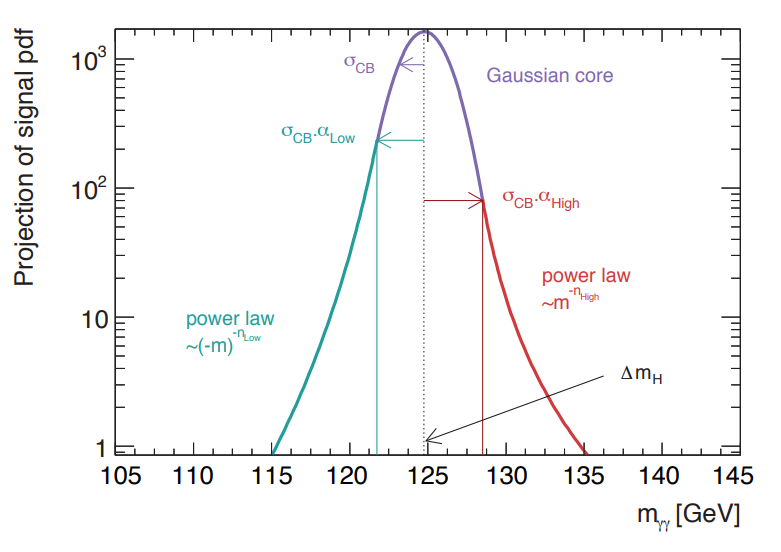
\includegraphics[scale=0.3]{DS_CB.png}
\caption{Example of a Double-Sided Crystal Ball function.}
\label{CB_example}
\end{figure}
and $N$ is the normalization factor, $\mu_{CB}$ is the mean of the Gaussian core distribution, $\sigma_{CB}$ is the width of the Gaussian core distribution, $\alpha_{low/high}$ are the position of the transition from the Gaussian core to the power-law tails on the low and high mass sides respectively and $n_{low/high}$ are the exponents of the low and high mass tails respectively. A detailed description of the procedure is described in \cite{Min_2309522}, while in Figure \ref{CB_example} an example of the Crystal Ball function is presented. 
\\
All the parameters of the Double-Sided Crystal Ball function are obtained by fitting a simulated $H \rightarrow \gamma\gamma$ decays dataset at $m_{\gamma\gamma} = 125$ GeV and then shifting the resonant peak by 90 MeV, in order to optimize the signal model for a Higgs boson with a mass of $125.09$ GeV. Being able to vary for the different bins, the value of each parameter is calculated for each bin of the variable in question. In Figure \ref{signal_param_example} the signal parameterisations for bins with the best and the worst resolution are shown. 
\begin{figure}[htb]
\subfloat[][]{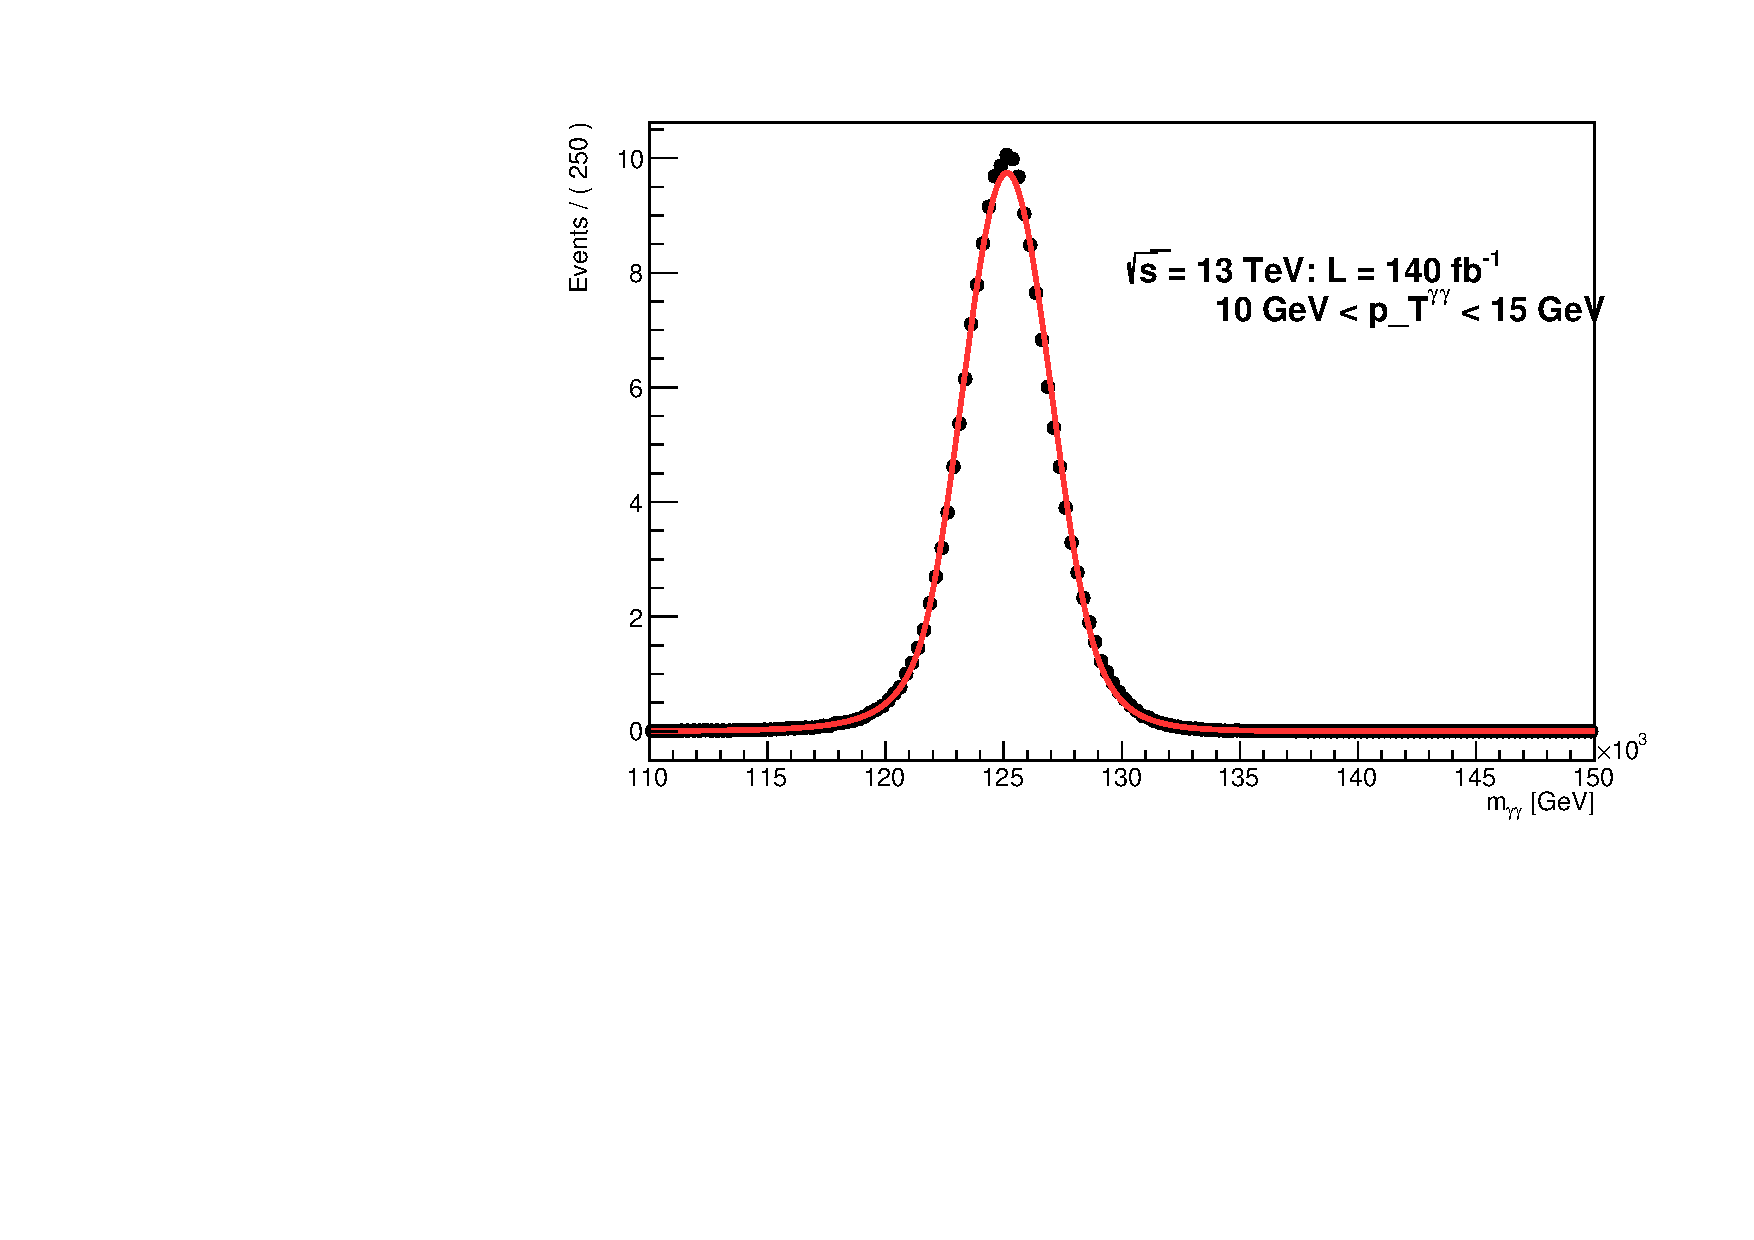
\includegraphics[scale=0.365]{signalParametrisation/fit_pT_yy_bin_3.pdf}}
\subfloat[][]{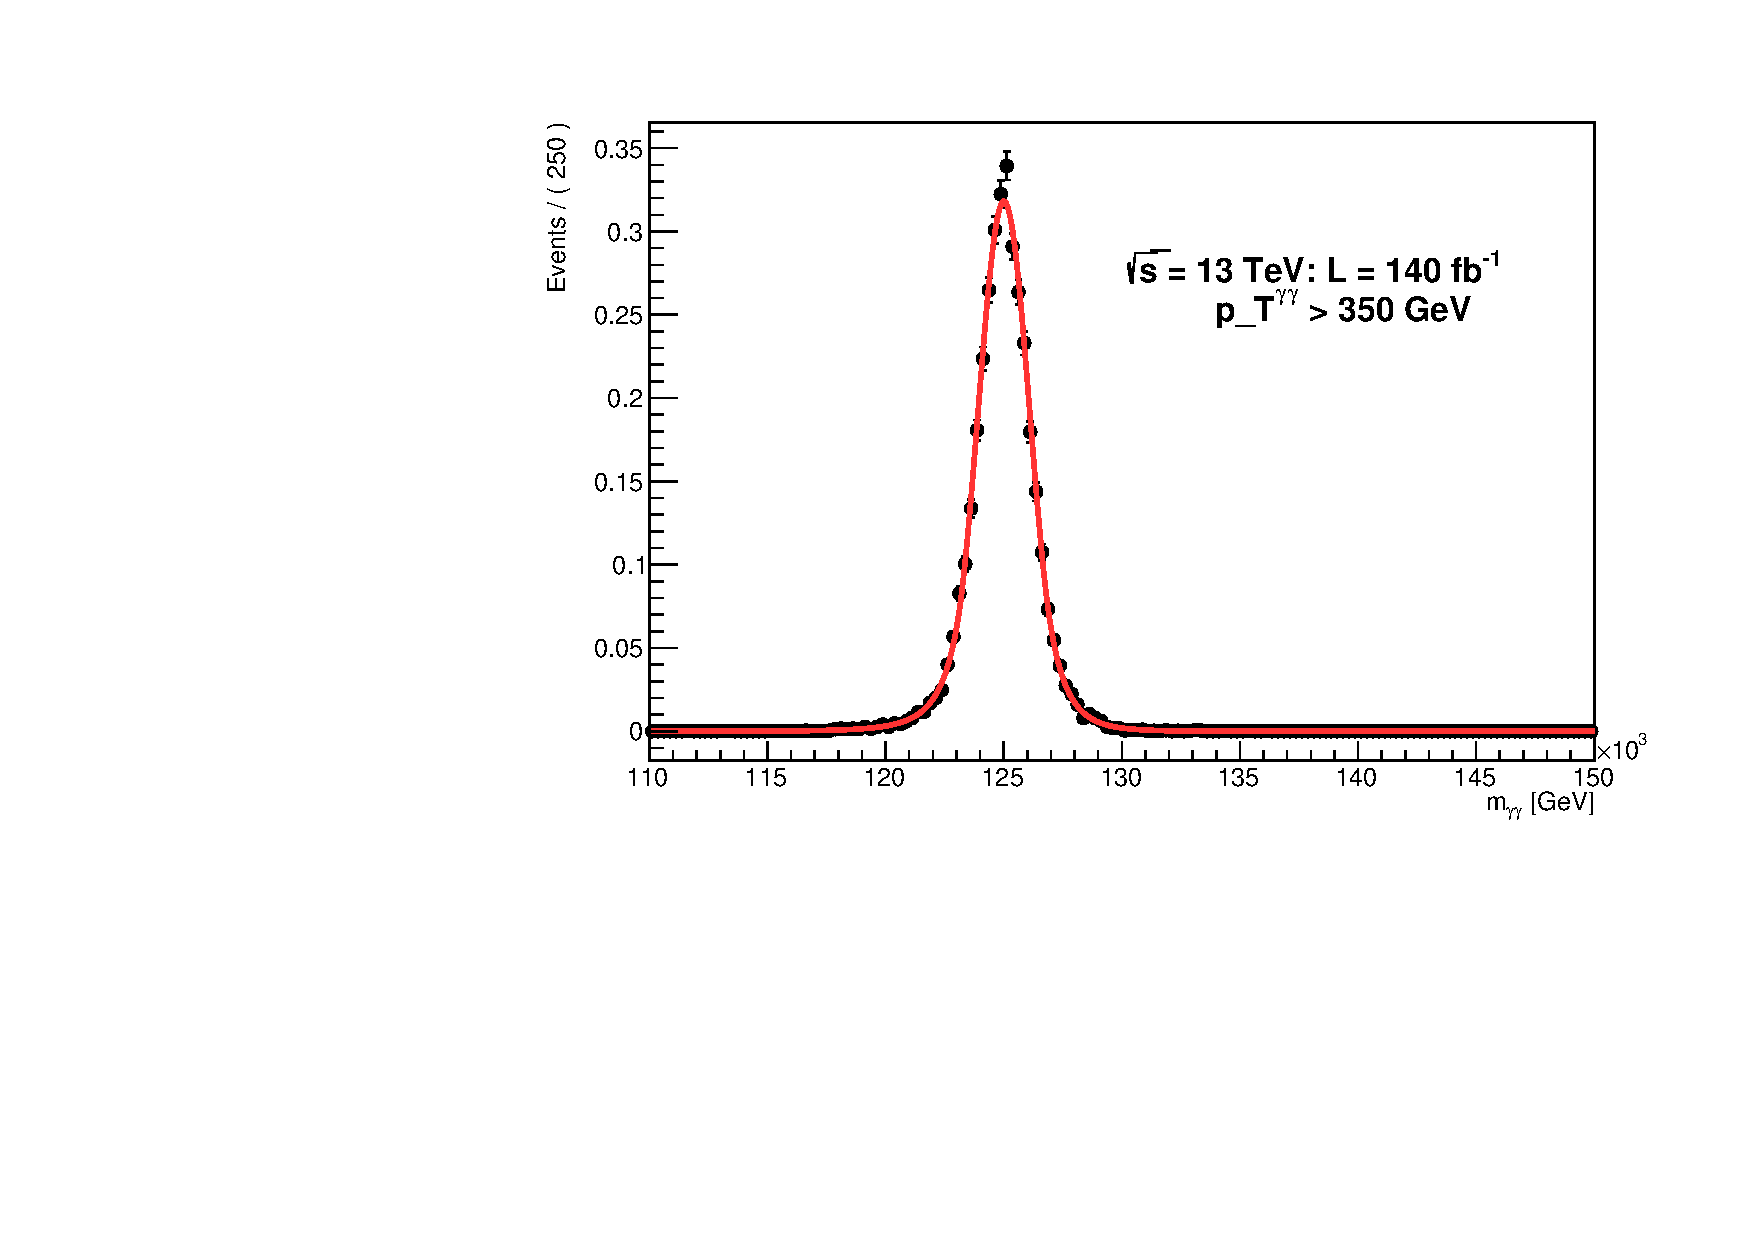
\includegraphics[scale=0.365]{signalParametrisation/fit_pT_yy_bin_18.pdf}}
\caption{a)Signal parameterisation for the fiducial dataset, normalized to $140$ fb$^{-1}$ and to the bin width for bin with the best resolution, b)Signal parameterisation for the fiducial dataset, normalized to $140$ fb$^{-1}$ and to the bin width for bin with the worst resolution. Plots for other observables and bins are shown in Appendix \ref{CB_plots_appendix}.}
\label{signal_param_example}
\end{figure}

\subsection{Background model}
The backgrounds continuum consists of three non resonant components, conforming to the different origin of the photon candidates: the $\gamma\gamma$ component includes selected isolated photons and it is simulated with the S{\scriptsize HERPA} event generator, while the $\gamma j$ and $jj$ components concern the cases where one or both photons candidates in the final state arise from hadronic jets misidentified as photons. The measurement of the background continuum fraction in data is obtained by using a double two-dimensional side-band fitting method for each cross section bin. Being the background distribution an empirically chosen functional form, the shape of the selected function may vary for each bin, incrementing the fit accuracy for each bin and consequently reducing the bias between the fitting function and the data through a spurious signal analysis, further discussed below. An example of background fitting function is shown in Figure \ref{bkg_example}. Several functional forms for the diphoton mass spectrum background are tested: exponentials of first (Exp) and second (ExpPoly$2$) degree polinomials and power law functions of first order (Pow).
\\
The exponential function is defined as 
\begin{equation}
B\Bigl(m_{\gamma\gamma}; \alpha_1^{\text{bkg}}\Bigr) = N\Bigl(\alpha_1^{\text{bkg}}\Bigr) \cdot \text{exp}\Bigl(-\frac{m_{\gamma\gamma}}{\alpha_1^{\text{bkg}}}\Bigr) \hspace{0.2cm} \text{,}
\end{equation}
while the second order exponential polynomial is defined as
\begin{equation}
B\Bigl(m_{\gamma\gamma}; \alpha_1^{\text{bkg}}, \alpha_2^{\text{bkg}}\Bigr) = N\Bigl(\alpha_1^{\text{bkg}}, \alpha_2^{\text{bkg}}\Bigr) \cdot \text{exp}\Bigl(-\frac{m_{\gamma\gamma}}{\alpha_1^{\text{bkg}}} - \frac{m_{\gamma\gamma}^2}{\alpha_2^{\text{bkg}}}\Bigr) \hspace{0.2cm} \text{,}
\end{equation}
where $\alpha_i^{\text{bkg}}$ are nuisance parameters and $N($\textbf{$\alpha^{\text{bkg}}$}$)$ is a normalization factor. In general, a higher-order exponential is preferred for bins with more events.
\\
Lastly, the first order power-law function is defined as
\begin{equation}
B\Bigl(m_{\gamma\gamma}; \alpha_1^{\text{bkg}}\Bigr) = N\Bigl(\alpha_1^{\text{bkg}}\Bigr) \cdot (m_{\gamma\gamma})^{\alpha^1}
\end{equation}
The choice of the background functional form is performed to minimize the bias due to potential mismodelling.
\begin{figure}[hbt]
\centering
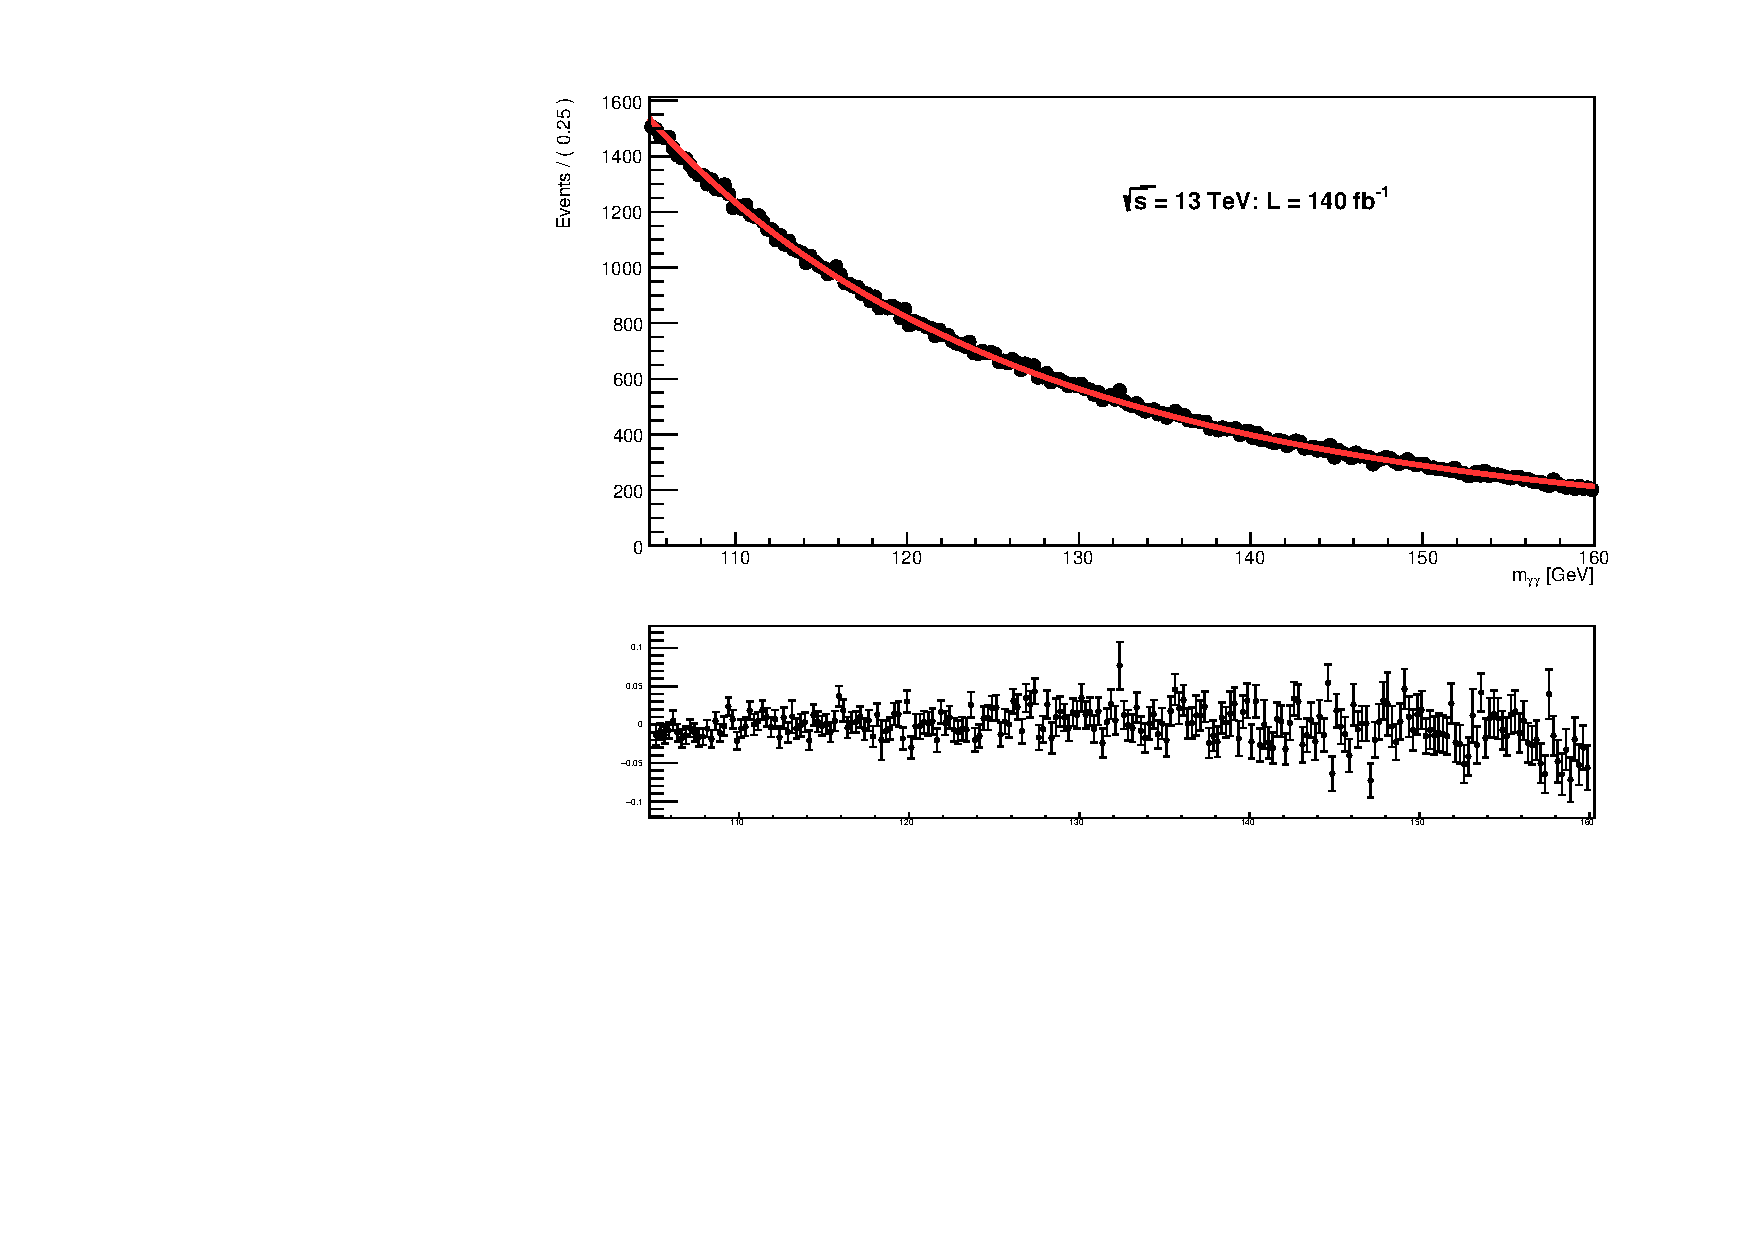
\includegraphics[scale=0.46]{fitPlot_pT_yy_bin_3_pow.pdf}
\caption{Example of fitting process for the background dataset in the mass range $105 \text{GeV} < m_{\gamma\gamma} < 160 \text{GeV}$ performed using the parametrization function with the minimum spurious signal (Pow) in the $pT_{\gamma\gamma}$ bin with best resolution ($10 \text{GeV} < p_T^{\gamma\gamma} < 15 \text{GeV}$).}
\label{bkg_example}
\end{figure}

\subsection{Spurious signal}
\label{spur_sign_sec}
The spurious signal method is used to study the bias in the signal yield evaluation for each observable bin. This kind of analysis is performed by fitting a background-only MonteCarlo sample with a distribution including both signal and background. The background sample is made mixing the $\gamma\gamma$, $\gamma j$ components following a data-driven approach. The $\gamma\gamma$ component is derived from S{\scriptsize HERPA} MonteCarlo simulation, while the $\gamma j$ component is taken from a control region. The $jj$ component is ignored in the background composition since it is negligible respect to the others. In principle, a null signal yield is expected from the fit. The effective yield of the fitted signal si called \emph{Spurious Signal} $SS$.
\\
The spurious signal yield extracted in this way from the background-only template $SS$ and its statistical uncertainty $\Delta_{SS}$ are used in the background parameterisation functions selection.
\begin{figure}[b!]
\centering
\subfloat{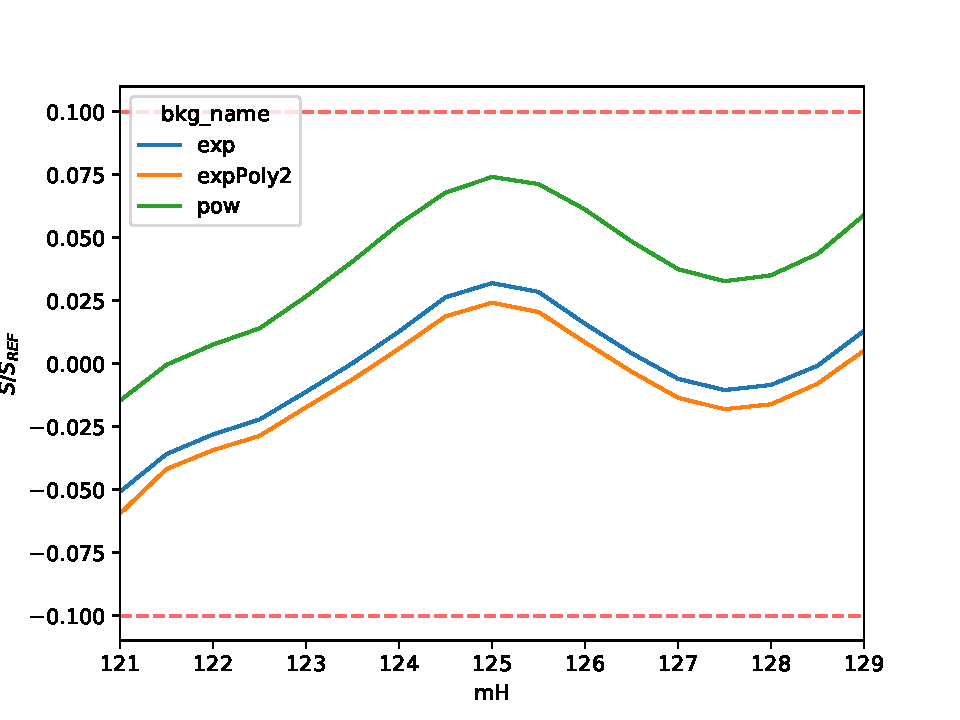
\includegraphics[scale=0.38]{total_Mu_pT_yy_bin_16.pdf}}
\subfloat{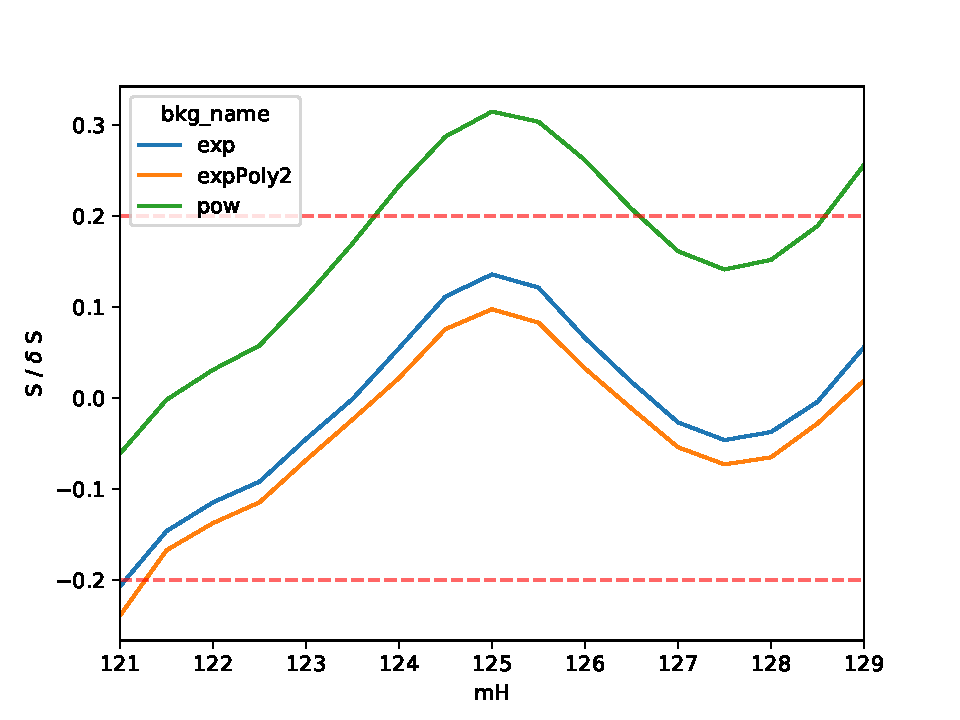
\includegraphics[scale=0.38]{total_Z_pT_yy_bin_16.pdf}} \\
\subfloat{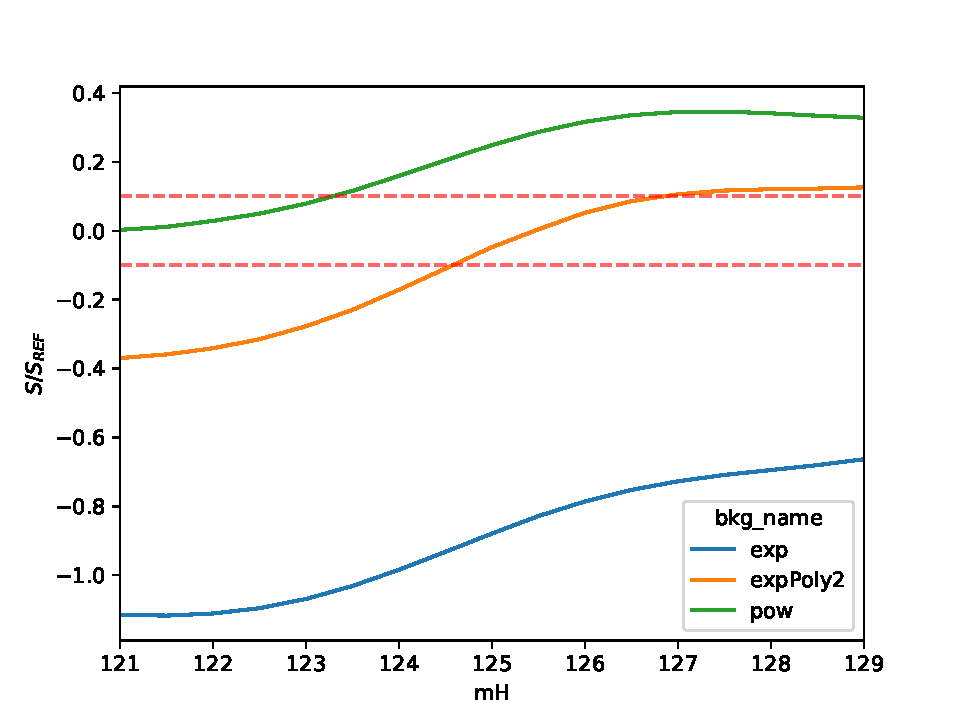
\includegraphics[scale=0.38]{total_Mu_pT_yy_bin_3.pdf}}
\subfloat{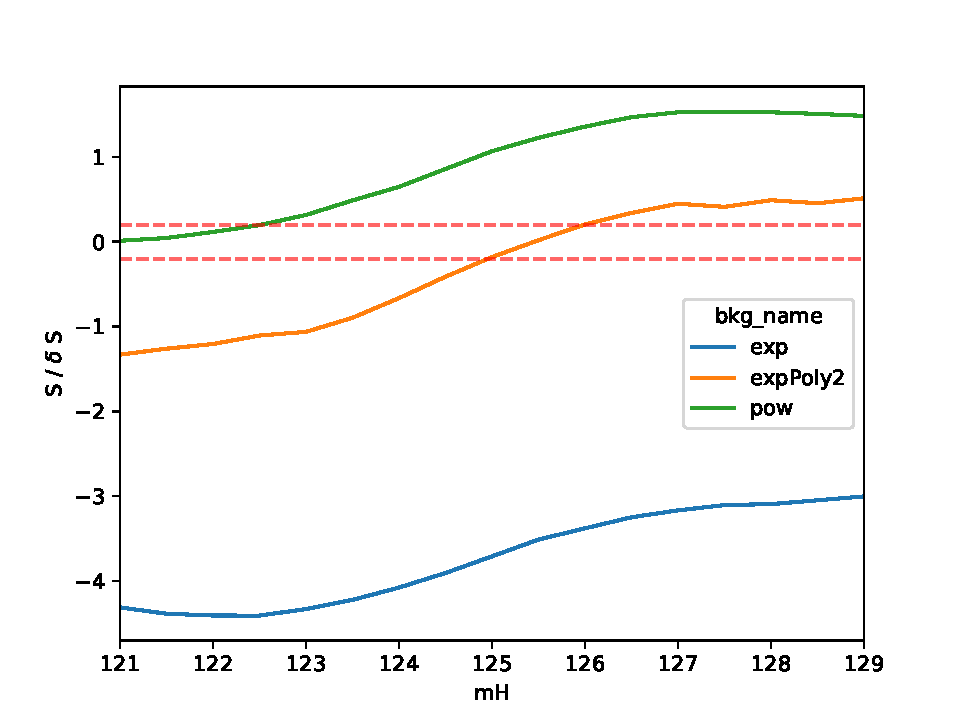
\includegraphics[scale=0.38]{total_Z_pT_yy_bin_3.pdf}} \\
\caption{Plots of $SS/S_{ref}$ and $SS/\Delta SS$ for $p_T^{\gamma\gamma}$ distribution in the best (upper plots for bin $16$) and worst (lower plots for bin $3$) bins. The dashed red lines show the selection conditions under which a functional form is selected ora rejected.}
\label{SS_example}
\end{figure}
\\The condition (Figure \ref{SS_example}) for a functional form to be accepted is that either
\begin{itemize}
\item $SS < 20 \%$ of the background uncertainty;
\item $SS < 10 \%$ of the number of expected signal events.
\end{itemize}
\begin{table}[h]
\centering
\small
\caption{Background templates and spurious signal results for the individual bins in $p_T^{\gamma\gamma}$ distribution.}
\label{SS}
\begin{tabular}{c | c | l r r r}
Bin & Range & Function & $|Max(SS)|$ & $SS/S_{ref} [\%]$ & $SS/\Delta SS [\%]$ \\
\hline
1 & $0 \text{GeV} < p_T^{\gamma\gamma} < 5 \text{GeV}$ & Pow & 37.4 & 13.6 & 38.4 \\
2 & $5 \text{GeV} < p_T^{\gamma\gamma} < 10 \text{GeV}$ & ExpPoly2 & 88.9 & 15.1 & 59.7 \\
3 & $10 \text{GeV} < p_T^{\gamma\gamma} < 15 \text{GeV}$ & Pow & 219.3 & 34.6 & 153.0 \\
4 & $15 \text{GeV} < p_T^{\gamma\gamma} < 20 \text{GeV}$ & ExpPoly2 & 67.5 & 11.6 & 40.3 \\
5 & $20 \text{GeV} < p_T^{\gamma\gamma} < 25 \text{GeV}$ & ExpPoly2 & 120.1 & 23.5 & 73.5 \\
6 & $25 \text{GeV} < p_T^{\gamma\gamma} < 30 \text{GeV}$ & ExpPoly2 & 25.9 & 5.9 & 20.6 \\
7 & $30 \text{GeV} < p_T^{\gamma\gamma} < 35 \text{GeV}$ & ExpPoly2 & 71.1 & 18.9 & 57.2 \\
8 & $35 \text{GeV} < p_T^{\gamma\gamma} < 45 \text{GeV}$ & ExpPoly2 & 61.6 & 10.3 & 38.6 \\
9 & $45 \text{GeV} < p_T^{\gamma\gamma} < 60 \text{GeV}$ & ExpPoly2 & 82.1 & 13.1 & 59.7 \\
10 & $60 \text{GeV} < p_T^{\gamma\gamma} < 80 \text{GeV}$ & Exp & 27.6 & 5.3 & 21.6 \\
11 & $80 \text{GeV} < p_T^{\gamma\gamma} < 100 \text{GeV}$ & ExpPoly2 & 59.1 & 18.2 & 62.8 \\
12 & $100 \text{GeV} < p_T^{\gamma\gamma} < 120 \text{GeV}$ & ExpPoly2 & 47.6 & 22.7 & 74.2 \\
13 & $120 \text{GeV} < p_T^{\gamma\gamma} < 140 \text{GeV}$ & ExpPoly2 & 13.1 & 9.0 & 29.3 \\
14 & $140 \text{GeV} < p_T^{\gamma\gamma} < 170 \text{GeV}$ & Pow & 23.3 & 16.1 & 64.1 \\
15 & $170 \text{GeV} < p_T^{\gamma\gamma} < 200 \text{GeV}$ & Pow & 15.3 & 17.3 & 65.9 \\
16 & $200 \text{GeV} < p_T^{\gamma\gamma} < 250 \text{GeV}$ & Exp & 4.0 & 5.0 & 20.4 \\
17 & $250 \text{GeV} < p_T^{\gamma\gamma} < 350 \text{GeV}$ & Pow & 4.5 & 8.0 & 33.3 \\
18 & $p_T^{\gamma\gamma} \geq 350 \text{GeV}$ & Pow & 5.8 & 26.1 & 93.5
\end{tabular}
\end{table}
In the case of none of the functions is selected, the selection criteria is based on the choice of the functional form which has the minimum value for the spurious signal, in order to find the function which best describes the background spectrum.
\\
In Table \ref{SS} the selected best background parameterisations for $p_T^{\gamma\gamma}$ distribution and relative spurious signals are summarized . The selected background functions for other observables are presented in Appendix \ref{CB_parameters_appendix}.
\\
For each bin of the observable's distribution, the selected function is given, followed by the maximal spurious signal value $|Max(SS)|$ and the spurious signal uncertainty $SS/S_{ref}$ for that function in the single bin. The spurious signal uncertainty is evaluated as the ratio between the maximal spurious signal value and the reference signal based on MonteCarlo simulations.

\section{Unfolding}
In any experimental analysis, the distribution of every observable is distorted and biased due to experimental limitations effects, as the limited acceptance, the reconstruction efficiency and the finite resolution. The unfolding is the procedure to correct a measured quantity estimating the \emph{truth-level} spectrum, once the \emph{reco-level} distribution is known.
\\
Through the unfolding procedure it is possible to obtain results independent of detector and reconstruction effects, making in this way the unfolded differential distributions easily comparable among different experiments and with the theoretical predictions too \cite{refId0}.
\\\\
In this work, two different unfolding methods are tested, in order to obtain the best corrections to be applied at the measured differential cross sections, so they can be unfolded to particle level cross sections and in this way compared to the theoretical Standard Model predictions:
\begin{itemize}
\item the \emph{bin-by-bin} unfolding method;
\item the \emph{inverse-matrix} unfolding method.
\end{itemize}
The theoretical predictions used are the ones provided by the MonteCarlo simulations described in Section \ref{mc_sim}.

\subsection{The bin-by-bin unfolding method}
\label{c_factors_sec}
The bin-by-bin method corrects the reconstructed events with the true number of events (Figure \ref{true/reco}) with just a multiplicative factor for each bin, called \emph{c factor}.
\\
Consider $N_i^{\text{reco, peak}}$ as the expected reconstructed signal yield under the resonant peak (e.g. the Crystal Ball function) in a given reconstructed category. This quantity can be derived from the expected signal yield at particle level in the corresponding fiducial bin $N_i^\text{true, $\gamma\gamma$, fid}$ through the relation
\begin{equation}
N^\text{reco, peak}_i = \underbrace{L \sigma_i^\text{fid} Br_{\gamma\gamma}}_{N_i^\text{true, $\gamma\gamma$, fid}} \cdot C_i
\end{equation}
simply scaling $N_i^{\text{true, }\gamma\gamma \text{, fid}}$, the number of signal events at particle level in the fiducial region, by the correction factor $C_i$, shown for each distribution in Table \ref{c_factors_table}. These factors are computed from MonteCarlo simulations as the ratio of the number of signal events expected to pass the detector level criteria and the number of events expected to pass the corresponding particle level criteria
\begin{equation}
C_i = \left(\frac{N^\text{reco, peak}_i}{N_i^\text{true, $\gamma\gamma$, fid}}\right)_\text{MC}
\end{equation}
where the number of expected events at both detector reconstructed and particle level are computed from MonteCarlo simulations considering all the production modes.
\begin{figure}[b!]
\centering
\includegraphics[scale=0.6]{reco-true_comparison/comparison_true_reco_pT_yy_for_c_factors.pdf}
\caption{Comparison of the $p_T^{\gamma\gamma}$ distribution at reco level for events passing the particle level criteria and for events passing the corresponding detector reconstructed level criteria, computed by using MonteCarlo simulation.}
\label{true/reco}
\end{figure}
\begin{table}[h]
\centering
\small
\caption{Bin-by-bin correction factors for each bin of all observables' distributions.}
\label{c_factors_table}
\begin{tabular}{l | rrrrrr}
Bin &  $p_T^{\gamma\gamma}$ & $|y|_{\gamma\gamma}$ & $p_T^{j1, 30}$ & $\Delta\phi_{jj}^{30}$ & $N_j^{30}$ & $m_{jj}^{30}$ \\
\hline
0 &					- & 				- & 				0.64 & 					0.68 & 			- & 			0.68 \\ 
1 &                  0.69 &                 0.72 &           0.84 &                   0.82 &       0.65 &          0.87 \\
2  &                  0.71 &                 0.72 &           0.71 &                   0.86 &       0.76 &           0.8 \\
3  &                  0.71 &                 0.72 &           0.72 &                   0.86 &        0.8 &          0.85 \\
4  &                  0.71 &                 0.72 &           0.75 &                   0.82 &       0.95 &           0.9 \\
5  &                  0.71 &                 0.72 &           0.77 &                      - &          - &             - \\
6  &                  0.71 &                 0.72 &           0.76 &                      - &          - &             - \\
7  &                  0.70 &                  0.70 &              - &                      - &          - &             - \\
8  &                  0.70 &                 0.69 &              - &                      - &          - &             - \\
9  &                  0.70 &                 0.68 &              - &                      - &          - &             - \\
10 &                  0.70 &                    - &              - &                      - &          - &             - \\
11 &                  0.70 &                    - &              - &                      - &          - &             - \\
12 &                  0.72 &                    - &              - &                      - &          - &             - \\
13 &                  0.73 &                    - &              - &                      - &          - &             - \\
14 &                  0.75 &                    - &              - &                      - &          - &             - \\
15 &                  0.76 &                    - &              - &                      - &          - &             - \\
16 &                  0.77 &                    - &              - &                      - &          - &             - \\
17 &                  0.79 &                    - &              - &                      - &          - &             - \\
18 &                  0.80 &                    - &              - &                      - &          - &             - 
\end{tabular}
\end{table}
\\The $N^\text{reco, peak}_i$ expected yields must take into account both $H \rightarrow \gamma\gamma$ (fiducial and not fiducial) and the $H \rightarrow \gamma\gamma *$ resonant processes, the latter generally known as Dalitz processes, which cannot be distinguished at detector reconstructed level, while $N^\text{true, $\gamma\gamma$, fid}_i$ is computed only for $H \rightarrow \gamma\gamma$
\begin{align}
N^\text{reco, peak}_i &= N^\text{reco, peak, $\gamma\gamma$}_i + N^\text{reco, peak, $\gamma\gamma^*$}_i \\
&= \sum_{S\in\text{samples}} L_S \sigma_S Br_{\gamma\gamma} P(\text{pass}, i|S, \gamma\gamma) + (\gamma\gamma\leftrightarrow\gamma\gamma^*) \\
&= \sum_{S\in\text{samples}} L_S \sigma_S Br_{\gamma\gamma} \left(\frac{ \sum_{n\in\text{pass, i, $\gamma\gamma$}} w^\text{final}_{n} } { \sum_{n\in\gamma\gamma} w^\text{initial}_{n} }\right)_S + (\gamma\gamma\leftrightarrow\gamma\gamma^*)
\end{align}
\begin{align}
N^\text{true, $\gamma\gamma$, fid}_i
&= \sum_{S\in\text{samples}} L_S \sigma_S Br_{\gamma\gamma} \underbrace{P(\text{true-fid-$i$}|S, \gamma\gamma)}_{A_{S, i}}\\
&= \sum_{S\in\text{samples}} L_S \sigma_S Br_{\gamma\gamma} \left(\frac{ \sum_{n\in\text{i, $\gamma\gamma$}} w^\text{initial}_{n} } { \sum_{n\in\gamma\gamma} w^\text{initial}_{n} }\right)_S
\end{align}
where the $P(\text{pass}, i|S, \gamma\gamma)$ is the probability for a reconstructed event to pass the selection criteria, computed as the the ratio between the number of events passing the selection and the total number of events at particle level for a given sample, while $P(\text{true-fid-$i$}|S, \gamma\gamma)$, generally known as the acceptance $A_{S, i}$, is the probability for a particle level event to fall in the fiducial phase space for a given sample. The summations are done over all the samples, for each production mode and different period.

\subsection{The inverse-matrix unfolding method}
\label{matrix_sec}
Differently from the bin-by-bin unfolding method, in the inverse matrix unfolding method the migrations and correlations between bins in the detector reconstruction are explicitely modelled. The matrix considered here is the signal efficiency matrix which describes both the efficiency and the migration effects \cite{article_matrix_method}. Some care should be taken to take into account resonant events which are not signal: Dalitz $H \rightarrow \gamma\gamma *$ and out of fiducial $H \rightarrow \gamma\gamma$ events.
\\\\
In case of infinite detector resolution and no other biasing effects, the detector response matrix is just a diagonal matrix, where for each reconstructed bin is associated only the corresponding bin at particle level. In a normal experiment, though, experimental limitation effects leads to events' migrations passing from particle level to the detector reconstructed ones, corrected by the coefficients turning out from the inverse detector response matrix.
\\\\
Considering the number of expected selected events under the resonant peak $N^\text{reco, peak}_R$, in the detector reconstructed category $R$, it can be decomposed in the two components for the $H \rightarrow \gamma\gamma$ and $H \rightarrow \gamma\gamma *$ processes
\begin{align}
N^\text{reco, peak}_R &= N^\text{reco, peak, $\gamma\gamma$}_R + N^\text{reco, peak, $\gamma\gamma^*$}_R \\
&= \sum_{T\neq \gamma\gamma^*} N^\text{reco, peak}_{R,T} + N^\text{reco, peak}_{R, \gamma\gamma^*} \\
&= \sum_{T\neq \gamma\gamma^*} N_{T}\mathlarger{\varepsilon}(R|T) + N_{T=\gamma\gamma*}\mathlarger{\varepsilon}(R|\gamma\gamma^*) \\
&= \sum_{T\neq \gamma\gamma^*} L \sigma_T Br_{\gamma\gamma} \mathlarger{\varepsilon}(R|T) + L\underbrace{\left(\sum_{T\neq\gamma\gamma*}\sigma_\text{T}\right)}_{\sigma^\text{tot}} Br_{\gamma\gamma^*} \mathlarger{\varepsilon}(R|\gamma\gamma^*)
\end{align}
\phantom{i}\hspace{0.5cm}$R = $ (reco pass bin1), (reco pass bin2), \ldots,
\\
\phantom{i}\hspace{0.5cm}$T = $ ($\gamma\gamma$ fiducial bin1), ($\gamma\gamma$ fiducial bin2), \ldots, ($\gamma\gamma$ not-fiducial), ($\underbrace{\gamma\gamma^*}_\text{Dalitz}$)
\\
where $N^\text{reco, peak}_R$ are the expected number of events reconstructed in bin $R$ coming from the bin $T$, while $N_T$ is the number of events generated in the true bin $T$.
\\\\
The efficiency matrix $\mathlarger{\varepsilon}(R|T)$, generally known as \emph{folding matrix} and deriving from the yield matrix in Figure \ref{yield_matrix}, is evaluated from MonteCarlo simulations and represents the probability for a given particle-level $T$ event to be reconstructed as a given detector reconstructed $R$ event
\begin{equation}
\mathlarger{\varepsilon}(R|T) = P[R|T] = \left(\frac{N_{R, T}}{N_T}\right)_\text{MC}
\end{equation}
In the case of Dalitz $H \rightarrow \gamma\gamma *$ events, the Branching Ratio $Br_{\gamma\gamma^*}$ is derived from the $H \rightarrow \gamma\gamma$ Branching Ratio $Br_{\gamma\gamma}$, rescaled by the fraction of Dalitz events in the MonteCarlo dataset
\begin{equation}
Br_{\gamma\gamma*} = Br_{\gamma\gamma}\times\left( \frac{N_{\gamma\gamma^*}}{N_{\gamma\gamma}}\right)_\text{MC}
\end{equation}
while the out of fiducial cross sections $\sigma_\text{$\gamma\gamma$, not-fiducial}$, being those impossible to be reconstructed at detector level due to the finite detecting acceptance, are taken rescaling the total cross section $\sigma_\text{tot}$ by the acceptance of the detector $A_\text{not-fiducial}$
\begin{equation}
\sigma_\text{$\gamma\gamma$, not-fiducial} = \sigma^\text{tot} \times A_\text{not-fiducial} =\underbrace{\left(\sum_{T\neq\gamma\gamma^*, \text{non-fid}}\sigma_T\right)}_{\sigma^\text{fid}}\times\frac{A_\text{not-fiducial}}{1-A_\text{not-fiducial}}
\end{equation}
with
\begin{equation}
A_\text{not-fiducial}=\left(\frac{N_\text{$\gamma\gamma$, not-fiducial}}{N_{\gamma\gamma}}\right)_\text{MC}
\end{equation}
With respect to the analysis published by ATLAS \cite{ATLAS-CONF-2018-018}, the different and original approach of this work consists in considering the Dalitz and the out of fiducial phase space events in separate and distinct categories, in order to improve the accuracy of the unfolding method.
\\
As an example, in Figure \ref{pT_yy_migration} the migration matrix for $p_T^{\gamma\gamma}$ distribution is shown. It can be seen how, as growing values of $p_T^{\gamma\gamma}$, the migration contributions get smaller due to improving of the detector resolution. In the first two rows the separated Dalitz and out of fiducial phase space categories are displayed. Thanks to the design of the selection cut, the contribution from non-fiducial region and Dalitz events is very small.
\begin{figure}[H]
\centering
\subfloat[][]{\includegraphics[scale=0.44]{folding_matrices/yield_reco_true_All_pT_yy_mcAll_prodAll_sysNominal_LUMI_138972.pdf}
\label{yield_matrix}} \\
\subfloat[][]{\includegraphics[scale=0.44]{folding_matrices/folding_matrix_P_reco_true_All_pT_yy_mcAll_prodAll_sysNominal_LUMI_138972.pdf}
\label{pT_yy_migration}}
\caption{a)Expected yield for each reconstructed and true bin, normalized to $140$ fb$^{-1}$; b)Migration matrix for $p_T^{\gamma\gamma}$ distribution using the dataset normalized to $140$ fb$^{-1}$. The notPassed bins are not used in the analysis.}
\end{figure}

\section{Statistical model}
The fiducial differential cross sections are extracted performing a simultaneous fit on the  $m_{\gamma\gamma}$ distribution over every bin of each observable. A PDF combines the signal Double-Sided Crystal Ball parameterisation and the background for the considered bin. The observed values are derived fitting data, while the expected ones are obtained through a fit from Asimov dataset. The likelihood function is defined as in Eq.(\ref{likelihood})
\begin{equation}
\mathcal{L}_R(m_{\gamma\gamma}; \vec{\sigma}, N_{\text{bkg}}, \vec{\theta}) = \frac{e^{-\nu}}{n!} \prod_{j}^{n}\Bigl[N_R^{\text{Reco, peak}}(\vec{\sigma}, \vec{\theta}) \mathcal{S}(m_{\gamma\gamma}^j; \vec{\theta}) + N_{\text{bkg}, R} \mathcal{B}_R(m_{\gamma\gamma}^j)\Bigr]
\label{likelihood}
\end{equation} 
\begin{table}[h]
\centering
\tiny
\caption{Energy scale systematics $\sigma_{ES}$ on the left and energy resolution systematics on the right, expressed in \%, for each observable in the analysis.}
\label{ES_ER_table}
\begin{tabular}{l | cccccc}
Bin & $p_T^{\gamma\gamma}$ & $|y|_{\gamma\gamma}$ & $p_T^{j1}$ & $\Delta\phi_{jj}^{30}$ & $N_j^{30}$ & $m_{jj}^{30}$ \\
\hline
0 & - & - & 0.43 & 0.43 & - & 0.43 \\
1 & 0.42 & 0.27 & 0.44 & 0.46 & 0.43 & 0.48 \\
2 & 0.42 & 0.28 & 0.47 & 0.51 & 0.45 & 0.49 \\
3 & 0.42 & 0.30 & 0.49 & 0.51 & 0.48 & 0.49 \\
4 & 0.42 & 0.34 & 0.54 & 0.46 & 0.51 & 0.50 \\
5 & 0.42 & 0.38 & 0.54 & - & - & - \\
6 & 0.42 & 0.44 & 0.63 & - & - & - \\
7 & 0.43 & 0.53 & - & - & - & - \\
8 & 0.43 & 0.60 & - & - & - & - \\
9 & 0.44 & 0.66 & - & - & - & - \\
10 & 0.46 & - & - & - & - & - \\
11 & 0.47 & - & - & - & - & - \\
12 & 0.48 & - & - & - & - & - \\
13 & 0.50 & - & - & - & - & - \\
14 & 0.53 & - & - & - & - & - \\
15 & 0.55 & - & - & - & - & - \\
16 & 0.58 & - & - & - & - & - \\
17 & 0.62 & - & - & - & - & - \\
18 & 0.65 & - & - & - & - & - \\
\end{tabular} \qquad
\begin{tabular}{l | cccccc}
Bin & $p_T^{\gamma\gamma}$ & $|y|_{\gamma\gamma}$ & $p_T^{j1}$ & $\Delta\phi_{jj}^{30}$ & $N_j^{30}$ & $m_{jj}^{30}$ \\
\hline
0 & - & - & 6.8 & 7.0 & - & 7.0 \\ 
1 & 6.6 & 5.4 & 7.2 & 7.8 & 6.8 & 8.4 \\
2 & 6.5 & 5.4 & 7.8 & 9.2 & 7.5 & 8.6 \\
3 & 6.5 & 5.6 & 8.6 & 9.4 & 8.3 & 8.9 \\
4 & 6.5 & 5.8 & 10.7 & 8.0 & 9.1 & 8.3 \\
5 & 6.5 & 6.1 & 10.7 & - & - & - \\
6 & 6.6 & 6.5 & 16.5 & - & - & - \\
7 & 6.7 & 7.0 & - & - & - & - \\
8 & 6.9 & 8.4 & - & - & - & - \\
9 & 7.0 & 10.8 & - & - & - & - \\
10 & 7.1 & - & - & - & - & - \\
11 & 7.7 & - & - & - & - & - \\
12 & 7.9 & - & - & - & - & - \\
13 & 8.4 & - & - & - & - & - \\
14 & 10.6 & - & - & - & - & - \\
15 & 11.1 & - & - & - & - & - \\
16 & 12.4 & - & - & - & - & - \\
17 & 14.5 & - & - & - & - & - \\
18 & 18.0 & - & - & - & - & - \\
\end{tabular}
\end{table}
\\In Eq.(\ref{likelihood}) many ingredients are recognisable: $m_{\gamma\gamma}^j$ is the diphoton invariant mass for the event $j$, $\mathcal{S}(m_{\gamma\gamma}^j; \theta_k)$ and $\mathcal{B}(m_{\gamma\gamma}^j)$ are the signal and background probability distribution functions respectively and $N_R^{\text{Reco, peak}}(\vec{\sigma}, \vec{\theta})$ represents the total expected signal yield under the resonant peak and $N_{\text{bkg}, R}$ is the expected number of background events for the considered reconstructed category.
\\
The systematics are introduced inserting degrees of freedom which can modify specific quantities. As an example, the energy scale systematic is implemented as a shift of the peak of the Double-Side Crystal Ball signal function $\sigma_{CB} \rightarrow \sigma_{CB}(1+\sigma_{ES}\theta_{ES})$ where $\sigma_{ES}$ is the effect of the energy scale systematic on the Crystal Ball peak, while $\theta_{ES}$ is the nuisance parameter constrained with a Gaussian distribution $G[0;\theta_{ES}, 1]$.
\\
The product of the likelihood for each bin is multiplied by the product of the Gaussian constrains
\begin{equation}
\prod_{k} G_k(\theta_k; 0, 1)
\end{equation}
Most of the nuisance parameters are correlated across all bins in a given distribution.
\\
All of the other systematics are implemented in the likelihood in a similar way.
\\
Table in \ref{ES_ER_table} on the left shows the effect of the energy systematic on $\sigma_{CB}$, while table  in \ref{ES_ER_table} on the right shows the effect of the energy resolution systematic on $\mu_{CB}$.
\\
Some nuisance parameters are not constrained. For example, the yield and shape of the background parameter are free and determined from the mass sidebands.
\\\\
Systematic effects are evaluated re-running the analysis (e.g. signal parametrisation, signal efficiencies) on samples with systematic effects applied.
\\
In the previous ATLAS published papers the analysis was split in two separate steps. First, the signal yield is extracted, then the unfolding procedure was applied. In this work the two steps are done together in the likelihood optimization.

\section{Expected results}
The expected results for the fiducial differential cross sections multiplied for the Branching Ratio for the $H \rightarrow \gamma\gamma$ decay channel are obtained fitting the Asimov dataset\footnote{The Asimov dataset is a dataset generated from the pdf using nominal values from the signal and values from the background evaluated fitting the data sidebands.}.
The results are compared to the Standard Model predictions for the separate differential variables distributions. Both bin-by-bin unfolding method and matrix unfolding method has been used in the analysis.
\begin{figure}[htb]
\centering
\includegraphics[scale=0.4]{plot-correlation/binbybin/pT_yy/correlation_pT_yy_AsimovSB.pdf}
\caption{Correlation matrix in \% of the fitted cross sections' categories for $p_T^{\gamma\gamma}$, using the bin-by-bin unfolding method.It is easy to see how the bins are almost uncorrelated, as expected.}
\label{correlation_bin-by-bin_unfolding}
\end{figure}
\\Differential cross-sections results for analysis performed using both unfolding methods are shown down below. The correlation matrices for the distribution categories show the differences between the two unfolding methods.
\\\\
Using the bin-by-bin unfolding, the categories are uncorrelated because there are no modelling of the migrations from one category to another and, in fact, the correlation matrix is almost diagonal, as an example in Figure \ref{correlation_bin-by-bin_unfolding}.
\\\\
Differently from the bin-by-bin unfolding, using the matrix unfolding the categories are correlated because of the migrations from bin to bin. In this case, in fact, the correlation matrix shows some correlations between the diagonal neighbouring categories, as it is shown in Figure \ref{correlation_matrix_unfolding}.
\begin{figure}[t]
\centering
\includegraphics[scale=0.4]{plot-correlation/matrix/pT_yy/correlation_pT_yy_combDatabinned.pdf}
\caption{Correlation matrix in \% of the fitted cross sections' categories for $p_T^{\gamma\gamma}$, using the matrix unfolding method.In this case the matrix is nof perfectly diagonal, showing small correlations in the diagonal neighbouring categories.}
\label{correlation_matrix_unfolding}
\end{figure}
\\Most of the systematics are not constrained by the fit, except for the ones relative to the photon energy scale, the photon energy resolution and the error on the Higgs mass.
\\Fit results for each bin of each quantity under investigation and systematic pulls like the example shown in Figure \ref{pull_example} are shown in appendices.
\newpage
\phantom{i}
\vspace{3cm}
\begin{figure}[h]
\centering
\includegraphics[width=\textwidth]{systematic_pulls_combDatabinned.pdf}
\caption{Systematic pulls of the real data fitting procedure for the $p_T^{\gamma\gamma}$ distribution.}
\label{pull_example}
\end{figure}
\newpage
\begin{figure}[H]
\centering
\subfloat{\includegraphics[scale=0.35]{plot-xsection/binbybin/pT_yy/xsection_pT_yy_AsimovSB.pdf}} \qquad
\subfloat{\includegraphics[scale=0.35]{plot-xsection/binbybin/yAbs_yy/xsection_yAbs_yy_AsimovSB.pdf}} \\
\subfloat{\includegraphics[scale=0.35]{plot-xsection/binbybin/Dphi_j_j_30_signed/xsection_Dphi_j_j_30_signed_AsimovSB.pdf}} \qquad
\subfloat{\includegraphics[scale=0.35]{plot-xsection/binbybin/N_j_30/xsection_N_j_30_AsimovSB.pdf}} \\
\subfloat{\includegraphics[scale=0.35]{plot-xsection/binbybin/pT_j1_30/xsection_pT_j1_30_AsimovSB.pdf}} \qquad
\subfloat{\includegraphics[scale=0.35]{plot-xsection/binbybin/m_jj_30/xsection_m_jj_30_AsimovSB.pdf}}
\caption{Plots for measured expected cross sections using the Asimov dataset and compared to the SM predictions for the different variables using bin-by-bin unfolding method.}
\end{figure}
\begin{figure}[H]
\centering
\subfloat{\includegraphics[scale=0.35]{plot-xsection/matrix/pT_yy/xsection_pT_yy_AsimovSB.pdf}} \quad
\subfloat{\includegraphics[scale=0.24]{plot-correlation/matrix/pT_yy/correlation_pT_yy_AsimovSB.pdf}} \\
\subfloat{\includegraphics[scale=0.35]{plot-xsection/matrix/yAbs_yy/xsection_yAbs_yy_AsimovSB.pdf}} \quad
\subfloat{\includegraphics[scale=0.24]{plot-correlation/matrix/yAbs_yy/correlation_yAbs_yy_AsimovSB.pdf}} \\
\subfloat{\includegraphics[scale=0.35]{plot-xsection/matrix/Dphi_j_j_30_signed/xsection_Dphi_j_j_30_signed_AsimovSB.pdf}} \quad
\subfloat{\includegraphics[scale=0.24]{plot-correlation/matrix/Dphi_j_j_30_signed/correlation_Dphi_j_j_30_signed_AsimovSB.pdf}}
\caption{Plots for measured expected cross sections using the Asimov dataset and compared to the SM predictions for the different variables using matrix unfolding method. In addition, the correlation matrix for each distribution are shown aside.}
\end{figure}
\begin{figure}[H]
\centering
\subfloat{\includegraphics[scale=0.35]{plot-xsection/matrix/N_j_30/xsection_N_j_30_AsimovSB.pdf}} \quad
\subfloat{\includegraphics[scale=0.24]{plot-correlation/matrix/N_j_30/correlation_N_j_30_AsimovSB.pdf}} \\
\subfloat{\includegraphics[scale=0.35]{plot-xsection/matrix/pT_j1_30/xsection_pT_j1_30_AsimovSB.pdf}} \quad
\subfloat{\includegraphics[scale=0.24]{plot-correlation/matrix/yAbs_yy/correlation_yAbs_yy_AsimovSB.pdf}} \\
\subfloat{\includegraphics[scale=0.35]{plot-xsection/matrix/m_jj_30/xsection_m_jj_30_AsimovSB.pdf}} \quad
\subfloat{\includegraphics[scale=0.24]{plot-correlation/matrix/m_jj_30/correlation_m_jj_30_AsimovSB.pdf}}
\caption{Plots for measured expected cross sections using the Asimov dataset and compared to the SM predictions for the different variables using matrix unfolding method. In addition, the correlation matrix for each distribution are shown aside.}
\end{figure}


\section{Observed results}
The fitted $m_{\gamma\gamma}$ distribution is shown for an example category in Figure \ref{fit_example}. The observed results for the fiducial differential cross sections multiplied for the Branching Ratio for the $H \rightarrow \gamma\gamma$ decay channel are obtained fitting the real data. The results are compared to the Standard Model predictions for the separate differential variables distributions. Both bin-by-bin unfolding method and matrix unfolding method have been used in the analysis.
\begin{figure}[t]
\centering
\includegraphics[scale=0.4]{fit_plots_final/pT_yy/XSectionWS_pT_yy__category_2.pdf}
\caption{Example of $m_{\gamma\gamma}$ distribution fit for $p_T^{\gamma\gamma}$ in range $5\text{GeV} < p_T^{\gamma\gamma} < 10 \text{GeV}$.}
\label{fit_example}
\end{figure}
\\Differential cross-sections results for analysis performed using both unfolding methods are shown in Figure \ref{combDatabinned_bin-by-bin} and in Figure \ref{combDatabinned_matrix}. The good agreement between the measured observed cross sections and the SM predictions is observed.
\begin{figure}[htb]
\centering
\subfloat{\includegraphics[scale=0.33]{plot-xsection/binbybin/pT_yy/xsection_pT_yy_combDatabinned.pdf}} \qquad
\subfloat{\includegraphics[scale=0.33]{plot-xsection/binbybin/yAbs_yy/xsection_yAbs_yy_combDatabinned.pdf}} \\
\subfloat{\includegraphics[scale=0.33]{plot-xsection/binbybin/Dphi_j_j_30_signed/xsection_Dphi_j_j_30_signed_combDatabinned.pdf}} \qquad
\subfloat{\includegraphics[scale=0.33]{plot-xsection/binbybin/N_j_30/xsection_N_j_30_combDatabinned.pdf}}
\end{figure}
\begin{figure}[htb]
\centering
\subfloat{\includegraphics[scale=0.33]{plot-xsection/binbybin/pT_j1_30/xsection_pT_j1_30_combDatabinned.pdf}} \qquad
\subfloat{\includegraphics[scale=0.33]{plot-xsection/binbybin/m_jj_30/xsection_m_jj_30_combDatabinned.pdf}}
\caption{Plots for measured observed cross sections using the dataset and compared to the SM predictions for the different variables using bin-by-bin unfolding method.}
\label{combDatabinned_bin-by-bin}
\end{figure}
\begin{figure}[H]
\centering
\subfloat{\includegraphics[scale=0.33]{plot-xsection/matrix/pT_yy/xsection_pT_yy_combDatabinned.pdf}} \qquad
\subfloat{\includegraphics[scale=0.33]{plot-xsection/matrix/yAbs_yy/xsection_yAbs_yy_combDatabinned.pdf}} \\
\subfloat{\includegraphics[scale=0.33]{plot-xsection/matrix/Dphi_j_j_30_signed/xsection_Dphi_j_j_30_signed_combDatabinned.pdf}} \qquad 
\subfloat{\includegraphics[scale=0.33]{plot-xsection/matrix/N_j_30/xsection_N_j_30_combDatabinned.pdf}}
\end{figure}
\begin{figure}[t]
\centering
\subfloat{\includegraphics[scale=0.33]{plot-xsection/matrix/pT_j1_30/xsection_pT_j1_30_combDatabinned.pdf}} \qquad
\subfloat{\includegraphics[scale=0.33]{plot-xsection/matrix/m_jj_30/xsection_m_jj_30_combDatabinned.pdf}} \\
\caption{Plots for measured observed cross sections using the dataset and compared to the SM predictions for the different variables using matrix unfolding method.}
\label{combDatabinned_matrix}
\end{figure}
\newpage

\section{Extrapolation for High-Luminosity LHC}
The Large Hadron Collider, successfully commissioned in 2010 and so far the world's largest and highest-energy particle collider, has enabled physicists to investigate and test with high precision all the key questions of the sub-atomic world and and perform several searches of new physics beyond the Standard Model. A possible development ugprade is to increase the luminosity and thus the beam collision rate, in order to extend its discovery potential. This new scenario and machine configuration is called \emph{High- Luminosity LHC} (HL-LHC) and aims to push the luminosity by a factor of five beyond its design value, expecting to deliver the integrated luminosity design goal up to $3000$ fb $^{-1}$.
\\
The very high instananeous luminosity will lead to about 200 proton-proton collisions per bunch crossing superimposed to each selected event\cite{Apollinari_2017cqg, sekmen2019standard}.
\begin{figure}[b!]
\centering
\includegraphics[scale=0.35]{pT_yy_HI_LUMI_LHC_extrapolation.pdf}
\caption{Integrated luminosity extrapolation for High-Luminosity LHC configuration for $p_T^{\gamma\gamma}$ distribution, using the bin-by-bin unfolding.}
\label{extrapolation}
\end{figure}
\\In this work an extrapolation on how increasing luminosity will reflects on the uncertainties sources is produced. In Figure \ref{extrapolation} the $p_T^{\gamma\gamma}$ distribution has been used in the extrapolation, investigating the integrated luminosity range $70 \text{fb}^{-1} < L < 5000 \text{fb}^{-1}$.
\\\\
In some bins the behaviour is dominated by the reduction of the statistical error, thanks to the higher luminosity, while others start to be domaniated by the systematic errors, in particular by the spurious signal sistematic.
\\\\
From this extrapolation you can notice how the High-Luminosity LHC configuration will bring lots of improvements, at the cost to push the statistical machinery at its limit, in order to process a huge amount of data. 
\chapter*{Conclusions}
Measurements of the Higgs boson differential fiducial cross sections are performed, based on the full proton-proton collisions dataset, recorded at center-of-mass energy of $\sqrt{s} = 13$ TeV by the ATLAS experiment and corresponding to the full Run2 dataset with an integrated luminosity of $139$ fb$^{-1}$.
\\\\
Measurements are performed for a wide set of observables, sensitive to the Higgs boson and the jets kinematics for the selected events: the transverse momentum $p_T^{\gamma\gamma}$ and the rapidity $|y|_{\gamma\gamma}$ of the Higgs boson measured in the di-photon system, sensitive to the bottom and charm quark Yukawa couplings of Higgs boson \cite{Bishara_2017} and to new heavy particles coupling to the Higgs boson for the $p_T^{\gamma\gamma}$ distribution and responsive to the modeling of the production mechanism and to the parton distribution functions (PDF) of the colliding protons for the $|y|_{\gamma\gamma}$ distribution respectively, plus several variables related the jets, such as the multiplicity of jets $N_{jets}^{30}$ and the transverse momentum $p_T^{j1, 30}$ of the leading jet associated with the Higgs boson production, the invariant mass $m_{jj}^{30}$ and the azimuthal angular difference $\Delta\phi_{jj}^{30}$ of the two leading jets, where the $p_T^{j1}$ distribution is sensitive  to the relative contributions of the different Higgs production mechanism, while the $m_{jj}$ distribution has sensitivity to the Vector Boson Fusion (VBF) production mechanism. Finally, the angular variable $\Delta \phi_{jj}$ is sensitive to the spin and CP quantum numbers of the Higgs boson.
\\
The fiducial selection region constists of a Higgs boson decaying into two isolated photons of transverse momentum greater than 35\% and 25\% of the diphoton invariant mass for the leading and sub-leading photon respectively, and with $|\eta| < 2.37$, excluding the the barrel-endcap transition region of $1.37 < |\eta| < 1.52$.
\\\\
The comparison between the observed values for the cross sections measured from data and the values predicted from the Standard Model shows a good overall agreement, not exhibiting any deviation from the Standard Model expectation.
\\
The uncertainties decomposition is dominated by the statistical component, while for the systematic component the energy resolution and the spurious signal are the biggest uncertainty sources.
\\\\
The background modelling is probably the most complicated part of the analysis.
The spurious signal analysis shows that in many categories the selected background function doesn't pass the selection conditions and it is chosen to be the one with the minimum spurious signal value. To improve this, a smoothing of the background templates, in order to lower statystical fluctuations may be considered in the future.
\\\\
Finally, a luminosity extrapolation has been performed, with the High-Luminosity LHC luminosity.
\addcontentsline{toc}{chapter}{Conclusions}
\chapter*{Acknowledgments}
In un anno di cose ne succedono molte. In un anno tutto cambia. In un anno ci si può sentire un po' più bravi in qualcosa che fino a poco tempo prima si guardava solamente da lontano e con un po' di celata ammirazione. Un anno dopo si scrive l'ultima pagina di un lavoro che ha richiesto fatica e impegno, ma anche tanta soddisfazione. Dopo un anno questa tesi è finalmente completa.
\\
I ringraziamenti, si sà, rischiano di essere la parte più difficile di un lavoro ai miei occhi già complesso di per sè, ma che non può esimersi nel trovare al suo interno un posto dedicato a tutte quelle persone che, ognuna a proprio modo e con i propri mezzi, hanno contribuito alla realizzazione di questa tesi.
\\
Inizierò quindi così questo mio tentativo di tenere vicine tutte quelle persone che avrebbero meritato un sentito abbraccio, ma che purtroppo questo strano periodo ci costringe a rimandare.
\\\\
Desidero innanzitutto ringraziare Marcello Fanti, per avermi condotto in questo mondo fatto di particelle microscopiche e di macchine assurde e per avermi fatto innamorare di tutto ciò. A lui và la mia più sincera stima per essermi stato da guida in questo lungo cammino. Desidero ringraziare Ruggero Turra per tutti gli insegnamenti che è stato in grado di darmi e per la pazienza e la costanza che ha avuto nonostante i mille errori che questo processo ha comportato. Senza di lui probabilmente questa tesi non avrebbe mai visto la luce.
\\
Poichè ricerca e vita si mescolano e spesso si confondono, in questo lavoro di tesi non posso prescindere dal ringraziare coloro che nella mia quotidianità mi sono stati accanto. Desidero ringraziare la mia famiglia che, nonostante le fatiche di questo ultimo periodo, ha saputo incoraggiarmi sempre e comunque trovando le parole giuste al momento giusto. Desidero infine ringraziare in un modo speciale Gaia, compagna di mille avventure, per esserci stata in ogni occasione e per avermi saputo far scendere da quell'albero e toccare così finalmente terra perchè si sà, in due tutto diventa più facile. 
\\\\
Dopo vent'anni, questo è finalmente il punto di arrivo e queste sono davvero le ultime righe. Che l'ultimo giro di giostra abbia inizio.
\addcontentsline{toc}{chapter}{Acknowledgments}


\appendix
\appendixpage
\addappheadtotoc
\chapter{Crystal Ball function parameters}
\label{CB_parameters_appendix}
In the appendix the parameters for the Double-Sided Crystal Ball function for each observable are shown. The parametrisation is separately made for each bin.
\phantom{i}
\\
\phantom{i}
\\
\phantom{gaia}
\begin{table}[h]
\centering
\small
\caption{Double-Sided Crystal Ball function parameters for $p_T^{\gamma\gamma}$.}
\vspace{0.4cm}
\begin{tabular}{l | cccccc}
Bin &  $\alpha_{CB}^{Hi}$ &  $\alpha_{CB}^{Lo}$ &  $\mu_{CB}$ &  $\sigma_{CB}$ &  $n_{CB}^{Hi}$ &  $n_{CB}^{Lo}$ \\
\hline
1   &                     1.544 &                     1.719 &     125.121 &          1.865 &                96.537 &                 5.200 \\
2   &                     1.520 &                     1.691 &     125.113 &          1.859 &                99.750 &                 5.725 \\
3   &                     1.520 &                     1.693 &     125.126 &          1.858 &                99.732 &                 5.612 \\
4   &                     1.499 &                     1.689 &     125.126 &          1.841 &                99.877 &                 5.411 \\
5   &                     1.496 &                     1.702 &     125.127 &          1.842 &                99.825 &                 5.433 \\
6   &                     1.512 &                     1.745 &     125.125 &          1.845 &                98.637 &                 4.907 \\
7   &                     1.486 &                     1.701 &     125.127 &          1.825 &                99.698 &                 5.392 \\
8   &                     1.483 &                     1.697 &     125.130 &          1.819 &                99.202 &                 5.480 \\
9   &                     1.451 &                     1.707 &     125.123 &          1.792 &                97.542 &                 5.254 \\
10   &                     1.469 &                     1.723 &     125.128 &          1.766 &                38.288 &                 4.834 \\
11  &                     1.483 &                     1.757 &     125.127 &          1.734 &                29.698 &                 4.737 \\
12  &                     1.534 &                     1.706 &     125.119 &          1.666 &                17.717 &                 5.235 \\
13  &                     1.584 &                     1.768 &     125.107 &          1.605 &                13.643 &                 4.429 \\
14  &                     1.569 &                     1.713 &     125.095 &          1.533 &                17.576 &                 5.416 \\
15  &                     1.578 &                     1.705 &     125.094 &          1.467 &                18.779 &                 5.325 \\
16  &                     1.555 &                     1.656 &     125.056 &          1.377 &                15.466 &                 5.662 \\
17  &                     1.398 &                     1.591 &     125.035 &          1.244 &                64.127 &                 5.640 \\
18  &                     1.555 &                     1.529 &     125.009 &          1.086 &                9.856 &                 22.375 \\

\end{tabular}
\end{table}

\begin{table}[h]
\centering
\small
\caption{Double-Sided Crystal Ball function parameters for $|y|^{\gamma\gamma}$.}
\vspace{0.4cm}
\begin{tabular}{l | cccccc}
Bin &  $\alpha_{CB}^{Hi}$ &  $\alpha_{CB}^{Lo}$ &  $\mu_{CB}$ &  $\sigma_{CB}$ &  $n_{CB}^{Hi}$ &  $n_{CB}^{Lo}$ \\
\hline
1   &                     1.440 &                     1.901 &     125.148 &          1.602 &                97.044 &                 4.048 \\
2   &                     1.460 &                     1.897 &     125.153 &          1.621 &                96.293 &                 4.008 \\
3   &                     1.446 &                     1.864 &     125.159 &          1.637 &                74.514 &                 4.080 \\
4   &                     1.468 &                     1.833 &     125.168 &          1.684 &                95.579 &                 4.294 \\
5   &                     1.447 &                     1.770 &     125.170 &          1.734 &                96.507 &                 4.680 \\
6   &                     1.491 &                     1.725 &     125.178 &          1.821 &                79.452 &                 5.043 \\
7   &                     1.548 &                     1.747 &     125.150 &          1.959 &                98.898 &                 4.962 \\
8   &                     1.559 &                     1.705 &     125.054 &          2.034 &                99.989 &                 5.986 \\
9   &                     1.555 &                     1.670 &     124.884 &          2.013 &                99.629 &                 6.723 \\
\end{tabular}
\end{table}


\begin{table}[h]
\centering
\small
\caption{Double-Sided Crystal Ball function parameters for $p_T^{j1}$.}
\vspace{0.4cm}
\begin{tabular}{l | cccccc}
Bin &  $\alpha_{CB}^{Hi}$ &  $\alpha_{CB}^{Lo}$ &  $\mu_{CB}$ &  $\sigma_{CB}$ &  $n_{CB}^{Hi}$ &  $n_{CB}^{Lo}$ \\
\hline
1   &                     1.455 &                     1.704 &     125.128 &          1.786 &                98.522 &                 5.170 \\
2   &                     1.515 &                     1.739 &     125.121 &          1.728 &                22.556 &                 4.919 \\
3   &                     1.525 &                     1.707 &     125.126 &          1.639 &                17.635 &                 5.026 \\
4   &                     1.457 &                     1.619 &     125.080 &          1.458 &                20.442 &                 5.661 \\
5   &                     1.460 &                     1.623 &     125.008 &          1.137 &                10.078 &                 5.120 \\
\end{tabular}
\end{table}

\begin{table}[h]
\centering
\small
\caption{Double-Sided Crystal Ball function parameters for $\Delta \phi_{jj}$.}
\vspace{0.4cm}
\begin{tabular}{l | cccccc}
Bin &  $\alpha_{CB}^{Hi}$ &  $\alpha_{CB}^{Lo}$ &  $\mu_{CB}$ &  $\sigma_{CB}$ &  $n_{CB}^{Hi}$ &  $n_{CB}^{Lo}$ \\
\hline
1   &                     1.499 &                     1.687 &     125.139 &          1.709 &                21.102 &                 5.039 \\
2   &                     1.461 &                     1.643 &     125.102 &          1.558 &                19.697 &                 5.388 \\
3   &                     1.406 &                     1.639 &     125.090 &          1.553 &                31.760 &                 5.366 \\
4   &                     1.530 &                     1.741 &     125.134 &          1.724 &                18.888 &                 4.980 \\
\end{tabular}
\end{table}

\begin{table}[h]
\centering
\small
\caption{Double-Sided Crystal Ball function parameters for $N_{jets}$.}
\vspace{0.4cm}
\begin{tabular}{l | cccccc}
Bin &  $\alpha_{CB}^{Hi}$ &  $\alpha_{CB}^{Lo}$ &  $\mu_{CB}$ &  $\sigma_{CB}$ &  $n_{CB}^{Hi}$ &  $n_{CB}^{Lo}$ \\
\hline
1   &                     1.507 &                     1.699 &     125.121 &          1.846 &               100.000 &                 5.409 \\
2   &                     1.457 &                     1.708 &     125.120 &          1.754 &                68.217 &                 5.126 \\
3   &                     1.450 &                     1.690 &     125.115 &          1.660 &                28.382 &                 5.113 \\
\end{tabular}
\end{table}

\begin{table}[h]
\centering
\small
\caption{Double-Sided Crystal Ball function parameters for $m_{jj}$.}
\vspace{0.4cm}
\begin{tabular}{l | cccccc}
Bin &  $\alpha_{CB}^{Hi}$ &  $\alpha_{CB}^{Lo}$ &  $\mu_{CB}$ &  $\sigma_{CB}$ &  $n_{CB}^{Hi}$ &  $n_{CB}^{Lo}$ \\
\hline
1   &                     1.444 &                     1.680 &     125.116 &          1.651 &                29.108 &                 5.169 \\
2   &                     1.458 &                     1.694 &     125.112 &          1.626 &                24.221 &                 4.931 \\
3   &                     1.393 &                     1.220 &     125.140 &          1.534 &                16.479 &                75.970 \\
\end{tabular}
\end{table}
\chapter{Signal parametrisation's plots}
\label{CB_plots_appendix}
In the appendix the Double-Sided Crystal Ball signal parameterisation function for each bin and for each observable is shown.
\begin{figure}[h]
\centering
\subfloat{\includegraphics[scale=0.3]{signalParametrisation/fit_pT_yy_bin_1.pdf}}
\subfloat{\includegraphics[scale=0.3]{signalParametrisation/fit_pT_yy_bin_2.pdf}} \\
\subfloat{\includegraphics[scale=0.3]{signalParametrisation/fit_pT_yy_bin_3.pdf}}
\subfloat{\includegraphics[scale=0.3]{signalParametrisation/fit_pT_yy_bin_4.pdf}} \\
\subfloat{\includegraphics[scale=0.3]{signalParametrisation/fit_pT_yy_bin_5.pdf}}
\subfloat{\includegraphics[scale=0.3]{signalParametrisation/fit_pT_yy_bin_6.pdf}}
\caption{Signal parameterisation for each bin for $pT_{yy}$ distribution.}
\end{figure}
\begin{figure}[h]
\centering
\subfloat{\includegraphics[scale=0.3]{signalParametrisation/fit_pT_yy_bin_7.pdf}}
\subfloat{\includegraphics[scale=0.3]{signalParametrisation/fit_pT_yy_bin_8.pdf}} \\
\subfloat{\includegraphics[scale=0.3]{signalParametrisation/fit_pT_yy_bin_9.pdf}}
\subfloat{\includegraphics[scale=0.3]{signalParametrisation/fit_pT_yy_bin_10.pdf}} \\
\subfloat{\includegraphics[scale=0.3]{signalParametrisation/fit_pT_yy_bin_11.pdf}}
\subfloat{\includegraphics[scale=0.3]{signalParametrisation/fit_pT_yy_bin_12.pdf}} \\
\subfloat{\includegraphics[scale=0.3]{signalParametrisation/fit_pT_yy_bin_13.pdf}}
\subfloat{\includegraphics[scale=0.3]{signalParametrisation/fit_pT_yy_bin_14.pdf}} \\
\subfloat{\includegraphics[scale=0.3]{signalParametrisation/fit_pT_yy_bin_15.pdf}}
\subfloat{\includegraphics[scale=0.3]{signalParametrisation/fit_pT_yy_bin_16.pdf}}
\caption{Signal parameterisation for each bin for $pT_{yy}$ distribution.}
\end{figure}
\begin{figure}[h]
\centering
\subfloat{\includegraphics[scale=0.3]{signalParametrisation/fit_pT_yy_bin_17.pdf}}
\subfloat{\includegraphics[scale=0.3]{signalParametrisation/fit_pT_yy_bin_18.pdf}}
\caption{Signal parameterisation for each bin for $pT_{yy}$ distribution.}
\end{figure}

\begin{figure}[h]
\centering
\subfloat{\includegraphics[scale=0.3]{signalParametrisation/fit_yAbs_yy_bin_1.pdf}}
\subfloat{\includegraphics[scale=0.3]{signalParametrisation/fit_yAbs_yy_bin_2.pdf}} \\
\subfloat{\includegraphics[scale=0.3]{signalParametrisation/fit_yAbs_yy_bin_3.pdf}}
\subfloat{\includegraphics[scale=0.3]{signalParametrisation/fit_yAbs_yy_bin_4.pdf}} \\
\subfloat{\includegraphics[scale=0.3]{signalParametrisation/fit_yAbs_yy_bin_5.pdf}}
\subfloat{\includegraphics[scale=0.3]{signalParametrisation/fit_yAbs_yy_bin_6.pdf}}
\caption{Signal parameterisation for each bin for $|y|_{yy}$ distribution.}
\end{figure}
\begin{figure}[]
\centering
\subfloat{\includegraphics[scale=0.3]{signalParametrisation/fit_yAbs_yy_bin_7.pdf}}
\subfloat{\includegraphics[scale=0.3]{signalParametrisation/fit_yAbs_yy_bin_8.pdf}} \\
\subfloat{\includegraphics[scale=0.3]{signalParametrisation/fit_yAbs_yy_bin_9.pdf}}
\caption{Signal parameterisation for each bin for $|y|_{yy}$ distribution.}
\end{figure}

\begin{figure}[h]
\centering
\subfloat{\includegraphics[scale=0.3]{signalParametrisation/fit_Dphi_j_j_30_signed_bin_1.pdf}}
\subfloat{\includegraphics[scale=0.3]{signalParametrisation/fit_Dphi_j_j_30_signed_bin_2.pdf}} \\
\subfloat{\includegraphics[scale=0.3]{signalParametrisation/fit_Dphi_j_j_30_signed_bin_3.pdf}}
\subfloat{\includegraphics[scale=0.3]{signalParametrisation/fit_Dphi_j_j_30_signed_bin_4.pdf}}
\caption{Signal parameterisation for each bin for $\Delta\phi_{jj}^{30}$ distribution.}
\end{figure}

\begin{figure}[h]
\centering
\subfloat{\includegraphics[scale=0.3]{signalParametrisation/fit_pT_j1_30_bin_2.pdf}}
\subfloat{\includegraphics[scale=0.3]{signalParametrisation/fit_pT_j1_30_bin_3.pdf}} \\
\subfloat{\includegraphics[scale=0.3]{signalParametrisation/fit_pT_j1_30_bin_4.pdf}}
\subfloat{\includegraphics[scale=0.3]{signalParametrisation/fit_pT_j1_30_bin_5.pdf}} \\
\subfloat{\includegraphics[scale=0.3]{signalParametrisation/fit_pT_j1_30_bin_6.pdf}}
\caption{Signal parameterisation for each bin for $p_T^{j1, 30}$ distribution.}
\end{figure}

\begin{figure}[h]
\centering
\subfloat{\includegraphics[scale=0.3]{signalParametrisation/fit_N_j_30_bin_1.pdf}}
\subfloat{\includegraphics[scale=0.3]{signalParametrisation/fit_N_j_30_bin_2.pdf}}
\caption{Signal parameterisation for each bin for $N_j^{30}$ distribution.}
\end{figure}
\begin{figure}[h]
\centering
\subfloat{\includegraphics[scale=0.3]{signalParametrisation/fit_N_j_30_bin_3.pdf}}
\subfloat{\includegraphics[scale=0.3]{signalParametrisation/fit_N_j_30_bin_4.pdf}}
\caption{Signal parameterisation for each bin for $N_j^{30}$ distribution.}
\end{figure}

\begin{figure}[h]
\centering
\subfloat{\includegraphics[scale=0.3]{signalParametrisation/fit_m_jj_30_bin_1.pdf}}
\subfloat{\includegraphics[scale=0.3]{signalParametrisation/fit_m_jj_30_bin_2.pdf}} \\
\subfloat{\includegraphics[scale=0.3]{signalParametrisation/fit_m_jj_30_bin_3.pdf}}
\subfloat{\includegraphics[scale=0.3]{signalParametrisation/fit_m_jj_30_bin_4.pdf}}
\caption{Signal parameterisation for each bin for $m_{jj}^{30}$ distribution.}
\end{figure}
\chapter{Bin-by-bin unfolding method}
\section{True/reconstructed yields comparison }
\begin{figure}[h]
\subfloat{\includegraphics[scale=0.47]{reco-true_comparison/comparison_true_reco_pT_yy_for_c_factors.pdf}} 
\subfloat{\includegraphics[scale=0.47]{reco-true_comparison/comparison_true_reco_yAbs_yy_for_c_factors.pdf}} \\
\subfloat{\includegraphics[scale=0.47]{reco-true_comparison/comparison_true_reco_Dphi_j_j_30_signed_for_c_factors.pdf}}
\subfloat{\includegraphics[scale=0.47]{reco-true_comparison/comparison_true_reco_N_j_30_for_c_factors.pdf}}
\caption{Comparison between differential expected yield passing the particle level criteria and differential expected yield passing the corresponding detector reconstructed level criteria, computed by using MonteCarlo simulations.}
\end{figure}
\begin{figure}[t]
\centering
\subfloat{\includegraphics[scale=0.47]{reco-true_comparison/comparison_true_reco_pT_j1_30_for_c_factors.pdf}}
\subfloat{\includegraphics[scale=0.47]{reco-true_comparison/comparison_true_reco_m_jj_30_for_c_factors.pdf}}
\caption{Comparison between differential expected yield passing the particle level criteria and differential expected yield passing the corresponding detector reconstructed level criteria, computed by using MonteCarlo simulations.}
\end{figure}

\section{Systematic variations}
\begin{table}[h]
\centering
\caption{Systematic values (in \%) on the c-factors for each bin of the $p_{T}^{\gamma\gamma}$ quantity.}
\resizebox{\textwidth}{!}{
\begin{tabular}{l | cccccccccccccccccc}
Systematic Name &    1  &    2  &    3  &    4  &    5  &    6  &    7  &    8  &    9  &    10  &    11 &    12 &    13 &    14 &    15 &    16 &    17 &    18 \\
\hline
JET\_BJES\_Response                         &     - &     - &     - &     - &     - &     - &     - &     - &     - &     - &     - &     - &     - &     - &     - &     - &     - &     - \\
JET\_EffectiveNP\_1                         &     - &     - &     - &     - &     - &     - &     - &     - &     - &     - &     - &     - &     - &     - &     - &     - &     - &     - \\
JET\_EffectiveNP\_2                         &     - &     - &     - &     - &     - &     - &     - &     - &     - &     - &     - &     - &     - &     - &     - &     - &     - &     - \\
JET\_EffectiveNP\_3                         &     - &     - &     - &     - &     - &     - &     - &     - &     - &     - &     - &     - &     - &     - &     - &     - &     - &     - \\
JET\_EffectiveNP\_4                         &     - &     - &     - &     - &     - &     - &     - &     - &     - &     - &     - &     - &     - &     - &     - &     - &     - &     - \\
JET\_EffectiveNP\_5                         &     - &     - &     - &     - &     - &     - &     - &     - &     - &     - &     - &     - &     - &     - &     - &     - &     - &     - \\
JET\_EffectiveNP\_6                         &     - &     - &     - &     - &     - &     - &     - &     - &     - &     - &     - &     - &     - &     - &     - &     - &     - &     - \\
JET\_EffectiveNP\_7                         &     - &     - &     - &     - &     - &     - &     - &     - &     - &     - &     - &     - &     - &     - &     - &     - &     - &     - \\
JET\_EffectiveNP\_8restTerm                 &     - &     - &     - &     - &     - &     - &     - &     - &     - &     - &     - &     - &     - &     - &     - &     - &     - &     - \\
JET\_EtaIntercalibration\_Modelling         &     - &     - &     - &     - &     - &     - &     - &     - &     - &     - &     - &     - &     - &     - &     - &     - &     - &     - \\
JET\_EtaIntercalibration\_NonClosure\_highE  &     - &     - &     - &     - &     - &     - &     - &     - &     - &     - &     - &     - &     - &     - &     - &     - &     - &     - \\
JET\_EtaIntercalibration\_NonClosure\_negEta &     - &     - &     - &     - &     - &     - &     - &     - &     - &     - &     - &     - &     - &     - &     - &     - &     - &     - \\
JET\_EtaIntercalibration\_NonClosure\_posEta &     - &     - &     - &     - &     - &     - &     - &     - &     - &     - &     - &     - &     - &     - &     - &     - &     - &     - \\
JET\_EtaIntercalibration\_TotalStat         &     - &     - &     - &     - &     - &     - &     - &     - &     - &     - &     - &     - &     - &     - &     - &     - &     - &     - \\
JET\_Flavor\_Composition                    &     - &     - &     - &     - &     - &     - &     - &     - &     - &     - &     - &     - &     - &     - &     - &     - &     - &     - \\
JET\_Flavor\_Response                       &     - &     - &     - &     - &     - &     - &     - &     - &     - &     - &     - &     - &     - &     - &     - &     - &     - &     - \\
JET\_JER\_DataVsMC                          &     - &     - &     - &     - &     - &     - &     - &     - &     - &     - &     - &     - &     - &     - &     - &     - &     - &     - \\
JET\_JER\_EffectiveNP\_1                     &     - &     - &     - &     - &     - &     - &     - &     - &     - &     - &     - &     - &     - &     - &     - &     - &     - &     - \\
JET\_JER\_EffectiveNP\_2                     &     - &     - &     - &     - &     - &     - &     - &     - &     - &     - &     - &     - &     - &     - &     - &     - &     - &     - \\
JET\_JER\_EffectiveNP\_3                     &     - &     - &     - &     - &     - &     - &     - &     - &     - &     - &     - &     - &     - &     - &     - &     - &     - &     - \\
JET\_JER\_EffectiveNP\_4                     &     - &     - &     - &     - &     - &     - &     - &     - &     - &     - &     - &     - &     - &     - &     - &     - &     - &     - \\
JET\_JER\_EffectiveNP\_5                     &     - &     - &     - &     - &     - &     - &     - &     - &     - &     - &     - &     - &     - &     - &     - &     - &     - &     - \\
JET\_JER\_EffectiveNP\_6                     &     - &     - &     - &     - &     - &     - &     - &     - &     - &     - &     - &     - &     - &     - &     - &     - &     - &     - \\
JET\_JER\_EffectiveNP\_7restTerm             &     - &     - &     - &     - &     - &     - &     - &     - &     - &     - &     - &     - &     - &     - &     - &     - &     - &     - \\
JET\_JvtEfficiency                         &     - &     - &     - &     - &     - &     - &     - &     - &     - &     - &     - &     - &     - &     - &     - &     - &     - &     - \\
JET\_Pileup\_OffsetMu                       &     - &     - &     - &     - &     - &     - &     - &     - &     - &     - &     - &     - &     - &     - &     - &     - &     - &     - \\
JET\_Pileup\_OffsetNPV                      &     - &     - &     - &     - &     - &     - &     - &     - &     - &     - &     - &     - &     - &     - &     - &     - &     - &     - \\
JET\_Pileup\_PtTerm                         &     - &     - &     - &     - &     - &     - &     - &     - &     - &     - &     - &     - &     - &     - &     - &     - &     - &     - \\
JET\_Pileup\_RhoTopology                    &     - &     - &     - &     - &     - &     - &     - &     - &     - &     - &     - &     - &     - &     - &     - &     - &     - &     - \\
JET\_PunchThrough\_MC16                     &     - &     - &     - &     - &     - &     - &     - &     - &     - &     - &     - &     - &     - &     - &     - &     - &     - &     - \\
JET\_SingleParticle\_HighPt                 &     - &     - &     - &     - &     - &     - &     - &     - &     - &     - &     - &     - &     - &     - &     - &     - &     - &     - \\
JET\_fJvtEfficiency                        &     - &     - &     - &     - &     - &     - &     - &     - &     - &     - &     - &     - &     - &     - &     - &     - &     - &     - \\
PH\_EFF\_ID\_Uncertainty                     &   2.0 &   2.0 &   2.0 &   2.0 &   2.0 &   1.9 &   2.0 &   1.9 &   1.9 &   1.8 &   1.7 &   1.6 &   1.6 &   1.4 &   1.4 &   1.2 &   1.1 &   0.9 \\
PH\_EFF\_ISO\_Uncertainty                    &   1.6 &   1.6 &   1.7 &   1.7 &   1.7 &   1.6 &   1.7 &   1.6 &   1.7 &   1.6 &   1.6 &   1.5 &   1.5 &   1.4 &   1.4 &   1.2 &   1.3 &   1.6 \\
PH\_EFF\_TRIGGER\_Uncertainty                &   1.0 &   1.0 &   1.0 &   0.9 &   0.9 &   0.9 &   1.0 &   0.9 &   0.9 &   0.9 &   0.9 &   0.9 &   1.0 &   0.9 &   1.0 &   1.0 &   1.0 &   0.9 \\
PRW\_DATASF                                &  -1.6 &  -1.7 &  -1.7 &  -1.7 &  -1.6 &  -1.8 &  -1.5 &  -1.6 &  -1.6 &  -1.6 &  -1.5 &  -1.4 &  -1.2 &  -1.1 &  -0.9 &  -0.8 &  -0.7 &  -0.6 
\end{tabular}
}
\end{table}

\begin{table}[htbp]
\centering
\caption{Systematic values (in \%) on the c-factors for each bin of the $|y_{\gamma\gamma}|$ quantity.}
\resizebox{\textwidth}{!}{
\begin{tabular}{l | ccccccccc}
Systematic Name &    1 &    2 &    3 &    4 &    5 &    6 &    7 &    8 &    9 \\
\hline
JET\_BJES\_Response                         &    - &    - &    - &    - &    - &    - &    - &    - &    - \\
JET\_EffectiveNP\_1                         &    - &    - &    - &    - &    - &    - &    - &    - &    - \\
JET\_EffectiveNP\_2                         &    - &    - &    - &    - &    - &    - &    - &    - &    - \\
JET\_EffectiveNP\_3                         &    - &    - &    - &    - &    - &    - &    - &    - &    - \\
JET\_EffectiveNP\_4                         &    - &    - &    - &    - &    - &    - &    - &    - &    - \\
JET\_EffectiveNP\_5                         &    - &    - &    - &    - &    - &    - &    - &    - &    - \\
JET\_EffectiveNP\_6                         &    - &    - &    - &    - &    - &    - &    - &    - &    - \\
JET\_EffectiveNP\_7                         &    - &    - &    - &    - &    - &    - &    - &    - &    - \\
JET\_EffectiveNP\_8restTerm                 &    - &    - &    - &    - &    - &    - &    - &    - &    - \\
JET\_EtaIntercalibration\_Modelling         &    - &    - &    - &    - &    - &    - &    - &    - &    - \\
JET\_EtaIntercalibration\_NonClosure\_highE  &    - &    - &    - &    - &    - &    - &    - &    - &    - \\
JET\_EtaIntercalibration\_NonClosure\_negEta &    - &    - &    - &    - &    - &    - &    - &    - &    - \\
JET\_EtaIntercalibration\_NonClosure\_posEta &    - &    - &    - &    - &    - &    - &    - &    - &    - \\
JET\_EtaIntercalibration\_TotalStat         &    - &    - &    - &    - &    - &    - &    - &    - &    - \\
JET\_Flavor\_Composition                    &    - &    - &    - &    - &    - &    - &    - &    - &    - \\
JET\_Flavor\_Response                       &    - &    - &    - &    - &    - &    - &    - &    - &    - \\
JET\_JER\_DataVsMC                          &    - &    - &    - &    - &    - &    - &    - &    - &    - \\
JET\_JER\_EffectiveNP\_1                     &    - &    - &    - &    - &    - &    - &    - &    - &    - \\
JET\_JER\_EffectiveNP\_2                     &    - &    - &    - &    - &    - &    - &    - &    - &    - \\
JET\_JER\_EffectiveNP\_3                     &    - &    - &    - &    - &    - &    - &    - &    - &    - \\
JET\_JER\_EffectiveNP\_4                     &    - &    - &    - &    - &    - &    - &    - &    - &    - \\
JET\_JER\_EffectiveNP\_5                     &    - &    - &    - &    - &    - &    - &    - &    - &    - \\
JET\_JER\_EffectiveNP\_6                     &    - &    - &    - &    - &    - &    - &    - &    - &    - \\
JET\_JER\_EffectiveNP\_7restTerm             &    - &    - &    - &    - &    - &    - &    - &    - &    - \\
JET\_JvtEfficiency                         &    - &    - &    - &    - &    - &    - &    - &    - &    - \\
JET\_Pileup\_OffsetMu                       &    - &    - &    - &    - &    - &    - &    - &    - &    - \\
JET\_Pileup\_OffsetNPV                      &    - &    - &    - &    - &    - &    - &    - &    - &    - \\
JET\_Pileup\_PtTerm                         &    - &    - &    - &    - &    - &    - &    - &    - &    - \\
JET\_Pileup\_RhoTopology                    &    - &    - &    - &    - &    - &    - &    - &    - &    - \\
JET\_PunchThrough\_MC16                     &    - &    - &    - &    - &    - &    - &    - &    - &    - \\
JET\_SingleParticle\_HighPt                 &    - &    - &    - &    - &    - &    - &    - &    - &    - \\
JET\_fJvtEfficiency                        &    - &    - &    - &    - &    - &    - &    - &    - &    - \\
PH\_EFF\_ID\_Uncertainty                     &  1.9 &  1.9 &  1.9 &  1.9 &  1.8 &  1.8 &  1.9 &  1.9 &  1.8 \\
PH\_EFF\_ISO\_Uncertainty                    &  1.5 &  1.5 &  1.5 &  1.5 &  1.5 &  1.6 &  1.7 &  1.9 &  1.9 \\
PH\_EFF\_TRIGGER\_Uncertainty                &  0.9 &  0.9 &  0.9 &  0.9 &  0.8 &  0.8 &  0.9 &  1.1 &  1.3 \\
\end{tabular}
}
\end{table}

\begin{table}[htbp]
\centering
\caption{Systematic values (in \%) on the c-factors for each bin of the $p_T^{j_1}$ quantity.}
\resizebox{\textwidth}{!}{
\begin{tabular}{l | ccccc}
Systematic Name &     1 &     2 &     3 &     4 &     5 \\
\hline
JET\_BJES\_Response                         &     - &     - &     - &     - &     - \\
JET\_EffectiveNP\_1                         &   2.1 &   1.2 &   1.2 &   1.4 &   2.0 \\
JET\_EffectiveNP\_2                         &     - &     - &     - &     - &   0.9 \\
JET\_EffectiveNP\_3                         &     - &     - &     - &     - &     - \\
JET\_EffectiveNP\_4                         &     - &     - &     - &     - &     - \\
JET\_EffectiveNP\_5                         &     - &     - &     - &     - &     - \\
JET\_EffectiveNP\_6                         &     - &     - &     - &     - &     - \\
JET\_EffectiveNP\_7                         &     - &     - &     - &     - &     - \\
JET\_EffectiveNP\_8restTerm                 &     - &     - &     - &     - &     - \\
JET\_EtaIntercalibration\_Modelling         &   2.4 &   1.0 &   0.8 &   0.7 &   0.6 \\
JET\_EtaIntercalibration\_NonClosure\_highE  &     - &     - &     - &     - &     - \\
JET\_EtaIntercalibration\_NonClosure\_negEta &     - &     - &     - &     - &     - \\
JET\_EtaIntercalibration\_NonClosure\_posEta &     - &     - &     - &     - &     - \\
JET\_EtaIntercalibration\_TotalStat         &     - &     - &     - &     - &     - \\
JET\_Flavor\_Composition                    &   5.0 &   3.1 &   3.1 &   2.5 &   1.6 \\
JET\_Flavor\_Response                       &  -1.6 &  -1.4 &  -1.5 &  -1.7 &  -1.4 \\
JET\_JER\_DataVsMC                          &   1.1 &     - &     - &     - &     - \\
JET\_JER\_EffectiveNP\_1                     &   4.6 &   0.5 &     - &     - &   0.5 \\
JET\_JER\_EffectiveNP\_2                     &   2.2 &     - &     - &     - &   0.6 \\
JET\_JER\_EffectiveNP\_3                     &   2.0 &     - &     - &     - &     - \\
JET\_JER\_EffectiveNP\_4                     &   1.4 &     - &     - &     - &     - \\
JET\_JER\_EffectiveNP\_5                     &   0.7 &     - &     - &     - &     - \\
JET\_JER\_EffectiveNP\_6                     &   0.9 &     - &     - &     - &     - \\
JET\_JER\_EffectiveNP\_7restTerm             &   1.2 &     - &     - &     - &     - \\
JET\_JvtEfficiency                         &     - &     - &     - &     - &     - \\
JET\_Pileup\_OffsetMu                       &   2.4 &   0.7 &   0.5 &     - &     - \\
JET\_Pileup\_OffsetNPV                      &   1.3 &   0.6 &   0.5 &     - &     - \\
JET\_Pileup\_PtTerm                         &     - &     - &     - &     - &     - \\
JET\_Pileup\_RhoTopology                    &   2.2 &   1.1 &   0.8 &   0.7 &     - \\
JET\_PunchThrough\_MC16                     &     - &     - &     - &     - &     - \\
JET\_SingleParticle\_HighPt                 &     - &     - &     - &     - &     - \\
JET\_fJvtEfficiency                        &     - &     - &     - &     - &     - \\
PH\_EFF\_ID\_Uncertainty                     &   1.8 &   1.7 &   1.7 &   1.4 &   0.9 \\
PH\_EFF\_ISO\_Uncertainty                    &   1.5 &   1.6 &   1.6 &   1.4 &   1.4 \\
PH\_EFF\_TRIGGER\_Uncertainty                &   0.8 &   0.9 &   1.0 &   0.9 &   0.8 \\
PRW\_DATASF                                &   0.5 &  -1.3 &  -1.3 &  -1.0 &  -0.8 \\

\end{tabular}
}
\end{table}

\begin{table}[htbp]
\centering
\caption{Systematic values (in \%) on the c-factors for each bin of the $\Delta\phi_{jj}$ quantity.}
\resizebox{\textwidth}{!}{
\begin{tabular}{lllll}

Systematic Name &     1 &     2 &     3 &     4 \\
\hline
JET\_BJES\_Response                         &     - &     - &     - &     - \\
JET\_EffectiveNP\_1                         &   2.8 &   3.2 &   3.2 &   2.9 \\
JET\_EffectiveNP\_2                         &     - &     - &     - &     - \\
JET\_EffectiveNP\_3                         &     - &     - &     - &     - \\
JET\_EffectiveNP\_4                         &     - &     - &     - &     - \\
JET\_EffectiveNP\_5                         &     - &     - &     - &     - \\
JET\_EffectiveNP\_6                         &     - &     - &     - &     - \\
JET\_EffectiveNP\_7                         &     - &     - &     - &     - \\
JET\_EffectiveNP\_8restTerm                 &     - &     - &     - &     - \\
JET\_EtaIntercalibration\_Modelling         &   3.0 &   3.1 &   3.1 &   3.0 \\
JET\_EtaIntercalibration\_NonClosure\_highE  &     - &     - &     - &     - \\
JET\_EtaIntercalibration\_NonClosure\_negEta &     - &     - &     - &     - \\
JET\_EtaIntercalibration\_NonClosure\_posEta &     - &     - &     - &     - \\
JET\_EtaIntercalibration\_TotalStat         &   0.5 &   0.6 &   0.5 &   0.6 \\
JET\_Flavor\_Composition                    &   6.9 &   7.5 &   7.7 &   7.0 \\
JET\_Flavor\_Response                       &  -2.6 &  -2.8 &  -2.8 &  -2.5 \\
JET\_JER\_DataVsMC                          &   0.9 &   1.1 &   1.1 &   0.9 \\
JET\_JER\_EffectiveNP\_1                     &   4.2 &   4.8 &   4.8 &   4.3 \\
JET\_JER\_EffectiveNP\_2                     &   1.9 &   2.5 &   2.4 &   2.0 \\
JET\_JER\_EffectiveNP\_3                     &   1.6 &   2.1 &   2.0 &   1.7 \\
JET\_JER\_EffectiveNP\_4                     &   1.2 &   1.5 &   1.4 &   1.3 \\
JET\_JER\_EffectiveNP\_5                     &   0.5 &   0.7 &   0.7 &   0.7 \\
JET\_JER\_EffectiveNP\_6                     &   0.7 &   0.8 &   0.9 &   0.9 \\
JET\_JER\_EffectiveNP\_7restTerm             &   0.9 &   1.3 &   1.2 &   1.1 \\
JET\_JvtEfficiency                         &     - &     - &     - &     - \\
JET\_Pileup\_OffsetMu                       &   3.1 &   3.2 &   3.2 &   3.2 \\
JET\_Pileup\_OffsetNPV                      &   1.8 &   1.9 &   2.0 &   1.9 \\
JET\_Pileup\_PtTerm                         &     - &     - &     - &     - \\
JET\_Pileup\_RhoTopology                    &   2.6 &   2.9 &   3.0 &   2.7 \\
JET\_PunchThrough\_MC16                     &     - &     - &     - &     - \\
JET\_SingleParticle\_HighPt                 &     - &     - &     - &     - \\
JET\_fJvtEfficiency                        &     - &     - &     - &     - \\
PH\_EFF\_ID\_Uncertainty                     &   1.6 &   1.3 &   1.3 &   1.6 \\
PH\_EFF\_ISO\_Uncertainty                    &   1.4 &   1.3 &   1.2 &   1.4 \\
PH\_EFF\_TRIGGER\_Uncertainty                &   0.8 &   0.7 &   0.7 &   0.8 \\
PRW\_DATASF                                &   0.8 &   0.9 &   0.8 &   0.8 \\
\end{tabular}

}

\end{table}

\begin{table}[htbp]
\centering
\caption{Systematic values (in \%) on the c-factors for each bin of the $N_j^{30}$ quantity.}
\resizebox{\textwidth}{!}{
\begin{tabular}{l | cccc}
Systematic Name &     1 &     2 &     3 &     4 \\
\hline
JET\_BJES\_Response                         &     - &     - &     - &     - \\
JET\_EffectiveNP\_1                         &  -1.5 &   0.9 &   2.3 &   4.6 \\
JET\_EffectiveNP\_2                         &     - &     - &     - &  -0.6 \\
JET\_EffectiveNP\_3                         &     - &     - &     - &     - \\
JET\_EffectiveNP\_4                         &     - &     - &     - &     - \\
JET\_EffectiveNP\_5                         &     - &     - &     - &     - \\
JET\_EffectiveNP\_6                         &     - &     - &     - &     - \\
JET\_EffectiveNP\_7                         &     - &     - &     - &     - \\
JET\_EffectiveNP\_8restTerm                 &     - &     - &     - &     - \\
JET\_EtaIntercalibration\_Modelling         &  -1.5 &   0.8 &   2.3 &   4.7 \\
JET\_EtaIntercalibration\_NonClosure\_highE  &     - &     - &     - &     - \\
JET\_EtaIntercalibration\_NonClosure\_negEta &     - &     - &     - &     - \\
JET\_EtaIntercalibration\_NonClosure\_posEta &     - &     - &     - &     - \\
JET\_EtaIntercalibration\_TotalStat         &     - &     - &     - &   0.8 \\
JET\_Flavor\_Composition                    &  -3.6 &   2.0 &   5.5 &  11.3 \\
JET\_Flavor\_Response                       &   1.3 &  -0.8 &  -2.1 &  -3.9 \\
JET\_JER\_DataVsMC                          &  -0.6 &     - &   0.7 &   1.7 \\
JET\_JER\_EffectiveNP\_1                     &  -2.5 &   1.7 &   3.1 &   7.6 \\
JET\_JER\_EffectiveNP\_2                     &  -1.2 &   0.9 &   1.6 &   3.6 \\
JET\_JER\_EffectiveNP\_3                     &  -1.0 &   0.8 &   1.3 &   3.0 \\
JET\_JER\_EffectiveNP\_4                     &  -0.7 &   0.5 &   0.9 &   2.2 \\
JET\_JER\_EffectiveNP\_5                     &     - &     - &     - &   1.2 \\
JET\_JER\_EffectiveNP\_6                     &     - &     - &   0.6 &   1.4 \\
JET\_JER\_EffectiveNP\_7restTerm             &  -0.6 &     - &   0.8 &   1.9 \\
JET\_JvtEfficiency                         &     - &     - &     - &     - \\
JET\_Pileup\_OffsetMu                       &  -1.4 &   0.6 &   2.1 &   5.7 \\
JET\_Pileup\_OffsetNPV                      &  -0.9 &     - &   1.3 &   3.3 \\
JET\_Pileup\_PtTerm                         &     - &     - &     - &     - \\
JET\_Pileup\_RhoTopology                    &  -1.4 &   0.8 &   2.1 &   4.3 \\
JET\_PunchThrough\_MC16                     &     - &     - &     - &     - \\
JET\_SingleParticle\_HighPt                 &     - &     - &     - &     - \\
JET\_fJvtEfficiency                        &     - &     - &     - &     - \\
PH\_EFF\_ID\_Uncertainty                     &   2.0 &   1.8 &   1.6 &   1.0 \\
PH\_EFF\_ISO\_Uncertainty                    &   1.7 &   1.6 &   1.4 &   1.0 \\
PH\_EFF\_TRIGGER\_Uncertainty                &   1.0 &   0.9 &   0.8 &     - \\
PRW\_DATASF                                &  -2.9 &  -1.0 &     - &   2.5 \\
\end{tabular}

}
\end{table}

\begin{table}[htbp]
\centering
\caption{Systematic values (in \%) on the c-factors for each bin of the $m_{jj}^{30}$ quantity.}
\resizebox{\textwidth}{!}{
\begin{tabular}{l | cccc}
Systematic Name &     1 &     2 &     3 &     4 \\
\hline
JET\_BJES\_Response                         &     - &     - &     - &     - \\
JET\_EffectiveNP\_1                         &   3.2 &   2.7 &   3.0 &   3.4 \\
JET\_EffectiveNP\_2                         &  -0.5 &     - &     - &     - \\
JET\_EffectiveNP\_3                         &     - &     - &     - &     - \\
JET\_EffectiveNP\_4                         &     - &     - &     - &     - \\
JET\_EffectiveNP\_5                         &     - &     - &     - &     - \\
JET\_EffectiveNP\_6                         &     - &     - &     - &     - \\
JET\_EffectiveNP\_8restTerm                 &     - &     - &     - &     - \\
JET\_EtaIntercalibration\_Modelling         &   2.8 &   2.5 &   4.0 &   6.0 \\
JET\_EtaIntercalibration\_NonClosure\_highE  &     - &     - &     - &     - \\
JET\_EtaIntercalibration\_NonClosure\_negEta &     - &     - &     - &     - \\
JET\_EtaIntercalibration\_NonClosure\_posEta &     - &     - &     - &     - \\
JET\_EtaIntercalibration\_TotalStat         &   0.6 &     - &   0.6 &   0.8 \\
JET\_Flavor\_Composition                    &   7.5 &   6.3 &   7.8 &   9.4 \\
JET\_Flavor\_Response                       &  -2.8 &  -2.4 &  -2.6 &  -2.9 \\
JET\_JER\_DataVsMC                          &   1.1 &   0.9 &   1.1 &     - \\
JET\_JER\_EffectiveNP\_1                     &   4.2 &   3.8 &   6.0 &   7.1 \\
JET\_JER\_EffectiveNP\_2                     &   2.4 &   2.0 &   2.1 &   2.0 \\
JET\_JER\_EffectiveNP\_3                     &   2.2 &   1.6 &   1.5 &   1.9 \\
JET\_JER\_EffectiveNP\_4                     &   1.3 &   1.1 &   1.6 &   2.3 \\
JET\_JER\_EffectiveNP\_5                     &   0.6 &   0.7 &   0.7 &   0.9 \\
JET\_JER\_EffectiveNP\_6                     &   0.8 &   0.8 &   0.9 &   1.2 \\
JET\_JER\_EffectiveNP\_7restTerm             &   1.1 &   1.0 &   1.2 &   1.9 \\
JET\_JvtEfficiency                         &     - &     - &     - &     - \\
JET\_Pileup\_OffsetMu                       &   3.0 &   2.4 &   4.6 &   6.0 \\
JET\_Pileup\_OffsetNPV                      &   2.1 &   1.6 &   2.0 &   2.0 \\
JET\_Pileup\_PtTerm                         &     - &     - &     - &   0.6 \\
JET\_Pileup\_RhoTopology                    &   3.2 &   2.4 &   2.5 &   2.4 \\
JET\_PunchThrough\_MC16                     &     - &     - &     - &     - \\
JET\_SingleParticle\_HighPt                 &     - &     - &     - &     - \\
JET\_fJvtEfficiency                        &     - &     - &     - &     - \\
PH\_EFF\_ID\_Uncertainty                     &   1.2 &   1.7 &   1.6 &   1.5 \\
PH\_EFF\_ISO\_Uncertainty                    &   1.1 &   1.6 &   1.5 &   1.5 \\
PH\_EFF\_TRIGGER\_Uncertainty                &     - &   0.9 &   0.9 &   0.9 \\
PRW\_DATASF                                &   0.8 &   0.5 &   1.5 &   1.0 \\
\end{tabular}
}
\end{table}
\chapter{Matrix unfolding method}
\section{Yield matrices}
\vspace{1cm}
\begin{figure}[H]
\centering
\includegraphics[scale=0.43]{folding_matrices/yield_reco_true_All_pT_yy_mcAll_prodAll_sysNominal_LUMI_138972.pdf}
\caption{Total yields matrix for $p_T^{\gamma\gamma}$ distribution using the dataset normalized to $140$ fb$^{-1}$.}
\end{figure}
\begin{figure}[H]
\centering
\includegraphics[scale=0.43]{folding_matrices/yield_reco_true_All_yAbs_yy_mcAll_prodAll_sysNominal_LUMI_138972.pdf}
\caption{Total yields matrix for $|y|_{\gamma\gamma}$ distribution using the dataset normalized to $140$ fb$^{-1}$.}
\end{figure}
\begin{figure}[H]
\centering
\includegraphics[scale=0.43]{folding_matrices/yield_reco_true_All_Dphi_j_j_30_signed_mcAll_prodAll_sysNominal_LUMI_138972.pdf}
\caption{Total yields matrix for $\Delta\phi_{jj}^{30}$ distribution using the dataset normalized to $140$ fb$^{-1}$.}
\end{figure}
\begin{figure}[H]
\centering
\includegraphics[scale=0.43]{folding_matrices/yield_reco_true_All_pT_j1_30_mcAll_prodAll_sysNominal_LUMI_138972.pdf}
\caption{Total yields matrix for $p_T^{j1, 30}$ distribution using the dataset normalized to $140$ fb$^{-1}$.}
\end{figure}
\begin{figure}[H]
\centering
\includegraphics[scale=0.43]{folding_matrices/yield_reco_true_All_N_j_30_mcAll_prodAll_sysNominal_LUMI_138972.pdf}
\caption{Total yields matrix for $N_j^{30}$ distribution using the dataset normalized to $140$ fb$^{-1}$.}
\end{figure}
\begin{figure}[H]
\centering
\includegraphics[scale=0.43]{folding_matrices/yield_reco_true_All_m_jj_30_mcAll_prodAll_sysNominal_LUMI_138972.pdf}
\caption{Total yields matrix for $m_{jj}^{30}$ distribution using the dataset normalized to $140$ fb$^{-1}$.}
\end{figure}

\section{Folding matrices}
\begin{figure}[H]
\centering
\includegraphics[scale=0.43]{folding_matrices/folding_matrix_P_reco_true_All_pT_yy_mcAll_prodAll_sysNominal_LUMI_138972.pdf}
\caption{Full migration matrix for $p_T^{\gamma\gamma}$ distribution using the dataset normalized to $140$ fb$^{-1}$.}
\end{figure}
\begin{figure}[H]
\centering
\includegraphics[scale=0.43]{folding_matrices/folding_matrix_P_reco_true_All_yAbs_yy_mcAll_prodAll_sysNominal_LUMI_138972.pdf}
\caption{Full migration matrix for $|y|_{\gamma\gamma}$ distribution using the dataset normalized to $140$ fb$^{-1}$.}
\end{figure}
\begin{figure}[H]
\centering
\includegraphics[scale=0.43]{folding_matrices/folding_matrix_P_reco_true_All_Dphi_j_j_30_signed_mcAll_prodAll_sysNominal_LUMI_138972.pdf}
\caption{Full migration matrix for $\Delta\phi_{jj}^{30}$ distribution using the dataset normalized to $140$ fb$^{-1}$.}
\end{figure}
\begin{figure}[]
\centering
\includegraphics[scale=0.43]{folding_matrices/folding_matrix_P_reco_true_All_pT_j1_30_mcAll_prodAll_sysNominal_LUMI_138972.pdf}
\caption{Full migration matrix for $p_T^{j1, 30}$ distribution using the dataset normalized to $140$ fb$^{-1}$.}
\end{figure}
\begin{figure}[h]
\centering
\includegraphics[scale=0.43]{folding_matrices/folding_matrix_P_reco_true_All_N_j_30_mcAll_prodAll_sysNominal_LUMI_138972.pdf}
\caption{Full migration matrix for $N_j^{30}$ distribution using the dataset normalized to $140$ fb$^{-1}$.}
\end{figure}
\begin{figure}[H]
\centering
\includegraphics[scale=0.43]{folding_matrices/folding_matrix_P_reco_true_All_m_jj_30_mcAll_prodAll_sysNominal_LUMI_138972.pdf}
\caption{Full migration matrix for $m_{jj}^{30}$ distribution using the dataset normalized to $140$ fb$^{-1}$.}
\end{figure}
\chapter{Systematic pulls}
\section{Asimov pulls}

\begin{center}
\begin{figure}[H]
\hspace{0.9cm}\subfloat{\includegraphics[scale=0.33]{plot-pulls/binbybin/pT_yy/systematic_pulls_AsimovSB.pdf}}
\subfloat{\includegraphics[scale=0.33]{plot-pulls/binbybin/yAbs_yy/systematic_pulls_AsimovSB.pdf}} \\
\hspace{0.7cm}\subfloat{\includegraphics[scale=0.33]{plot-pulls/binbybin/Dphi_j_j_30_signed/systematic_pulls_AsimovSB.pdf}} 
\subfloat{\includegraphics[scale=0.33]{plot-pulls/binbybin/N_j_30/systematic_pulls_AsimovSB.pdf}}
\caption{Systematic pulls for every quantity under investigation for the Asimov dataset.}
\end{figure}
\begin{figure}[H]
\subfloat{\includegraphics[scale=0.33]{plot-pulls/binbybin/pT_j1_30/systematic_pulls_AsimovSB.pdf}} \qquad
\subfloat{\includegraphics[scale=0.33]{plot-pulls/binbybin/m_jj_30/systematic_pulls_AsimovSB.pdf}}
\caption{Systematic pulls for every quantity under investigation for the Asimov dataset.}
\end{figure}
\end{center}

\section{Dataset pulls}
\vspace{1cm}
\begin{center}
\begin{figure}[H]
\hspace{0.9cm}\subfloat{\includegraphics[scale=0.33]{plot-pulls/binbybin/pT_yy/systematic_pulls_combDatabinned.pdf}}
\subfloat{\includegraphics[scale=0.33]{plot-pulls/binbybin/yAbs_yy/systematic_pulls_combDatabinned.pdf}} \\
\hspace{0.7cm}\subfloat{\includegraphics[scale=0.33]{plot-pulls/binbybin/Dphi_j_j_30_signed/systematic_pulls_combDatabinned.pdf}} 
\subfloat{\includegraphics[scale=0.33]{plot-pulls/binbybin/N_j_30/systematic_pulls_combDatabinned.pdf}}
\caption{Systematic pulls for every quantity under investigation for the Asimov dataset.}
\end{figure}
\begin{figure}[H]
\subfloat{\includegraphics[scale=0.33]{plot-pulls/binbybin/pT_j1_30/systematic_pulls_combDatabinned.pdf}} \qquad
\subfloat{\includegraphics[scale=0.33]{plot-pulls/binbybin/m_jj_30/systematic_pulls_combDatabinned.pdf}}
\caption{Systematic pulls for every quantity under investigation for the Asimov dataset.}
\end{figure}
\phantom{i}
\end{center}
\chapter{Fit plots}
\begin{figure}[htb]
\centering
\subfloat{\includegraphics[scale=0.23]{fit_plots_final/pT_yy/XSectionWS_pT_yy__category_0.pdf}}
\subfloat{\includegraphics[scale=0.23]{fit_plots_final/pT_yy/XSectionWS_pT_yy__category_1.pdf}}
\subfloat{\includegraphics[scale=0.23]{fit_plots_final/pT_yy/XSectionWS_pT_yy__category_2.pdf}} \\
\subfloat{\includegraphics[scale=0.23]{fit_plots_final/pT_yy/XSectionWS_pT_yy__category_3.pdf}}
\subfloat{\includegraphics[scale=0.23]{fit_plots_final/pT_yy/XSectionWS_pT_yy__category_4.pdf}}
\subfloat{\includegraphics[scale=0.23]{fit_plots_final/pT_yy/XSectionWS_pT_yy__category_5.pdf}} \\
\subfloat{\includegraphics[scale=0.23]{fit_plots_final/pT_yy/XSectionWS_pT_yy__category_6.pdf}}
\subfloat{\includegraphics[scale=0.23]{fit_plots_final/pT_yy/XSectionWS_pT_yy__category_7.pdf}}
\subfloat{\includegraphics[scale=0.23]{fit_plots_final/pT_yy/XSectionWS_pT_yy__category_8.pdf}} \\
\subfloat{\includegraphics[scale=0.23]{fit_plots_final/pT_yy/XSectionWS_pT_yy__category_9.pdf}}
\subfloat{\includegraphics[scale=0.23]{fit_plots_final/pT_yy/XSectionWS_pT_yy__category_10.pdf}}
\subfloat{\includegraphics[scale=0.23]{fit_plots_final/pT_yy/XSectionWS_pT_yy__category_11.pdf}}
\caption{Fit plots for $p_T^{\gamma\gamma}$ distribution.}
\end{figure}
\begin{figure}[htb]
\centering
\subfloat{\includegraphics[scale=0.23]{fit_plots_final/pT_yy/XSectionWS_pT_yy__category_12.pdf}}
\subfloat{\includegraphics[scale=0.23]{fit_plots_final/pT_yy/XSectionWS_pT_yy__category_13.pdf}}
\subfloat{\includegraphics[scale=0.23]{fit_plots_final/pT_yy/XSectionWS_pT_yy__category_14.pdf}} \\
\subfloat{\includegraphics[scale=0.23]{fit_plots_final/pT_yy/XSectionWS_pT_yy__category_15.pdf}}
\subfloat{\includegraphics[scale=0.23]{fit_plots_final/pT_yy/XSectionWS_pT_yy__category_16.pdf}}
\subfloat{\includegraphics[scale=0.23]{fit_plots_final/pT_yy/XSectionWS_pT_yy__category_17.pdf}}
\caption{Fit plots for $p_T^{\gamma\gamma}$ distribution.}
\end{figure}
\begin{figure}[htb]
\centering
\subfloat{\includegraphics[scale=0.23]{fit_plots_final/yAbs_yy/XSectionWS_yAbs_yy__category_0.pdf}}
\subfloat{\includegraphics[scale=0.23]{fit_plots_final/yAbs_yy/XSectionWS_yAbs_yy__category_1.pdf}}
\subfloat{\includegraphics[scale=0.23]{fit_plots_final/yAbs_yy/XSectionWS_yAbs_yy__category_2.pdf}} \\
\subfloat{\includegraphics[scale=0.23]{fit_plots_final/yAbs_yy/XSectionWS_yAbs_yy__category_3.pdf}}
\subfloat{\includegraphics[scale=0.23]{fit_plots_final/yAbs_yy/XSectionWS_yAbs_yy__category_4.pdf}}
\subfloat{\includegraphics[scale=0.23]{fit_plots_final/yAbs_yy/XSectionWS_yAbs_yy__category_5.pdf}} \\
\subfloat{\includegraphics[scale=0.23]{fit_plots_final/yAbs_yy/XSectionWS_yAbs_yy__category_6.pdf}}
\subfloat{\includegraphics[scale=0.23]{fit_plots_final/yAbs_yy/XSectionWS_yAbs_yy__category_7.pdf}}
\subfloat{\includegraphics[scale=0.23]{fit_plots_final/yAbs_yy/XSectionWS_yAbs_yy__category_8.pdf}}
\caption{Fit plots for $|y|_{\gamma\gamma}$ distribution.}
\end{figure}
\begin{figure}[htb]
\centering
\subfloat{\includegraphics[scale=0.23]{fit_plots_final/pT_j1_30/XSectionWS_pT_j1_30__category_0.pdf}}
\subfloat{\includegraphics[scale=0.23]{fit_plots_final/pT_j1_30/XSectionWS_pT_j1_30__category_1.pdf}}
\subfloat{\includegraphics[scale=0.23]{fit_plots_final/pT_j1_30/XSectionWS_pT_j1_30__category_2.pdf}} \\
\subfloat{\includegraphics[scale=0.23]{fit_plots_final/pT_j1_30/XSectionWS_pT_j1_30__category_3.pdf}}
\subfloat{\includegraphics[scale=0.23]{fit_plots_final/pT_j1_30/XSectionWS_pT_j1_30__category_4.pdf}}
\subfloat{\includegraphics[scale=0.23]{fit_plots_final/pT_j1_30/XSectionWS_pT_j1_30__category_5.pdf}}
\caption{Fit plots for $p_T^{j1, 30}$ distribution.}
\end{figure}
\begin{figure}[htb]
\centering
\subfloat{\includegraphics[scale=0.23]{fit_plots_final/Dphi_j_j_30_signed/XSectionWS_Dphi_j_j_30_signed__category_0.pdf}}
\subfloat{\includegraphics[scale=0.23]{fit_plots_final/Dphi_j_j_30_signed/XSectionWS_Dphi_j_j_30_signed__category_1.pdf}}
\subfloat{\includegraphics[scale=0.23]{fit_plots_final/Dphi_j_j_30_signed/XSectionWS_Dphi_j_j_30_signed__category_2.pdf}} \\
\subfloat{\includegraphics[scale=0.23]{fit_plots_final/Dphi_j_j_30_signed/XSectionWS_Dphi_j_j_30_signed__category_3.pdf}}
\subfloat{\includegraphics[scale=0.23]{fit_plots_final/Dphi_j_j_30_signed/XSectionWS_Dphi_j_j_30_signed__category_4.pdf}}
\caption{Fit plots for $\Delta\phi_{jj}^{30}$ distribution.}
\end{figure}
\begin{figure}[htb]
\centering
\subfloat{\includegraphics[scale=0.23]{fit_plots_final/N_j_30/XSectionWS_N_j_30__category_0.pdf}}
\subfloat{\includegraphics[scale=0.23]{fit_plots_final/N_j_30/XSectionWS_N_j_30__category_1.pdf}}
\subfloat{\includegraphics[scale=0.23]{fit_plots_final/N_j_30/XSectionWS_N_j_30__category_2.pdf}} \\
\subfloat{\includegraphics[scale=0.23]{fit_plots_final/N_j_30/XSectionWS_N_j_30__category_3.pdf}}
\caption{Fit plots for $N_j^{30}$ distribution.}
\end{figure}
\begin{figure}[htb]
\centering
\subfloat{\includegraphics[scale=0.23]{fit_plots_final/m_jj_30/XSectionWS_m_jj_30__category_0.pdf}}
\subfloat{\includegraphics[scale=0.23]{fit_plots_final/m_jj_30/XSectionWS_m_jj_30__category_1.pdf}}
\subfloat{\includegraphics[scale=0.23]{fit_plots_final/m_jj_30/XSectionWS_m_jj_30__category_2.pdf}} \\
\subfloat{\includegraphics[scale=0.23]{fit_plots_final/m_jj_30/XSectionWS_m_jj_30__category_3.pdf}}
\subfloat{\includegraphics[scale=0.23]{fit_plots_final/m_jj_30/XSectionWS_m_jj_30__category_4.pdf}}
\caption{Fit plots for $m_{jj}^{30}$ distribution.}
\end{figure}

\clearpage
\null
\thispagestyle{empty}
\clearpage

\bibliographystyle{unsrt}
\addcontentsline{toc}{chapter}{Bibliography}
\bibliography{bibliografia}


\end{document}
